\addcontentsline{toc}{section}{\hfill[\hei 五代·两宋]\hfill}
\newpage
\chead{五代·两宋} % 页眉中间位置内容
\textbf{困曹府}\protect\hyperlink{fn413}{\textsuperscript{413}}

\textbf{{[}第一场{]}}

\textbf{曹彬 (念)跳过虎穴龙潭,(或:\ldots{}\ldots{}虎穴,)}

\textbf{赵匡胤 (念)好似凤鹤腾空。(或:逃出天罗地网。)}

\textbf{曹彬 仁兄请。}

\textbf{赵匡胤 请。}

\textbf{曹彬 请坐。}

\textbf{赵匡胤 有座。}\protect\hyperlink{fn414}{\textsuperscript{414}}

赵匡胤 适才关前多蒙贤弟阖家(或:全家)搭救,愚兄当面谢过。

\textbf{曹彬 岂敢,小弟当报前恩。}

赵匡胤 \textbf{好说。}

\textbf{曹彬 桌案现有酒食,仁兄请来压惊。}

\textbf{赵匡胤 讨扰了。}

\textbf{曹彬 仁兄请。}

\textbf{(赵匡胤 请。)}

\textbf{曹彬
【二黄摇板】知恩不报非君子,忘恩负义是小人。(或:酒不醉人人自醉,色不迷人人自迷。)}

\textbf{赵匡胤 二相公,贤弟。(或:贤弟,二相公。)}

\textbf{(赵匡胤 再饮几杯。)}

\textbf{赵匡胤 睡着了。}

\textbf{(起初更)}

\textbf{赵匡胤
唉!想俺玄郎,今晚被困曹府(或:夜困曹府),好不焦虑人也------}

\textbf{赵匡胤
【二黄慢板】有豪杰在书房心神不爽,二相公心无事睡卧一旁。无奈何推吊窗观看月亮,真乃是中秋节(或:真乃是中秋夜}\protect\hyperlink{fn415}{\textsuperscript{415}}\textbf{),星明月朗、轮月皎皎分外风光。}

\textbf{赵匡胤
【二黄原板】我本是宦门后娇生惯养,闯关东、走关西自逞豪强。思爹娘、想妹弟终朝悬望,山又高、水又深阻隔两厢。洒金桥遇苗顺曾把命讲,他算我到后来南面称王。周文王坐江山全凭姜尚,保周朝八百载国祚绵长。汉光武仗云台二十八将,文邓禹、武姚期、马武子张。小秦王收下了瓦岗诸将,有罗成锁五龙图霸称强。俺玄郎逃灾祸东西游荡,孤一身(或:独一身)并无有架海金梁。到如今坐江山全然不想,全然不想,登九五如南柯大梦一场。恨金鸡不报晓天光未亮,谯楼上睡着了打更儿郎。恨不得抛长枪刺落了天边月亮,用金钩钩出了红日轮光。}

\textbf{(起二更,张氏上)}

\textbf{张氏 【二黄摇板】轻移莲步出房门,窗外且听他人云。}

\textbf{张氏 奴家张氏,适才关前搭救恩人,不知他有何言语,待奴细听一番。}

\textbf{赵匡胤
且住,适才关前,多蒙张氏嫂嫂,叫了我一声``丈夫'',真乃难得呀难得!(或:多蒙张氏嫂嫂搭救,思想起来,真是难得呀难得!
)}

\textbf{赵匡胤
哎------(呀)!说什么难得------倘若(是)我那贺氏妻子,叫(道旁)人一声``丈夫'',我就是这一刀------}

\textbf{张氏 唉呀!}

\textbf{赵匡胤 唉呀,醉了!(呃,)醉了!}

\textbf{赵匡胤
【二黄散板】窗里窗外隔窗棂,窗里说话窗外听。窗里之人吃酒醉,}

\textbf{赵匡胤 醉了哇!醉了!(呜呜呜\ldots{}\ldots{}(吐介))}

\textbf{赵匡胤 【二黄散板】窗外休听醉汉云。}

\textbf{赵匡胤 呜呜呜\ldots{}\ldots{}(吐介)}

\textbf{张氏
【二黄散板】听一言来吃一惊,羞得奴家脸带红。腰间解下丝鸾带,不如一命丧残生。}

\textbf{(起三更,华佗上}\protect\hyperlink{fn416}{\textsuperscript{416}}\textbf{)}

\textbf{华佗 【二黄摇板】灵霄领了玉帝命,曹府搭救赤须龙。}

\textbf{华佗 (念) 闷坐松林下,修道数百年。三国我为首,自称华佗仙。}

\textbf{华佗
今有赤须龙有难,奉了玉帝敕旨,下凡搭救。来此已是曹府,不免进府寻找。}

\textbf{华佗 原来星君在此,待我用起功来。}

\textbf{华佗
(念)不用急来不用愁,真龙天子百灵佑。宝剑一挥龙瘤落,丢入长江顺水流。}

\textbf{华佗 且喜大功成就,我不免趁此机会,讨一封号。}

\textbf{华佗 参见圣上。}

\textbf{赵匡胤 (呃------)何处妖道,在此摆来摆去?}

\textbf{华佗 小道三国华佗。}

\textbf{赵匡胤 前来则甚?}

\textbf{华佗 前来讨封。}

\textbf{赵匡胤 修炼多少年了?}

\textbf{华佗 千年有余。}

\textbf{赵匡胤 嗯,可算得一洞老神仙了。}

\textbf{华佗
谢主隆恩。正是:(念)不是天子隆恩}\protect\hyperlink{fn417}{\textsuperscript{417}}\textbf{重,焉得一洞老神仙。}

\textbf{(起四更,张氏魂上)}

\textbf{张氏 (念)人死如灯灭,犹如汤浇雪。若得回阳转,水底捞明月。}

\textbf{张氏
奴家张氏阴魂是也,是奴一时不明,悬梁自尽,死后方知恩人乃是当今真龙天子,不免趁此机会,前去讨一封号。}

\textbf{张氏 参见圣上。}

\textbf{赵匡胤 啊------(或:呃------)何处冤鬼,在此摆来摆去?}

\textbf{张氏 冤鬼张氏。}

\textbf{赵匡胤 前来则甚?}

\textbf{张氏 前来讨封。}

\textbf{赵匡胤
呃,前者(或:前番)路过华山,少一圣母(或:缺一圣母),封你以为华山圣母之位(或:封你为插花圣母}\protect\hyperlink{fn418}{\textsuperscript{418}}\textbf{)。}

\textbf{赵匡胤 金童、玉女何在?}

\textbf{金童、玉女}\protect\hyperlink{fn419}{\textsuperscript{419}}
\textbf{有何旨意?}

\textbf{赵匡胤 护送圣母归位去者。(或:护送圣母归位,去罢。)}

\textbf{金童、玉女 领法旨。}

\textbf{张氏 谢主隆恩。}

\textbf{{[}第二场{]}}

\textbf{(起二更,曹小姐上)}

\textbf{曹小姐 (念)忙将嫂嫂事,报与兄长知。}

\textbf{曹小姐 兄长快些醒来,大事不好了!}

\textbf{曹彬 何事惊慌?}

\textbf{曹小姐 嫂嫂悬梁自尽了!}

\textbf{曹彬 哦,待我观看。}

\textbf{曹彬 唉,嫂嫂啊\ldots{}\ldots{}(哭介)}

\textbf{曹彬 兄长醒来!}

\textbf{赵匡胤
【二黄散板】插花圣母归了位,三国华佗讨封回。猛然睁开丹凤眼,}

\textbf{曹彬 嫂嫂哇啊\ldots{}\ldots{}(哭介)}

\textbf{赵匡胤 【二黄摇板】贤弟缘何两泪垂?}

\textbf{曹彬 唉呀兄长,嫂嫂悬梁自尽了哇\ldots{}\ldots{}(哭介)}

\textbf{(赵匡胤 愚兄不信。)}

\textbf{赵匡胤 今在何处?}

\textbf{曹彬 随我来!}

\textbf{赵匡胤 唉!嫂嫂啊\ldots{}\ldots{}(哭介)}

\textbf{赵匡胤 啊贤弟,不必悲泪(或:休得悲恸),嫂嫂成仙去了。}

\textbf{曹彬 但愿如此。}

\textbf{家人 报!}

\textbf{家人 崔龙带兵围困府门,请二老爷答话。}

\textbf{曹彬 起过。}

\textbf{曹彬 兄长暂且回避。}

\textbf{赵匡胤 是。}

\textbf{曹彬 带路。}

\textbf{曹彬 请了。崔将军有何见谕?}

\textbf{崔龙 圣上有旨:命大人将过关人犯,带上金殿审问。}

\textbf{曹彬 将军人马暂退一箭之地,待弟将人犯戴上刑具,一同上殿交旨。}

\textbf{崔龙 大人休得迟慢,请!}

\textbf{曹彬 有请仁兄。}

\textbf{赵匡胤 贤弟何事?}

\textbf{曹彬 今有崔龙,带领人马,要将仁兄押上金殿见驾。}

\textbf{赵匡胤 就依贤弟。}

\textbf{曹彬 仁兄受屈了。}

\textbf{赵匡胤 啊贤弟,今日何日?}

\textbf{曹彬 中秋佳节。}

\textbf{赵匡胤 明日呢?}

\textbf{曹彬 乃是十六日。}

\textbf{赵匡胤
明日,就是我光棍家出头之日了。(或:明日中秋,就是我光棍家出头之日了。)}

\textbf{曹彬 想你这光棍家,还有什么根本不成?}

\textbf{赵匡胤 贤弟------}

\textbf{赵匡胤 【二黄碰板】休道我光棍家根本不讲,请台座听玄郎细说端详:}

\textbf{赵匡胤
【二黄原板】家住在西罗县}\protect\hyperlink{fn420}{\textsuperscript{420}}\textbf{双龙街上,本姓赵名匡胤字表玄郎。头辈祖名赵暠家财颇广,二辈祖名赵霸(或:二辈祖名赵强;二辈祖名淮庆)四海名扬。三辈祖名赵强(或:三辈祖名赵霸)隋唐为将,子不言父的名四品黄堂}\protect\hyperlink{fn421}{\textsuperscript{421}}\textbf{。生下了俺玄郎面带奇相,酒醉后杀御乐}\protect\hyperlink{fn422}{\textsuperscript{422}}\textbf{惹下祸殃。二爹娘修书信四路探望,遇柴荣和郑恩关西道旁(或:关西路旁)。我三人尧王庙同把香上,要学那三国中刘备、关、张。董家桥打五虎弟兄各往,柴大哥到怀庆受爵封王。好一个柴子耀不把友忘,差旗牌带书信迎接玄郎。弟兄们同饮酒花亭以上,久分手又相会畅叙衷肠。一霎时(或:顷刻间)鱼池内陡起风浪,吓坏了王府人俱各(或:吓坏了王府中个个)惊慌。大哥说鱼戏水常来常往,俺玄郎见妖魔甚是张狂。左挽弓来右搭箭照妖发放(或:对妖撒放;照妖撒放),谯楼上打三筹鼓角凄凉。次日里兄带我朝见皇上,郭王爷想起了梦中箭伤。顷刻间(或:一霎时)传旨意将我捆绑,柴大哥奏一本(或:保一本)刺杀刘王。悔不该(或:最不该)在金殿海口夸讲,不用兵不用将独下燕邦(或:独上燕邦)。走西门(或:在西门)遇见了崔龙老将,多亏你阖家搭救玄郎。昨夜晚同饮酒桌案之上(或:桌案以上),俺玄郎得二梦}\protect\hyperlink{fn423}{\textsuperscript{423}}\textbf{牢记心旁:头一梦见华佗三国道长,用宝剑割龙瘤丢入长江。二贤弟你不信观看左膀,}

\textbf{曹彬 【接二黄原板】果然是无肉瘤毫无损伤。}

\textbf{赵匡胤
【二黄原板】第二梦见张氏嫂嫂形象,项带锁披着发珠泪汪洋。我封她为圣母在华山以上,}

\textbf{赵匡胤 【二黄散板】有金童和玉女送至山岗(或:送上山岗)。}

\textbf{赵匡胤
【二黄散板】劝贤弟在此间休要来往,搬至在怀庆府可作家乡。柴大哥是玄郎结义兄长,大小事他必然念在玄郎。天牢内二双亲劳你探望(或:劳你看望),说玄郎成了功即刻还乡。}

\textbf{赵匡胤 【二黄散板】二贤弟将手杻与我戴上,}

\textbf{(\textless{}阴锣\textgreater{}崔龙人马两边上,巡查;赵匡胤换衣、戴手杻,上)}

\textbf{赵匡胤 【二黄散板】此一番上金殿我杀一个倒海翻江。}

\textbf{赵匡胤
【二黄散板】施一礼辞贤弟出门观望(或:入门观望),见崔龙人和马个自逞强(或:个个逞强)。}

\textbf{赵匡胤 【二黄散板】真和假是与非见尔主上,俺曹仁不犯法又有何妨?}

\newpage
\hypertarget{ux4e0bux6cb3ux4e1c-ux4e4b-ux547cux5ef6ux5bffux5ef7}{%
\subsection{下河东 之
呼延寿廷}\label{ux4e0bux6cb3ux4e1c-ux4e4b-ux547cux5ef6ux5bffux5ef7}}

\textbf{{[}第一场{]}}

\textbf{领旨!}

\textbf{(念)怀揣忠义胆,保主锦江山。}

\textbf{臣呼延寿廷见驾,吾皇万岁!}

\textbf{万万岁。}

\textbf{宣臣上殿,有何国事议论?}

\textbf{欧相乃是文职官员,焉能挂得武将帅印?}

\textbf{臣与欧相有打牙仇恨,此番到了河东,犹恐}\protect\hyperlink{fn424}{\textsuperscript{424}}\textbf{以公报私。}

\textbf{万岁作主。}

\textbf{万万岁。}

\textbf{参见元帅!}

\textbf{身为大将,焉能不晓军令?}

\textbf{一捆四十。}

\textbf{两捆八十。}

\textbf{这三卯------}

\textbf{呵呵呵呵\ldots{}\ldots{}(冷笑介)}

\textbf{也不过就是项上的人头。}

\textbf{贼呀,贼!}

\textbf{(念)身居矮檐下,怎敢不低头。}

\textbf{哎!}

{[}第二场{]}

\textbf{回府。}

\textbf{可恼!}

\textbf{今有河东打来连环战表,要我主御驾亲征。万岁命欧相挂帅,下官以为前战先行。}

\textbf{欧相奏道:幼年习文,中年习武。(念)习就文共武,扶保帝王都。}

\textbf{好个有道明君,言道:待等平定河东回来,与我两家解和。}

\textbf{如此有劳夫人。}

\textbf{正是:(念)青龙背上屯军马。}

\textbf{【二黄导板】这几年未出征干戈宁静,}

\textbf{【二黄散板】玲珑铠甲挂灰尘。}

\textbf{【二黄散板】迈步且把二堂进,有劳夫人点雄兵。}

\textbf{【二黄散板】接过夫人得胜饮,背转身来谢神灵。回头再对夫人论,下官言来你试听}\protect\hyperlink{fn425}{\textsuperscript{425}}\textbf{:倘若河东遭不幸,这是呼家报仇人。}

\textbf{【二黄散板】辞别夫人跨金镫,}

\textbf{【二黄散板】但愿此去奏凯回程。}

{[}第三场{]}

\textbf{参见元帅。}

\textbf{这\ldots{}\ldots{}披挂来迟,元帅恕罪。}

\textbf{谢元帅!}

\textbf{圣驾到!}

\textbf{在。}

\textbf{得令。}

\textbf{令出:圣上有旨,元帅有令:文武百官免送。人马打从德胜门}\protect\hyperlink{fn426}{\textsuperscript{426}}\textbf{而出,就此响炮离京。}

\textbf{{[}第四场{]}}

\textbf{前站为何不行?}

\textbf{候令!}

\textbf{启禀元帅:前面已到河东地界。}

\textbf{在,}

\textbf{得令。}

\textbf{令出:下面听者:圣上有旨,元帅有令:就在此地,择一平阳所在,靠山近水,安营扎寨。歇兵三日,再与河东鏖战呐!}

\textbf{传令已毕。}

\textbf{{[}第五场{]}}

\textbf{(念)来到河东地,昼夜费心机。}

\textbf{带马。}

\textbf{(}呼延寿廷从上手接枪上马,左转身到上场门,右手出枪亮,小绕到小边台口双手托枪,走到下场门扎出去跺泥右手收回来举枪亮,回来到台中间右转身面向外出枪提枪花,转身,三个提枪花,枪上右手膀子,枪头向左,右手在胸前平端枪,左手向左伸出接枪杆,跨左腿,踢右腿,右脚落地,右手在脸前画圈拿枪杆下端,向右翻身面向下场门,枪交左手拿枪杆下端在左腰间平端,右手画圈握拳勒马,弓箭步亮住,下场门下\textbf{)}\protect\hyperlink{fn427}{\textsuperscript{427}}

\textbf{{[}第六场{]}}

\textbf{元帅受惊了,元帅受惊了!}

\textbf{你与白龙交战,堪堪落马,多亏末将一马当先,将你救下。来来来,请上功劳簿哇。}

\textbf{这\ldots{}\ldots{}无有。}

\textbf{也无有。}

\textbf{谢元帅责!}

\textbf{打的------呃,不公!}

\textbf{也不是。}

\textbf{有罪不敢抬头。}

\textbf{谢元帅。}

\textbf{是是是。}

\textbf{【二黄散板】奸贼做事太欺情,有功不赏反加刑。}

\textbf{【二黄散板】人来搀我小营进,快请姑娘到此营。}

\textbf{贤妹哪里知道,老贼与白龙交战,堪堪落马,多亏愚兄将他救下。}

\textbf{有功劳不赏,反将愚兄------唉,重责。呃\ldots{}\ldots{}(哭介)}

\textbf{贤妹呀!}

\textbf{【二黄散板】随王驾来愿王兴,食王爵禄当报恩。军权落在奸贼手哇,得自闲来且自清。}

\textbf{{[}第七场{]}}

\textbf{臣在暗地保驾。}

\newpage
\hypertarget{ux9f99ux864eux6597}{%
\subsection{龙虎斗}\label{ux9f99ux864eux6597}}

\textbf{{[}第一场{]}}

\textbf{赵匡胤 {[}引子{]}龙争虎斗,这干戈,何日罢休?}

\textbf{赵匡胤
(念)蛟龙无水困沙滩,失却明珠寻找难。奸贼诓孤河东地,不知何日返中原。}

\textbf{赵匡胤
孤,乾德王赵。可恨奸贼欧阳芳将孤诓下河东,一困七载。内无粮草,外无救应。飞报报道:阵前来了一哨人马,杏黄旌旗招展,不知哪路救应。也曾命黄信打探,未见回报。}

\textbf{黄信 (内)马来!}

\textbf{黄信
(念)打探军情事,奏与万岁知}\protect\hyperlink{fn428}{\textsuperscript{428}}\textbf{。}

\textbf{黄信 报,黄信告进。}

\textbf{黄信 参见万岁。}

\textbf{赵匡胤 罢了!}

黄信 谢万岁。

\textbf{赵匡胤 打探军情,有何消息?。}

\textbf{黄信
臣探得军情,乃是落伽山发来人马,昨日阵前鞭诛白龙,今日马踏御营,要万岁出马,不知是何缘故,特来启奏。}

\textbf{赵匡胤 赐你金牌一面,再去打探!}

\textbf{黄信 领旨。}

\textbf{赵匡胤
且住,适才黄信报道:落伽山发来一哨人马,昨日阵前鞭诛白龙,今日马踏御营。要孤王出马,此事叫孤难猜难解也!}

\textbf{赵匡胤
【唢呐二黄原板】探马儿不住地飞来报,他报道落伽山兵马一标。杏黄旗不住地}\protect\hyperlink{fn429}{\textsuperscript{429}}\textbf{空中飘绕,吓坏了满营中大小儿曹。(}恨河东打来了连环战表,他要夺孤王我锦绣龙朝。\protect\hyperlink{fn430}{\textsuperscript{430}})\textbf{欧阳芳在金殿帅印挂了,呼延(寿)廷倒作了马前英豪。下河东连七载须发苍了,(须发苍了,)为国家哪顾得昼夜辛劳。在头上摘下了飞龙帽罩,}

\textbf{赵匡胤 【唢呐二黄原板】(身上------)在身上脱下了衮龙袍。}

\textbf{赵匡胤
【唢呐二黄散板】孤的玲珑------玲珑铠甲丝绦绕,杀人妙计有千条。御林军且回避黄罗道}\protect\hyperlink{fn431}{\textsuperscript{431}}\textbf{,站立辕门喊喝高。教槽头将孤的龙驹马鞍韂备好,}

\textbf{马童 啊!}

\textbf{马童 请万岁上马!}

\textbf{赵匡胤 【唢呐二黄散板】这才是无良将亲把兵交。}

\textbf{{[}第二场{]}}

\textbf{呼延赞 哈哈,哈哈,哇呀呀\ldots{}\ldots{}(笑介)}

\textbf{{[}第三场{]}}

\textbf{赵匡胤 【唢呐二黄摇板】催马来在战场道,看一看落伽山哪家英豪。}

\textbf{呼延赞 (内)【唢呐二黄导板】乌骓马不住得连声吼,}

\textbf{呼延赞 【唢呐二黄原板】打将鞭一举鬼神愁。催战马来至在双阳道口,}

\textbf{呼延赞 呔!}

\textbf{呼延赞 【唢呐二黄原板】叫一声乾德王快出龙楼。}

\textbf{赵匡胤 【唢呐二黄原板】只见他乌油盔乌油甲,}

\textbf{赵匡胤 皂罗------}

\textbf{赵匡胤
【唢呐二黄原板】皂罗袍上绣团花。问一声小将名和姓,通上名来哪里有家。}

\textbf{呼延赞
【唢呐二黄原板】家住在落伽山呼家寨,我的父就是呼延寿廷。若问少爷名和姓,}

\textbf{呼延赞 呼延赞------}

\textbf{呼延赞 【二黄原板】就是少爷名。}

\textbf{赵匡胤
【二黄散板】人道呼家无有后,哪里又来这条根。不通姓名催马走,}

\textbf{呼延赞 哪里走!}

\textbf{呼延赞 【二黄散板】你少爷不打无名人。}

\textbf{赵匡胤 【二黄散板】乾德王御驾宝帐坐,我是帐前一小军。}

\textbf{呼延赞 住口!}

\textbf{呼延赞
【二黄散板】蚕眉凤目龙颜相,五绺长髯飘胸膛。看你不像小军样,定是当今乾德王。}

\textbf{赵匡胤
【二黄散板】听一言来心火上,孤王何惧小儿郎。若问老爷名和姓呐,少打关西赵玄郎。}

\textbf{呼延赞 啊?!}

\textbf{呼延赞
【二黄散板】听说来了贼昏王,太阳头上冒火光。手持钢鞭朝下打呀。\textless{}扫一句\textgreater{}}

\textbf{赵匡胤
【二黄散板】小将生来实可夸,手执钢鞭似铁塔。一鞭打下难招架,震得孤王虎口麻。勒住丝缰且住马,小将到来顺说他。}

\textbf{呼延赞
【二黄散板】昏王休得来逃遁,快将诡计来说清:我父身犯何条令,缘何}\protect\hyperlink{fn432}{\textsuperscript{432}}\textbf{斩首在辕门。}

\textbf{赵匡胤 小将!}

\textbf{赵匡胤
【二黄原板】小将不必问详情,孤王言来听分明。误中奸贼反间计,满营喊叫反了那呼延寿廷。孤王我斩字未开口,}

\textbf{赵匡胤 欧阳芳,}

\textbf{赵匡胤 【二黄原板】欧阳芳拔剑杀尔天伦。}

\textbf{呼延赞 呸!}

\textbf{呼延赞 【二黄散板】你不传旨谁敢斩,哪有臣子乱杀人。}

\textbf{赵匡胤 【二黄散板】军权落在奸贼手,孤王也要听令行。}

\textbf{呼延赞 【二黄散板】懦弱之人怎为君,苍天再降紫微星。}

\textbf{赵匡胤
【二黄散板】小将休得胡言讲,孤王言来听端详。你若马前来归降,}

\textbf{赵匡胤 封你为前殿王。}

\textbf{呼延赞 不要!}

\textbf{赵匡胤 后殿王。}

\textbf{呼延赞 不要!}

\textbf{赵匡胤 【二黄散板】一十八家总兵王。}

\textbf{呼延赞 【二黄散板】不做官来不受管,一心要报我父冤。}

\textbf{赵匡胤
【二黄散板】小将说话太张狂}\protect\hyperlink{fn433}{\textsuperscript{433}}\textbf{,不由孤王怒满膛}\protect\hyperlink{fn434}{\textsuperscript{434}}\textbf{。我今与你分上下。\textless{}扫一句\textgreater{}}

\textbf{{[}第四场{]}}

\textbf{赵匡胤 【二黄散板】人困马乏难交战,}

\textbf{赵匡胤 啊?!}

\textbf{赵匡胤
【二黄散板】只见黑虎落雕鞍}\protect\hyperlink{fn435}{\textsuperscript{435}}\textbf{。手执金锏朝下打,}

\textbf{赵匡胤 【二黄散板】只见黑虎奔南山。}

\textbf{呼延赞 【二黄散板】梦里只见我父到,}

\textbf{呼延赞
【二黄散板】只见青龙卧鞍鞒。手执钢鞭朝下打,只见青龙上九霄。}

\textbf{呼延赞 哈哈,哈哈,啊哈哈哈\ldots{}\ldots{}(笑介)}

\textbf{呼延赞 【二黄散板】翻身下了乌骓马,}

\textbf{呼延赞 【二黄散板】三呼万岁把臣饶。}

\textbf{赵匡胤 【西皮导板】耳边厢又听得山呼万岁,}

\textbf{呼延赞 万岁!}

\textbf{赵匡胤
【西皮原板】是何方保驾臣来在军前。乾德王睁开了丹凤眼,只见小将【转西皮快板】跌跪马前。马上擒王擒不住,诓孤下马难上难。}

\textbf{呼延赞 【西皮快板】万岁不必心惊怕,为臣保你坐中华。}

\textbf{赵匡胤 【西皮快板】你若保孤坐中华,可对苍天把誓发。}

\textbf{呼延赞
【西皮快板】跪在阵前把誓发,日月三光照某家。呼延赞保主若有假,死在千军万马踏。}

\textbf{赵匡胤
【西皮快板】一见小将把誓发,不由孤王笑哈哈。左思右想不下马,}

\textbf{赵匡胤 【西皮散板】金锏挑起小卿家。}

\textbf{呼延赞
【西皮散板】叩罢头来谢王恩,尊声万岁听分明:我父仇人哪一个?}

\textbf{赵匡胤 【西皮散板】欧阳芳是尔对头人。}

\textbf{呼延赞 【西皮散板】老贼何处把身隐,}

\textbf{赵匡胤 【西皮散板】卿家后营去找寻。}

\textbf{呼延赞
【西皮散板】辞别万岁后营进。\textless{}扫一句\textgreater{}}

\textbf{赵匡胤
【西皮快板】喜孜孜来笑盈盈,看来孤王有福分。今日收了这员将,}

\textbf{赵匡胤 【西皮摇板】哪怕河东百万兵。}

\newpage
\hypertarget{ux8d3aux540eux9a82ux6bbf-ux4e4b-ux8d75ux5149ux4e49}{%
\subsection{贺后骂殿 之
赵光义}\label{ux8d3aux540eux9a82ux6bbf-ux4e4b-ux8d75ux5149ux4e49}}

\textbf{{[}引子{]}兄亡侄幼,众文武,辅孤登极}\protect\hyperlink{fn436}{\textsuperscript{436}}\textbf{。}

\textbf{众卿平身。}

\textbf{(念)兄王晏驾龙归西,全凭争先一着棋。满朝文武来辅助,孤王才得立帝基。}

\textbf{孤,赵光义。今日登殿受贺,众卿!}

\textbf{(众 万岁!)}

\textbf{孤王登极,不知当降何国号?}

\textbf{依卿所奏。}

\textbf{代孤传旨}\protect\hyperlink{fn437}{\textsuperscript{437}}\textbf{,晓谕天下。}

\textbf{潘洪听封。}

\textbf{封你左班丞相,卿女执掌昭阳正院。}

\textbf{赵普听封。}

\textbf{封你右班丞相,代孤执掌朝政。}

\textbf{曹彬听封。}

\textbf{封卿孝义侯之位,代管禁军。}

\textbf{苗宗善听封。}

\textbf{封你护国军师,子袭父职。}

\textbf{潘疆}\protect\hyperlink{fn438}{\textsuperscript{438}}\textbf{、潘豹。}

\textbf{封你二人为镇殿将军。}

\textbf{满朝文武,加升三级,大赦天下。}

\textbf{有本早奏,无本退班!}

\textbf{代孤传旨,宣杨继业上殿!}

\textbf{嗯------大胆杨继业,孤王登极,为何不来朝贺?}

\textbf{哪里是参驾来迟,分明藐视寡人。看孤登极,心中不服。}

\textbf{殿前武士。}

\textbf{推出斩了}

\textbf{呃------怎么参本是你,保本也是你?}

\textbf{依卿所奏。}

\textbf{将杨继业赦回!}

\textbf{非是孤王不斩于你,念你在朝有十大汗马功劳。今将你削职为民,赐你百亩田园;无事不准入朝,限三日出京,三日不走,其罪还在。下殿!}

\textbf{(赵德昭 【二黄散板】\ldots{}\ldots{}还我锦家邦。)}

\textbf{【二黄散板】大皇儿来在金殿上,口口声声要家邦。}孤本当下位将国\textless{}\textbf{哭头}\textgreater{}让,

\textbf{【二黄散板】}难学尧、舜------禹、商汤\protect\hyperlink{fn439}{\textsuperscript{439}}。

\textbf{【二黄散板】皇儿近前听叔讲,你母子宫中乐安康。}

\textbf{(赵德昭
【二黄散板】\ldots{}\ldots{}你今不把江山让,篡位的名儿天下扬。)}

\textbf{诶------}

\textbf{【二黄散板】皇儿休得多言讲,孤不封你自为王。吩咐潘豹与潘疆,}

\textbf{(潘豹、潘疆 有。)}

\textbf{【二黄散板】再有人胡言绑云阳}\protect\hyperlink{fn440}{\textsuperscript{440}}\textbf{。}

\textbf{(赵德昭 唉呀!)}

\textbf{【二黄慢板】自盘古立帝基天子为重}\protect\hyperlink{fn441}{\textsuperscript{441}}\textbf{,老皇嫂骂孤王情理难容。论国法该将你残生断送,}

\textbf{(贺后 谁敢?!)}

\textbf{退班!}

\textbf{皇嫂!}

\textbf{【二黄碰板三眼】还念你与皇兄掌印正宫。先王爷晏了驾钟鼓齐动,满朝中文武臣议论孤穷}\protect\hyperlink{fn442}{\textsuperscript{442}}\textbf{。全都道大皇儿年轻无用,一个个辅保孤驾坐九重啊。孤虽然掌山河依然大宋,并非是外姓人来坐金龙。走向前、再打一躬把皇嫂尊奉,昭阳院改作了养老宫。将皇嫂当作了太后侍奉,崇上徽号容是不容。}

\textbf{【二黄原板】老皇嫂说什么务农耕种,普天下尽都是老王荣封。享荣华、受富贵母子同共,并非是叔为君、侄为臣各自西东。赐皇嫂尚方剑泰山压重}\protect\hyperlink{fn443}{\textsuperscript{443}}\textbf{,管三宫和六院,大小嫔妃若有违抗任你施行,你从也不从?}

\textbf{【二黄原板】赵德芳我的儿莫要悲痛,近前来听为叔将儿来封:孤赐你金镶白玉锁,加封你一钦王、二良王、三忠、四正、五德王、六靖王,}\protect\hyperlink{fn444}{\textsuperscript{444}}\textbf{上殿不参王、你下殿不辞王,再赐你凹面金锏上打昏君、下打谗臣,压定了满朝的文武,哪一个不尊,你是个八贤王,带管孤穷}\protect\hyperlink{fn445}{\textsuperscript{445}}\textbf{。}

\textbf{【二黄散板】贤皇侄从今后莫要悲痛,老皇嫂请回养老宫。}

\textbf{(贺后 【二黄散板】\ldots{}\ldots{}三尺龙泉不容留。)}

\textbf{众卿!}

\textbf{孤身不爽,是何缘故?}

\textbf{(潘洪 \ldots{}\ldots{}休养。)}

\textbf{就命卿家,代孤办理。}

\textbf{(潘洪 领旨。)}

\textbf{退班。}

\textbf{(潘洪 \ldots{}\ldots{}回宫。)}

\newpage
\hypertarget{ux91d1ux6c99ux6ee9-ux4e4b-ux6768ux7ee7ux4e1a}{%
\subsection{金沙滩 之
杨继业}\label{ux91d1ux6c99ux6ee9-ux4e4b-ux6768ux7ee7ux4e1a}}

\textbf{{[}第一场{]}}

\textbf{(念)腰悬三尺剑,保主锦江山。}

\textbf{老夫,杨继业。宋王驾前为臣,奉主之命,巡营瞭哨。今有北国鞑儿韩昌,兴兵前来,请我主敌楼答话。众儿郎,}

\textbf{回营交旨。}

{[}第二场{]}

\textbf{(念)忙将韩昌事,奏与万岁知。}

\textbf{臣,继业见驾,吾皇万岁,}

\textbf{万万岁。}

\textbf{贤爷千岁,}

\textbf{千千岁。}

\textbf{谢座。}

\textbf{今有北国鞑儿韩昌,兴兵前来,请我主敌楼答话。}

\textbf{领旨。}

{[}第三场{]}

\textbf{(韩昌 \ldots{}\ldots{}宋王请了。)}

\textbf{贤爷在此!}

\textbf{(韩昌
\ldots{}\ldots{}巴特鲁}\protect\hyperlink{fn446}{\textsuperscript{446}}\textbf{。)}

\textbf{住口!}

\textbf{\textless{}三叫头\textgreater{}万岁!吾主!唉,万岁呃!}

\textbf{【西皮导板】事到如今恨奸党,}

\textbf{【西皮原板】潘仁美诓圣驾来到番邦。哪里是双龙会把宴上}\protect\hyperlink{fn447}{\textsuperscript{447}}\textbf{,明明是一座杀人战场。若要想救主爷出罗网,除非是学纪信替主荥阳。}

\textbf{【西皮摇板】低下头来暗思想,}

\textbf{有了!}

\textbf{【西皮快板】忽然一计上心旁。继业撩铠出宝帐,}

\textbf{【西皮快板】众家儿郎听端详:哪个孩儿有胆量,替主赴会到番邦。}

\textbf{【西皮摇板】答话儿郎哪一个,}

\textbf{【西皮摇板】进帐来父子们再作商量。}

\textbf{儿有此胆量?}

\textbf{好哇!}

\textbf{【西皮散板】这才是父是英雄儿有胆量,杨家出了假宋王。}

\textbf{【西皮散板】父子一同进宝帐,}

\textbf{【西皮散板】把本启奏圣吾皇。}

\textbf{臣启万岁:长子延平愿替主赴会。}

\textbf{看衣更换。}

\textbf{儿啊!}

\textbf{【西皮快板】我的儿休得悲声放,痛哭尤恐惊君王。继业二次出宝帐,}

\textbf{【西皮快板】众家儿郎听端详:哪个孩儿有胆量,保你大哥赴双龙去至番邦?}

\textbf{(众 我等愿去呃。)}

\textbf{好呃!}

\textbf{【西皮散板】二郎、三郎一声叫,四、五、六、七、八郎细听端详:去时弟兄人四对,回来还复人四双。你大哥若有好和歹,我管教尔等把命偿。}

\textbf{【西皮散板】众家儿郎把马上,}

\textbf{【西皮散板】儿在那酒席宴前见机行,谨慎提防。}

\textbf{(杨延平 【西皮散板】\ldots{}\ldots{}两泪汪。)}

\textbf{\textless{}叫头\textgreater{}延平!我儿!}

\textbf{\textless{}哭头\textgreater{}啊,我的儿啊!}

\textbf{【西皮摇板】众家儿郎把马上,把本启奏圣吾皇。}

\textbf{此地不是藏龙之所,请吾主驾转五台。}

\textbf{带马------}

\newpage
\hypertarget{ux78b0ux7891}{%
\subsection{碰碑}\label{ux78b0ux7891}}

\textbf{{[}第一场{]}}

\textbf{(\textless{}点绛唇\textgreater{},杨延嗣上高台)}

\textbf{杨延嗣
(念)忆昔当年赴两狼,交牙虎口摆战场。可恨潘洪行毒计,法标屈受箭锋芒。}

\textbf{杨延嗣
吾乃七郎鬼魂是也。今当我父归位之期,我不免去至宋营,托梦一番(或:托梦一回)。众鬼卒,驾起阴风,宋营去者。}

\textbf{(杨延嗣下高台,面向里)}

\textbf{杨延嗣 【二黄导板】叫鬼卒列两厢前把路引,}

\textbf{(杨延嗣面向外)}

\textbf{杨延嗣 【回龙】杨七郎在空中暗自思忖:}

\textbf{杨延嗣
【二黄原板}\protect\hyperlink{fn448}{\textsuperscript{448}}\textbf{】我杨家投宋君忠心秉正(或:忠心耿耿),弟兄们八员将来到雁门。两狼山打一仗父子被困,可怜我搬救兵不得回程。叫鬼卒驾阴风宋营来进(或:叫鬼卒前引路两狼来进),此一去到宋营托梦爹尊。}

\textbf{(杨延嗣下)}

\textbf{{[}第二场{]}}

\textbf{杨继业 (内)【二黄导板】金乌坠玉兔升黄昏时候,}

\textbf{(杨继业上)}

\textbf{杨继业 【回龙】盼娇儿不由人珠泪双流,我的儿啊!}

\textbf{杨继业
【二黄三眼】七郎儿【转二黄原板】回雁门搬兵求救,为什么此一去不见回头。唯恐那潘仁美忆起前仇,怕的是我的儿一命罢休。含悲泪进大营双眉愁皱(或:含悲泪进宝帐双眉愁皱),腹内饥身寒冷遍体飕飕哇。}

\textbf{(杨延昭上)}

\textbf{杨延昭
【二黄原板】听谯楼打罢了二更时分,杨延昭倒做了巡营之人。迈虎步我且把宝帐来进,又只见老爹爹瞌睡沉沉。我这里上前去与父盖定,}

\textbf{杨延昭 【二黄原板】闷悠悠坐一旁好不伤情。}

\textbf{(杨延嗣上)}

\textbf{杨延嗣
【二黄原板】听谯楼打罢了三更时分,阴曹府来了我七郎鬼魂。叫鬼卒驾阴风宋营来进,}

\textbf{杨延嗣 【二黄原板】又只见老爹爹瞌睡沉沉。我这里将他的灵魂唤醒,}

\textbf{(\textless{}乱锤\textgreater{},杨继业托髯口)}

\textbf{杨继业
【二黄散板】猛抬头又只见七郎娇生。我命儿回雁门搬取救应,儿为何哭啼啼身带雕翎?}

\textbf{杨继业 【二黄散板】我这里下位去将儿抱定呐,}

\textbf{杨延嗣
【二黄原板】老爹爹休贪睡细听儿云(或:老爹爹休贪睡儿有话云):都只为潘仁美想起了打子仇恨,将孩儿绑法标乱箭攒身。}

\textbf{杨延嗣
【二黄原板】转面来再对六兄论,小弟言来你是听:高堂老母要你孝敬,杨延嗣倒做了不孝之人}\protect\hyperlink{fn449}{\textsuperscript{449}}\textbf{。我本当与父兄再把话论(或:我本当与六兄再把话论),可怜我父在阳儿在阴}\protect\hyperlink{fn450}{\textsuperscript{450}}\textbf{。}

\textbf{(杨延嗣下)}

\textbf{杨继业 【二黄导板】方才朦胧得一梦(或:方才朦胧将养静呐),}

\textbf{杨继业 【二黄散板】梦见了七郎儿转回大营呐。}

\textbf{杨继业 【二黄散板】睁开了昏花眼难以扎挣,}

\textbf{杨继业 【二黄散板】又只见六郎儿瞌睡沉沉。}

\textbf{杨继业 (我儿)醒来。}

\textbf{杨延昭
【二黄散板】\ldots{}\ldots{}见七弟啊入梦,抬头只见老严亲。}

\textbf{杨延昭 \textless{}叫头\textgreater{}哎呀,爹爹啊!}

\textbf{杨延昭
孩儿昨晚四更时分,梦见七弟浑身是血,遍体雕翎。不知是何缘故?}

\textbf{杨继业
为父也得此兆。唉呀儿啊------这``梦梦相应,必有应验''。为父意欲,命我儿回至雁门,打听你七弟的下落,为父的也好放心呐。(或:为父也有此兆。有道是``梦梦相应,必有应验''。为父有意命我儿回转雁门,探听你七弟的下落,为父的也好放心呐。或:为父也有此兆。唉呀儿啊------这``梦梦相同,必有应验''。为父有意命我儿回转雁门,探听你七弟的下落,为父的也好放心呐。)}

\textbf{杨延昭 孩儿不去。}

\textbf{杨继业 为何?}

\textbf{杨延昭 爹爹年迈,孩儿放心不下。}

\textbf{杨继业
为父么------虽则年迈,倒还康健。(或:儿来看------为父的虽则年迈,身体倒还康健。)有道是:虎老雄心在。儿只管地前去。}

\textbf{(杨延昭 孩儿放心不下。)}

\textbf{杨继业 你当真不去?}

\textbf{杨延昭 当真不去。}

\textbf{杨继业 果然不去。}

\textbf{杨延昭 果然不去。}

\textbf{杨继业 儿啊,为父有父子之情,难道儿就无有手足之义么?}

\textbf{杨延昭 爹爹不必如此,孩儿前去就是。}

\textbf{杨继业 好,上马去罢!}

\textbf{杨延昭
【二黄散板】爹爹不必泪伤淋,孩儿言来听分明:倘若胡兵来叫阵,紧守大营莫出征。辞别爹爹足踏镫,雁门关前走一程。}

\textbf{(杨延昭 \textless{}叫头\textgreater{}爹爹!我父!)}

\textbf{杨继业 \textless{}叫头\textgreater{}延昭!我儿!}

\textbf{(杨延昭 罢!)}

\textbf{(杨延昭下)}

\textbf{杨继业 \textless{}哭头\textgreater{}啊\ldots{}\ldots{}我的儿啊!}

\textbf{杨继业
【二黄散板】见娇儿上了马能行,指着雁门骂一声呐(或:手指潘洪骂一声呐;手指雁门骂一声呐)。我儿若有好和歹呀,}

\textbf{杨继业 潘洪呐!贼------}

\textbf{杨继业 【二黄散板】我将老命与尔拼(或:拚着老命与尔拼)。}

\textbf{(杨继业下)}

\textbf{{[}第三场{]}}

\textbf{(丑扮韩延寿上)}

\textbf{韩延寿 俺,韩延寿!奉了太后之命,巡营瞭哨。}

\textbf{韩延寿 巴特鲁,巡营瞭哨者。}

\textbf{(杨延昭上,拿剑与韩延寿架住)}

\textbf{杨延昭 何人挡住某家去路!}

\textbf{韩延寿 六郎,前者饶尔不死,又来则甚?}

\textbf{杨延昭 一派胡言,放马过来!}

\textbf{(杨延昭、韩延寿一合两合,杨延嗣上,挥蝇帚,韩延寿众倒地。杨延昭、杨延嗣下。韩延寿起)}

\textbf{韩延寿
且住!正要擒拿六郎下马,七郎显圣,不是马走如飞,险遭不测。}

\textbf{韩延寿 巴特鲁,收兵。}

\textbf{{[}第四场{]}}

\textbf{(杨延昭上)}

\textbf{杨延昭 休赶呐休赶。}

\textbf{杨延昭 【二黄散板】打开玉笼飞彩凤,斩断金锁走蛟龙。}

\textbf{(杨延昭下)}

{[}第五场{]}

\textbf{(四老军\textless{}慢长锤\textgreater{}引杨继业上)}

\textbf{杨继业
【反二黄慢板】叹杨家秉忠心大宋扶保,到如今呐只落得冰解瓦消。恨北国萧银宗打来战表,擅想夺吾主爷锦绣龙朝。贼潘洪在金殿帅印挂了,我父子倒做了马前的英豪。}

\textbf{(杨继业归中间,四老军坐下)}

\textbf{杨继业
【反二黄慢板】金沙滩双龙会一阵败呃了,只杀得血成河鬼哭神嚎。我的大郎儿【转反二黄快三眼】替宋王把忠尽了,二郎儿短剑下命赴阴曹。杨三郎被马踏尸首不晓,四、八郎失番营无有下梢。杨五郎在五台学禅修道,七郎儿被潘洪箭射法标(或:箭射芭蕉}\protect\hyperlink{fn451}{\textsuperscript{451}}\textbf{)。只落得杨延昭随营征讨,可怜他尽得忠、又尽孝,昼夜杀砍、马不停蹄、为国辛劳。可怜我八个子把四子丧了,把四子丧了!}

\textbf{杨继业 \textless{}哭头\textgreater{}我的儿啊!}

\textbf{杨继业
【反二黄原板】眼见得年迈人无有下梢(或:眼见得一家人无有下梢)。方良臣和潘洪又生计呃巧,请我主到五台快乐逍遥。又谁知中了那奸贼的笼套,四下里众番奴犹如海潮。(耳边厢又听得一声号炮,直吓得宋王爷跌落鞍桥。)多亏了杨延昭一马来到哇,一杆枪救圣驾逃出笼牢。有老夫二次里也来赶到,害得我东西杀砍、左冲右突、虎闯羊群,被困在两狼山,里无粮、外无草,救兵不到,眼见得我这老残生就难以还朝。}

\textbf{杨继业 \textless{}哭头\textgreater{}我的儿啊!}

\textbf{(四老军站起)}

\textbf{(老军 饿!)}

\textbf{杨继业 【反二黄原板】饥饿了就该把战马斩了,}

\textbf{(老军 冷呐!)}

\textbf{杨继业 【反二黄原板】身寒冷(或:天寒冷)就该把大营焚烧。}

\textbf{(老军 雁来了! 雁来了!)}

\textbf{(杨继业望,拿弓射雁)}

\textbf{杨继业
【反二黄原板】宝雕弓打不着空呃中飞鸟,弓折弦断}\protect\hyperlink{fn452}{\textsuperscript{452}}\textbf{(或:弓开箭断)为的是哪条?}

\textbf{(老军 石虎把战马咬倒!)}

\textbf{杨继业 再探!}

\textbf{杨继业 不、不、不\ldots{}\ldots{}不好了!}

\textbf{杨继业
【二黄散板】恨石虎把我的战马咬倒}\protect\hyperlink{fn453}{\textsuperscript{453}}\textbf{,为大将无坐骑怎把兵交(或:为大将无良骑怎把兵交)?}

\textbf{杨继业
【二黄散板】看过了青龙刀}\protect\hyperlink{fn454}{\textsuperscript{454}}\textbf{且把路找呃,寻一个避风所再作计呃较。}

\textbf{(杨继业下)}

{[}第六场{]}

\textbf{(\textless{}点绛唇\textgreater{},苏武穿红官衣,忠纱,黑三,上高台,坐)}

\textbf{苏武
(念)太阳一出万丈高,光阴犹如斩人刀。日月穿梭催人老,盖世忠良无下稍。}

\textbf{苏武 吾乃大汉苏武是也。
今当令公归位之期,奉了玉帝敕旨,前去点化。}

\textbf{苏武 众云童,}

\textbf{(众 有。)}

\textbf{苏武 架起祥云,两狼去者。}

\textbf{苏武
\textless{}清江引\textgreater{}渺渺茫茫祥云万丈高,荡荡悠悠人间不觉晓。善恶明彰报(或:善恶彰明报),只争晚共早(或:只争迟和早)。六道轮回,终须走这遭。}\protect\hyperlink{fn455}{\textsuperscript{455}}

\textbf{(众 已至两狼。)}

\textbf{苏武 (好,)看衣改换。}

\textbf{(\textless{}合龙\textgreater{}苏武当场换衣)}

\textbf{苏武 (尔等)两厢退下。}

\textbf{(苏武面向小边甩蝇帚)}

\textbf{苏武 变化一座苏武庙(或:幻化一座苏武庙),}

\textbf{(苏武面向大边甩蝇帚)}

\textbf{苏武 变化一座李陵碑(或:幻化一座李陵碑)。}

\textbf{(苏武将蝇帚扔向后台)}

\textbf{苏武 再变化一只老羊(或:再幻化一只老羊)。}

\textbf{苏武 远远望见令公来也。}

\textbf{(杨继业 走哇!)}

\textbf{(杨继业上)}

\textbf{杨继业
【二黄散板】当年保驾五台山,智空长老对我言。他道我在两狼山前遭围困,到如今果应了那智空言。}

\textbf{杨继业 来此不知什么所在?也不知(或:但不知)怎样回转大营。}

\textbf{苏武 嗯哼!}

\textbf{杨继业 看那旁有一老丈,待我上前问来。}

\textbf{杨继业 啊,老丈请了。}

\textbf{苏武 请了。(或:还礼。军爷敢是失迷路途?)}

\textbf{杨继业 请问老丈,此处什么所在?}

\textbf{苏武
(念)此处是两狼(或:此地是两狼),前山是我庄。虎口交牙峪,犯者一命亡。}

\textbf{(杨继业 哦。)}

\textbf{杨继业 啊老丈,你在此则甚呐?}

\textbf{苏武 (我)在此牧羊。}

\textbf{杨继业 诶------这样的兵荒马乱,你还牧的什么羊啊?}

\textbf{苏武
(念)(我)管他兵荒不兵荒,与我却无妨。老汉无别事,在此牧老羊。}

\textbf{杨继业 难道说这只老羊还有什么贵处吗?}

\textbf{苏武
(念)休说老羊无贵处(或:休道老羊无贵处),他的名儿天下扬。生下几个羊羔子,轰轰烈烈在世上。今朝几个死,明朝几个亡。老汉掐指算,今日死老羊。}

\textbf{苏武 老羊,老羊,你还不死------}

\textbf{杨继业 可恼!}

\textbf{杨继业
【二黄散板】这老丈说话理不通啊,句句伤的是杨令公。手持宝刀将尔砍呐,}

\textbf{(苏武收杨令公刀)}

\textbf{杨继业 【二黄散板】霎时不见我的护身龙。 }

\textbf{杨继业 且住。清风一阵,老丈不见,又将我的宝刀拿去。}

\textbf{杨继业
唉呀!有道是:(身)为大将者,宁舍千军,不舍寸铁。待我将他赶上。}

\textbf{杨继业 ``苏武庙''------呜哙呀。}

\textbf{杨继业
想汉室苏武,乃是大大忠良,死后有人替他修庙在此。待我进去看来------(或:想那苏武是炎汉忠良,死后何人与他修庙在此。待我进庙看来------;想苏武乃是汉室忠良,死后有人与他修庙在此。待我进庙看来------)}

\textbf{杨继业 ``李陵碑''------呀呀呸!}

\textbf{杨继业
想这李陵,乃是卖主求荣(或:想那李陵,乃是背主求荣)大大的奸佞,死后何人与他立这碑碣在此!
(或:想李陵乃是背主求荣,死后有人与他立这碑碣在此!)}

\textbf{杨继业 那旁还有几行小字,待我(上前)看来:}

\textbf{(\textless{}阴锣\textgreater{},杨继业掸土)}

\textbf{杨继业
(念)庙是苏武庙,碑是李陵碑,令公来到此,这------卸甲------又丢盔!}

\textbf{杨继业
且住!哪里是苏武庙、李陵碑,分明神明点化于我------想我被困在两狼山,内无粮草,外无救应。(念)白日受饥饿,夜晚受风吹。盼兵兵不到,这盼子(或:看子)------子不归。难道说,我还等到冻饿而死?!}

\textbf{杨继业
也罢------我不免拜谢宋王爵禄之恩,就碰死在李陵------碑下!}

\textbf{(杨继业
\textless{}牌子\textgreater{}令公跪倒苏武庙,喂呀------圣上啊\ldots{}\ldots{}李陵碑下丧黄泉(或:丧残生)。)}

\textbf{(杨继业碰碑死介}\protect\hyperlink{fn456}{\textsuperscript{456}}\textbf{)}

\textbf{(韩延寿上)}

\textbf{韩延寿 呜哙呀!\ldots{}\ldots{}已死,尸首不可损坏。报与太后知道!}

\textbf{(韩延寿下)}

\newpage
\hypertarget{ux6e05ux5b98ux518c-ux4e4b-ux5bc7ux51c6}{%
\subsection{清官册 之
寇准}\label{ux6e05ux5b98ux518c-ux4e4b-ux5bc7ux51c6}}

\textbf{{[}第一场{]}}

\textbf{{[}引子{]}做清官民之父母,积阴功留与儿孙。}

\textbf{(念)读诗书智广才高,中皇榜青史名标。三杯御酒加封号,被权臣一本参掉。}

\textbf{下官寇准,陕西华州人氏。蒙圣恩得中一甲一名,不想被权臣参掉。是我在吏部效力三载,蒙八千岁提拔,才得职授霞峪县正堂。自到任以来,地方安定。今当三、六、九日,放告之期。左右,}

\textbf{将放告牌抬出。}

\textbf{有请。}

\textbf{万岁,}

\textbf{万万岁。}

\textbf{(念)即刻便登程。}

\textbf{转堂。}

\textbf{有请夫人。}

\textbf{夫人,请坐。}

\textbf{金牌调我连夜进京,不知为了何事。}

\textbf{但愿如此。}

\textbf{即刻启程。}

\textbf{有劳夫人。}

\textbf{【二黄原板】接过了夫人酒一樽,背转身来谢神灵。贤夫人请上受一礼,下官言来你试听:高堂老母要你孝敬,早晚侍奉要殷勤。弓开难留弦上箭,}

\textbf{【二黄摇板】舟急哪顾岸上人。}

{[}第二场{]}

\textbf{【二黄散板】一路马踏芳草尽,日落西山小桃红。}

\textbf{罢了。}

\textbf{前途俱已用过。}

\textbf{今晚小心更鼓。}

\textbf{家院,四更时分,冠带伺候。}

\textbf{想我寇准,职授霞峪县令,为官以来,上不负君,下不亏民。圣上金牌调我连夜进京,不知为了何事。今晚独宿馆驿,好不愁闷人也------}

\textbf{【二黄慢板】一轮明月正东升,想起了高堂上老娘亲。伴君犹如羊伴虎,尽得忠啊来难把孝行。}

\textbf{【二黄原板】移星换斗二更时分,想起当年一举成名。八贤爷奏一本领凭上任,来至在霞峪县主管}\protect\hyperlink{fn457}{\textsuperscript{457}}\textbf{万民。早堂接状早堂审,午堂接状要审明。到晚来接下了无头冤状,一对红灯审到了天明。}

\textbf{【二黄原板】听谯楼打三更人烟静,一轮明月照街心。霞峪县我不曾亏负百姓,金牌调我所为何情。}

\textbf{看衣更换。}

\textbf{【二黄原板】顶冠束带四更尽,忙把家院叫一声:我命你回衙报一信,你就说平安到了都城。倘若是太夫人将你问,你就说你老爷进都城、平步登云往上升,切莫要挂心。}

\textbf{【二黄原板】朝臣待漏五更冷,铁甲将军夜宿津。朝房鼓不住地嗵嗵打,文武百官列朝门。东华门前文官走,西华门前武将行。}

\textbf{【二黄原板】我寇准打从这东华门进,两旁文武着了惊。都看我七品小县令,小小前程也来见君。有才不在官职小,无才枉受爵禄恩。整装敛容丹墀进,}

\textbf{【二黄散板】品级台前见当今。}

\textbf{臣寇准见驾,吾皇万岁!}

\textbf{调臣进京,不知有何圣命?}

\textbf{臣启万岁,潘、杨两家,一家是当朝太师,一家是皇家郡马,臣官卑职小,难以审问。}

\textbf{谢主隆恩!}

\textbf{(念)捧旨下龙庭。}

\textbf{(念)叩见八贤君。}

\textbf{千岁在上。恕臣有王命在身,不能全礼。}

\textbf{贤爷千岁!}

\textbf{进京来了。}

\textbf{调臣进京,审问潘、杨两家之事。}

\textbf{蒙圣恩,七品县令升为西台御史。}

\textbf{千岁提拔。}

\textbf{臣却不知。}

\textbf{(惊介)有这等事?}

\textbf{待臣回复圣命。}

\textbf{多谢千岁!}

\textbf{【二黄散板】八千岁做了主大胆审问,哪怕那潘洪贼国戚皇亲。}

{[}第三场{]}

\textbf{【二黄摇板】一枝杏花香十里,状元归来马如飞。}

\textbf{供奉圣旨。}

\textbf{有请!}

\textbf{公公!}

\textbf{喜从何来?}

\textbf{公公提拔。}

\textbf{在敝衙审问。}

\textbf{(惊介)好一份厚礼呀!}

\textbf{啊,公公此礼为何?}

\textbf{王法森严,必须按律而断!}

\textbf{无功不受禄啊!}

\textbf{不敢,收下。}

\textbf{(念)王法不徇情!}

\textbf{且住!正要升堂理事,后宫潘娘娘送来一份厚礼,与老贼讲情。我若收下此礼,岂不学了前任刘御史;我若不收此礼,后宫娘娘降罪如何事好?!哎呀,这、这、这\ldots{}\ldots{}}

\textbf{有了,下殿之时,八千岁言道:若有为难之处,可至南清宫领教。}

\textbf{左右,打道南清宫。}

{[}第四场{]}

\textbf{【二黄散板】急忙来在宫闱境,心有疑难问圣明。}

\textbf{来此宫门,待我叩环。}

\textbf{烦劳通禀:寇准求见。}

\textbf{领旨!}

\textbf{臣寇准见驾,贤爷千岁。}

\textbf{谢座。}

\textbf{臣正要升堂理事,后宫潘娘娘送来一份厚礼,现有礼单在此,贤爷请看。}

\textbf{臣若收了此礼,岂不学了前任刘御史之故。}

\textbf{也罢,就暂寄南清宫,候事完毕,再作定夺。}

\textbf{千岁何出此言?}

\textbf{哎呀,臣要按律而断!}

\textbf{谢千岁}

\textbf{臣乃步行而来。}

\textbf{谢千岁。}

\textbf{呃,千岁在此,多有不便,将马往下带。}

\textbf{呃,方才言过,贤爷在此,多有不便,往下带,往下带。}

\textbf{哎呀!}

\textbf{【二黄散板】自盘古哇哪有君与臣带马呀,}

\textbf{【二黄散板】臣大胆跨龙驹足踏金镫,}

\textbf{【二黄散板】得意洋洋发笑声。}

\textbf{呵呵哈哈哈\ldots{}\ldots{}(笑介)}

\textbf{(掩口介)}

{[}第五场{]}

\textbf{【二黄散板】御史衙前下金镫,升坐大堂鬼神惊。}

\textbf{来,升堂。}

\textbf{今日升堂理事,刑具俱要齐备。}

\textbf{潘洪到此,教他报门而进。}

\textbf{潘洪,见了本御史为何不跪?}

\textbf{呵呵呵呵\ldots{}\ldots{}(冷笑介)}

\textbf{你欺我官卑职小。来,请过圣命!}

\textbf{潘洪:圣旨在上,本御史在此,你怎样私通北国,苦害杨家,从实招来一一讲!}

\textbf{怎么讲?}

\textbf{潘洪,你这卖国的奸贼!}

\textbf{自古道:(念)君待臣以礼,臣事君以忠。}

\textbf{想你身为当朝太师,一人之下,万万人之上,你是何等侥幸?谁想你这老贼心怀叵测:命你子潘豹在天齐庙前摆下百日擂台,要将天下的英雄一网打尽,你这老贼也好谋篡社稷。}

\textbf{也是那杨老将军他的家规不严呐,那杨七将军私出府门,行至在天齐庙前,见你子潘豹在擂台之上是洋洋得意。那杨七将军性如烈火,焉能容得?上得擂台,三拳两足,将你子潘豹打死。}

\textbf{你这老贼就与那杨老将军抓袍掳带,面见当今。好一个有道明君,不加罪过,在龙楼之上,与你两家解和。谁想,你这老贼怀恨在心,修书一封,私通北国胡儿,教他们打来连环战表,夺取宋室天下。你这老贼在金殿之上,讨下帅印,单单就要那杨老将军以为前站先行。那杨老将军上殿,连辞数本,万岁不准。只得在金殿之上讨一名保官。圣上就命呼延老将军做了杨家的保官。你这老贼也要讨一名保官,想这满朝文武,谁来保你?呵,偏偏那贺朝进,与你这贼狼狈为奸!那杨老将军见势不祥,只得去到瓦桥三关,调他两个孩儿回营,共灭胡儿。}

\textbf{你这老贼,兵到雁门,升帐点卯。天气炎热,误了你的卯期,可也是有之啊。怎么,你这老贼就要将杨老将军斩首。那呼延老将军进帐讲情,你这老贼假意准情,又命人报道:营中缺粮。想你这为元帅者,岂不知:兵马未动,粮草先行。营中焉能缺粮?你故意命那呼延老将军催解粮草。想那呼延老将军乃是他杨家的保官,岂能替你这老贼前去催粮?本当不允,又恐违背你的将令。那呼延老将军出得大营,大笑了三声,气堵胸膛,就口吐鲜血而亡了!}

\textbf{那杨老将军见呼延老将军一死,犹如断了他杨家的命脉,就带他两子,怒出大营,不听你的调遣。你这老贼就命白牌请过了尚方宝剑,追赶他父子回营。那杨七将军性如烈火,打碎了白牌,扭断了令箭。那杨老将军,乃是知罪的臣子啊,就命他六子回营请罪。你也不管他是皇家的郡马,就一捆四十,叉出了大营。}

\textbf{黄道日期,你不准他父子出兵;黑道日期,反命他父子出马。偏偏他父子又是得胜而归,你就该大开城门,迎接他父子进城,才是你做元帅的道理呀。怎么,你反命那贺朝进带领五百名雁翎刀手,把守在雁门关,对那杨老将军言道:必须将北国胡儿斩尽杀绝,方许进城。想那北国的胡儿犹如潮水一般,一时焉能斩得尽,杀得绝?他父子万般无奈,就杀一阵、败一阵,败一阵、杀一阵,败至在这两狼山下!}

\textbf{他父子被困在两狼山,那杨老将军就命那杨七将军回转雁门,搬兵取救。不想你这老贼想起了打子的仇恨,将他诓下马来,用酒灌醉,绑在法标之上,射了他一百单三箭!将他射死,你这打子的仇恨也就报了。怎么,你还是按兵不动呢?}

\textbf{那杨老将军只为放心不下,又命杨六将军杀出重围,探听下落。那杨老将军被困在两狼山,(念)盼兵兵不到,
望子子不归。白日受饥饿,夜晚受风吹。万般无奈,就碰死在李陵碑下!}

\textbf{那杨六将军闻得他父已死,进京告下御状。圣上命刘御史审问你这老贼,审得是不清不明,被八千岁金锏打死。万岁又发金牌连夜调本御史进京,审问你这老贼。你这老贼,为臣不能尽忠,为子不能尽孝。似你这等不忠不孝、卖国欺君,国法岂能容得?!}

\textbf{【二黄散板】老贼不信抬头看,本御史非比前任官。}

\textbf{来,打!}

\textbf{呀呸!}

\textbf{【二黄散板】皇亲国戚我不打,打的谋朝篡位臣。}

\textbf{打!}

\textbf{潘洪!万岁在这里问你,你是怎样私通北国,苦害杨家,速速招来!}

\textbf{呸!}

\textbf{【二黄散板】人来看过铜夹棍,看他招承不招承。}

\textbf{问他有招无招。}

\textbf{收!}

\textbf{松刑。}

\textbf{潘洪,万岁又在那里问你,你是怎样苦害杨家,按兵不动,谁与同谋?}

\textbf{呀呸。}

\textbf{(【二黄散板】人来看过红铁链,不招即刻赴幽冥。)}

\textbf{(哎呀!)}

\textbf{(且住,五刑用过,老贼并无半点口供,竟而气绝身亡,这、这、这\ldots{}\ldots{})}

\textbf{(快些取来!)}

\textbf{(嗯------)}

\textbf{啊太师,不必如此,待下官将此事推在杨郡马身上,与太师无干就是。}

\textbf{搀了下去。}

\textbf{哎呀且住,五刑用尽,老贼并无半点口供,不免再去南清宫商议。}

\textbf{来,带马南清宫去者!}

{[}第六场{]}

\textbf{千岁不必惊慌,为臣这里还有------一张!}

\newpage
\hypertarget{ux8f95ux95e8ux65a9ux5b50}{%
\subsection{辕门斩子}\label{ux8f95ux95e8ux65a9ux5b50}}

(\textless{}\textbf{大开门}\textgreater{}头,\textless{}\textbf{急急风}\textgreater{}四文堂站门,孟良、焦赞上台口\textless{}\textbf{四击头}\textgreater{}双亮相,杨延昭随上,孟、焦站两边,杨站台中间,\textless{}\textbf{五击头}\textgreater{}念)

杨延昭
宗保犯将令,\textless{}\textbf{大锣住头}\textgreater{}王法不徇情。

(\textless{}\textbf{原场}\textgreater{}入大座,\textless{}\textbf{乱锤}\textgreater{}左右望,坐下)

焦赞 二哥,这里来。

孟良 做什么?

焦赞 元帅今日升帐,与往日大不相同。你我要小心了。

(焦、孟到台口又回去)

杨延昭 焦、孟二将。

孟良、焦赞 在。

杨延昭 宗保到此叫他报门而进。

孟良、焦赞 啊!

焦赞 二哥,小本官不见,如何是好?

孟良 你我营门一望。

杨宗保 (内白)马来!(在\textless{}\textbf{小锣上}\textgreater{}中念)

杨宗保 离了穆柯寨,到此是宋营。

孟良、焦赞 小本官回来了。

杨宗保 我父帅可曾升帐?

焦赞、孟良 升帐多时了,元帅今日升帐,与往日大不相同,你要小心了。

杨宗保 如此待我转去。

焦赞 啊,大丈夫只有向前,哪有退后之理?二哥,与他报门。

孟良 小本官告进。

(宗保进帐,面里跪)

孟良、焦赞 宗保当面。

杨延昭 儿是宗保?(或:下跪可是宗保?)

杨宗保 正是。

杨延昭 焦、孟二将,张起面来,儿是宗保。

杨宗保 正是。

杨延昭 唗,

杨延昭
【西皮散板】怒恼杨延昭,奴才听根苗。我命儿去巡哨,私自把亲招。枪挑穆天王,桂英下山巢。将父擒马下,笑,笑坏了众英豪。焦、孟二将一声叫,将奴才绑辕门定斩不饶。

(宗保绑坐大边台口,文堂下,焦赞招孟良)

焦赞 二哥,这里来。

孟良 做什么?

焦赞 小本官犯罪,都在你我弟兄的身上,必须进帐讲个人情。

孟良 这个人情,只怕讲不下来。

焦赞 嘿,元帅喜欢的就是我。。

孟良 一同进帐。

(二人进帐,左右面里跪)

孟良、焦赞 与元帅叩头!

杨延昭 你二人进帐何事?

焦赞
小本官犯罪,念在我弟兄二人,鞍前马后,小小的功劳,望求元帅开恩饶恕。

杨延昭 敢是与宗保讲情?

孟良、焦赞 不敢,元帅开恩。

杨延昭 哈哈哈\ldots{}\ldots{}(冷笑介)

(二人站)

焦赞 行,有门儿。

杨延昭 唗!

(二人又跪)

杨延昭
宗保犯罪(或:犯法),俱是(或:皆是)你二人的引诱,先斩宗保,然后再取你二人的黑头。

孟良、焦赞 (哎呀,)喳喳喳!

(二人起立出帐)

孟良 我说这个人情讲不下来,你说有你。

焦赞 你说有你。

孟良 呸,着打。

焦赞 二哥,你别着急。你看好了小本官,我去搬老太太去。

(焦赞下,搀佘太君拄拐杖上)

佘太君
\textless{}\textbf{慢长锤}\textgreater{}【西皮散板】听说是斩宗保把我吓坏,险些儿一步跌倒尘埃。又只见小孙儿捆绑营外(过大边),因甚事犯将令要把刀开?

杨宗保 (接唱)都只为招亲在穆柯山寨,因此上绑辕门要把刀开。

佘太君
(接唱)小孙儿免悲声休要急坏,待祖母进帐去讲情来。叫焦赞你与我前把路带,

(焦赞引佘太君进帐,坐小边侧椅)

佘太君 (接唱)大胆的杨延昭不接娘来。

孟良 太君到。

杨延昭 【西皮导板】恨宗保犯将令捆绑帐外。

焦赞 太君到。

(\textless{}\textbf{四击头}\textgreater{}亮相)

孟良 元帅他知道啦!

焦赞 为的叫他知道。

杨延昭
【西皮原板】不由人一阵阵怒满胸怀。(出帐)忽听报老娘亲驾到帐外,杨延昭下位去迎接娘来。见老娘施一礼躬身下拜,

佘太君 不消。

焦赞 不消。

杨延昭 (接唱)问老娘因何故愁眉不开?

佘太君 【西皮原板】娘进帐我的儿早已知解,还把这殷勤话问娘何来?

杨延昭
【西皮原板】老娘亲坐虎堂怒冲天界,莫不是为宗保不肖\protect\hyperlink{fn458}{\textsuperscript{458}}奴才?

佘太君 【西皮原板】小孙儿他犯了何条律戒,因甚事绑在辕门要把刀开?

杨延昭
【西皮原板】提起来小宗保(或:提起来这奴才)将儿气坏,恨不得将奴才斧斫刀开。儿命他领人马巡查边塞,到山东穆柯寨配了裙钗。临阵上去招亲国法何在,问老娘儿斩他该是不该?

佘太君 【西皮原板】犯将令理应该斩首营外,

杨延昭 谢母亲。

佘太君 且慢。

焦赞 且慢。

佘太君 (接唱)还看他年幼小无知婴孩。

杨延昭
(接唱)【西皮原板】娘道他年纪小孩童气概,【转西皮快板】讲几个年幼人娘且听来:秦甘罗十二岁身为太宰,石敬瑭十三岁拜将登台;三国中周公瑾名扬四海,七岁上学兵法人称将才,在赤壁用火攻鬼神难解,烧曹兵八十万无处葬埋。这都是父母生非仙下界(或:非神下界),难道说小宗保他不是娘怀?

佘太君
【西皮快板】听罢言不由娘牙根咬坏,骂一声杨延昭不肖奴才:父子们投宋君名扬四海,弟兄们一个个俱是将才。到如今剩宗保一脉后代,眼睁睁还要他祭扫坟台。倘若是小孙儿有个好歹,那时节管叫儿悔不及来。

杨延昭
【西皮快板】昨日里斩八将头悬帐外,老娘亲怎不把慈悲来开。今日里斩宗保娘把儿怪,哭啼啼坐宝帐所为何来。叫焦赞呐【转西皮摇板】将宝剑悬挂营外,

(焦赞取剑,挂剑介)

杨延昭 (接唱)老娘亲再讲情儿自刎头来。

(杨进帐可以下场\protect\hyperlink{fn459}{\textsuperscript{459}},八贤王进帐时再上,也可以不下场坐大座,焦赞向孟良示请八贤王,上场门下)

佘太君
\textless{}\textbf{慢长锤}\textgreater{}【西皮摇板】杨延昭性倔强令人可恼,他把我年迈人不放在心梢,\textless{}\textbf{哭头}\textgreater{}眼睁睁小孙儿性命难保。

(孟良扶太君下,焦赞牵马引赵德芳上)

赵德芳 【西皮摇板】赵德芳下龙驹来到法标。

(赵德芳下马,过大边,焦赞接马鞭放后场,后边不用刖马足)

赵德芳 (接唱)御外男把什么军令犯了,因何故绑辕门项上加刀?

杨宗保 (接唱)都只为招亲事将令犯了,因此上绑辕门问罪开刀。

赵德芳
(接唱)我道是犯了那何条令号,却原来为的是私把亲招。叫焦赞你与我上前通报,

(焦赞、赵德芳进帐,赵坐小边)

赵德芳 (接唱)杨延昭不下位藐视当朝。

孟良 贤爷到。\protect\hyperlink{fn460}{\textsuperscript{460}}

杨延昭 【西皮导板】耳边厢又听得贤爷驾到。

焦赞 贤爷到。

(焦赞亮相)

孟良 元帅早就知道啦!

焦赞 为的叫他知道哇。

杨延昭
【西皮原板】无故的离龙朝事有蹊跷。(出位)撩蟒袍端玉带整整纱帽,见过了宋天子裔派根苗。走上前(或:走向前)施一礼扬尘舞蹈,

赵德芳 平身。

焦赞 平身。

杨延昭 (接唱)恕为臣接驾迟贤爷恕饶。

赵德芳
(接唱)赵德芳坐虎堂满脸陪笑,尊一声御妹夫细听根苗:御外男他正在英雄年少,绑辕门犯的是军令何条?

杨延昭
(接唱)八千岁来查询此事非小,提起来不由臣(或:提起来这奴才)怒气难消。臣命他领将令巡营瞭哨,又谁知这奴才临阵脱逃。绑辕门皆因是不听臣教,斩宗保为的是私把亲招。

赵德芳 (接唱)临阵上招亲事理当斩了,

杨延昭 谢千岁。

赵德芳 且慢。

焦赞 且慢。

赵德芳 (接唱)还看在本御面将他恕饶。

杨延昭
(接唱)君有命臣当领怎敢违矫,哪有个为臣的不顺当朝,赦却了小宗保事倒还小,怕只怕宋天子斩杀不饶。

赵德芳 (接唱)漫说是我叔王圣旨来到,五阎君要性命本御承招。

杨延昭 (接唱)八千岁休把臣轻视小藐,
【转西皮快板】休得要在虎堂絮絮叨叨,斩不斩犯的是杨家令号,并不曾(或:曾不曾)犯千岁这半点律条。

赵德芳
【西皮快板】听一言不由孤心头懊恼,叫一声杨元帅细听根苗:曾记得你七弟打死潘豹,潘仁美哭啼啼启奏当朝。我叔王龙颜怒降旨一道,要将你一满门问罪开刀,那时节不是我(或:若不是为王的)把本来保,到如今你焉能够身挂紫袍。

杨延昭
【西皮快板】曾记得天庆王打来战表,他要夺吾主爷锦绣龙朝。我大哥赴双龙(或:我大哥替宋王;我大哥与宋王)把忠尽了,我二哥短剑下命赴阴曹;我三哥被马踏尸骨难找,我四哥失番邦无有下梢;我五哥在五台削发修道,我七弟被潘洪箭射法标(或:箭射芭蕉)。我八弟被贼擒生死不晓,一家人好一似雁遇翎雕,这都是我杨家尽忠报效,凭功劳挣下了乌纱蟒袍(或:玉带蟒袍\protect\hyperlink{fn461}{\textsuperscript{461}})。

赵德芳
【西皮快板】臣有功君有赏顺天行道,并不曾亏负你半点功劳。到如今做高官把前情忘了,看起来你是个无义儿曹\protect\hyperlink{fn462}{\textsuperscript{462}}。

杨延昭
【西皮摇板】既然是南清宫势力雄浩,又何须杨家将扶保宋朝,杨延昭在虎堂帅印交了哇,

(杨延昭取印交赵德芳,焦赞接印放回桌上)

杨延昭 (接唱)破天门保宋室千岁承招。

(杨延昭下)

赵德芳
【西皮摇板】杨延昭交帅印孤心害怕(或:王心害怕),破天门保宋室还要仗他。\textless{}\textbf{哭头}\textgreater{}眼见得御外男难以救下。

(赵德芳下,孟、焦面里分坐大帐子椅,穆瓜引穆桂英上)

穆桂英
\textless{}\textbf{慢长锤}\textgreater{}【西皮摇板】穆家寨又来了女将娇娃。(\textbf{东东仓},\textbf{东东仓})(\textless{}\textbf{五锣三鼓}\textgreater{}的前\textless{}\textbf{四鼓二锣}\textgreater{})

穆桂英
(接唱)耳边厢又听得锣鸣鼓打,辕门外列刀枪剑戟如麻。叫穆瓜你与我上前问话,是斩兵是斩将细问根芽。

穆瓜
(接唱)我姑娘她把那将令传下,宋营中来了我大将穆瓜。我这里走向前用目来洒,(白)哎呀,不好了。

(穆瓜向穆桂英唱)

穆瓜 【西皮摇板】辕门外绑的是我家姑爷,你的他。

穆桂英 【西皮摇板】听一言我这里急忙下马,

(穆桂英下马过大边)

穆桂英 将军,

穆桂英 【西皮摇板】叫一声杨将军恩爱冤家。

穆桂英 将军,将军呐。

穆桂英
(接唱)我这里叫将军他不应答,想必是为招亲犯了王法,整一整青丝鬓紧紧铠甲,

(回身唱)

穆桂英 【西皮摇板】转面来再吩咐家将穆瓜。

穆瓜 三千担干粮草,

穆桂英 【西皮摇板】堆在帐下。

穆瓜 五百名家丁,

穆桂英 【西皮摇板】四下安扎。

穆瓜 降龙木,

穆桂英 【西皮摇板】交与我。

穆瓜 我,

穆桂英 【西皮摇板】你且退下。

穆瓜 喳。

(穆瓜交棍给穆桂英,上场门下,英进帐面向外中间跪,棍放面前地下)

穆桂英 【西皮摇板】他那里问一声再把话答。

(杨延昭暗上大座睡介,孟良、焦赞两边站起来,转身,见穆桂英)

孟良、焦赞 女将跪帐。

杨延昭
【西皮原板】适才间与贤爷帐中叙话,只气得杨延昭咬碎银牙。睁开了杀人眼观看帐下呀,

焦赞 女将跪帐。

杨延昭 (接唱)白虎堂跪定了(是)女将娇娃。

杨延昭 焦赞!

焦赞 在。

杨延昭
(接唱)叫焦赞你与我将她的名姓留下(或:教焦赞你与我上前问话),谁家女哪家眷哪里有家(接\textless{}\textbf{行弦}\textgreater{})。

焦赞 那一女子家住哪里,姓甚名谁,你一一讲来。

穆桂英 听了。

焦赞 讲啊。

穆桂英 听了。

穆桂英 【西皮原板】家住在山东地穆家山下,我就是穆桂英来到夫家。

焦赞
啊,元帅,她是穆桂英,她\ldots{}\ldots{}来了,哇呀呀\ldots{}\ldots{}

(孟良、焦赞后退,杨延昭站椅左侧)

杨延昭 【西皮原板】听说是穆桂英不由我(的)心中害怕,

焦赞 二哥,元帅怎么嗓子眼小了?

杨延昭 【西皮原板】宋营中来了个杀人的夜叉。

(杨延昭大座,孟良、焦赞原位站)

杨延昭 焦赞!

杨延昭
【西皮原板】问小姐不在那青山(或:山东)潇洒,来到我宋营中有何话答(接\textless{}\textbf{行弦}\textgreater{})?

焦赞 喳,穆小姐,我家元帅问你,不在山东穆柯寨,来到这宋营中做甚呢?

穆桂英 听了。

焦赞 嗯。

穆桂英
【西皮原板】三千担干粮草辕门堆下,五百名勇家丁四下安扎。随带来降龙木真宝非假,特地里到宋营中献与皇家\textless{}\textbf{行弦}\textgreater{}。

焦赞 啊元帅,她是献宝来的。

杨延昭 哦!

杨延昭 【西皮二六】听罢言来笑开怀,

(\textless{}\textbf{九锤半}\textgreater{},焦赞举帅印笑,杨延昭笑)

杨延昭 【西皮摇板】焦赞将宝呈上来。

(\textless{}\textbf{紧锤}\textgreater{}焦赞从穆桂英手中接棍,耍棍花,将棍一头递杨延昭,杨立接唱)

杨延昭
【西皮快板】我为你终日愁眉带,为你四路把兵排,为你山东把兵败,为你要斩小奴才。焦赞将宝后营摆,

(\textless{}\textbf{快长锤}\textgreater{}杨延昭交棍给焦赞,焦耍棍花,扛棍下,放棍再上)

杨延昭 【西皮摇板】等候五哥下山来。

焦赞 (\textless{}\textbf{行弦}\textgreater{}中念)三千担粮草,

杨延昭 【西皮摇板】三千担干粮草堆积帐外(或:堆积营外)。

焦赞 (\textless{}\textbf{行弦}\textgreater{}中念)五百名勇家丁,

杨延昭 【西皮摇板】五百名勇家丁改换腰牌,

焦赞 (\textless{}\textbf{行弦}\textgreater{}中念)那穆小姐?

杨延昭 【西皮摇板】穆小姐暂回转穆柯山寨。

焦赞 (\textless{}\textbf{行弦}\textgreater{}中念)那进宝的功?

杨延昭
【西皮摇板】奏明了宋天子再接进营来\textless{}\textbf{行弦}\textgreater{}。

焦赞 啊,穆小姐,我家元帅言道,请小姐暂回山寨,奏明天子再将你接进营来。

穆桂英 我还有话讲。

焦赞 元帅还有话讲(女声),她说的。

穆桂英
【西皮摇板】小将军犯的是何条军法,为什么绑辕门要把头杀\textless{}\textbf{行弦}\textgreater{}?

焦赞 她是为小本官来的。

杨延昭 嗯。

杨延昭
【西皮摇板】斩宗保为的是违令犯法,劝小姐这件事休要管它\textless{}\textbf{行弦}\textgreater{}。

焦赞 元帅说,小本官犯了军令,叫你少管闲事。

穆桂英 还有话讲。

穆桂英
【西皮摇板】小将军虽然是犯了军法,还念在进宝功饶恕于他\textless{}\textbf{行弦}\textgreater{}。

焦赞 着,元帅要念在她进宝的功啊!

杨延昭 嗯。

杨延昭
【西皮摇板】若不念投帐前进宝(的)功大,定将她斩辕门血染黄沙\textless{}\textbf{行弦}\textgreater{}。

焦赞 (接唱)我去问她,一个俩仨。

焦赞
啊小姐,元帅言道若不念进宝有功,连你一块儿杀,我瞧这个事儿,光说不行,干脆,拿这个家伙(指剑)吓唬吓唬他\textless{}\textbf{行弦}\textgreater{}。

穆桂英 嗳!

穆桂英 【西皮摇板】老元戎若不把人情准下,

穆桂英 罢,

穆桂英 【西皮摇板】宋营中杀一个寸草无芽。

(穆桂英跪回身拔剑向大帐砍,孟良、焦赞拔腰刀架,杨延昭离位退椅后躲惊介)

杨延昭 【西皮摇板】这女将赛煞神凭空降下呀,

焦赞 招架不住了。

(穆桂英、孟良、焦赞撤剑、刀)

杨延昭
【西皮摇板】似猛虎恶狠狠舞爪张牙,赦却了小宗保事倒也罢,天门阵有何人前去征杀(或:前去厮杀)?

(杨延昭大座)

焦赞
(\textless{}\textbf{行弦}\textgreater{}中白)啊穆小姐,我家元帅言道,若是将你人情准下,天门阵哪个去杀?

穆桂英 听了。

穆桂英
【西皮摇板】老元戎他若是人情准下。天门阵自有我前去征杀\textless{}\textbf{行弦}\textgreater{}。

焦赞 元帅,穆小姐言道,若是赦了小本官,天门阵有她去征杀。

杨延昭
【西皮摇板】萧天佐摆天门阵人人惊怕,排天罡列地煞一百单八\textless{}\textbf{行弦}\textgreater{}。

焦赞 (接唱)哎,我再问她。

焦赞 啊穆小姐,天门阵一百单八难道阵阵你都能杀?

穆桂英 听了。

穆桂英
【西皮摇板】一千阵、一万阵何足惊怕,何况那天门阵才一百单八\textless{}\textbf{行弦}\textgreater{}。

焦赞 嘿,真是好的。啊元帅,一千阵,一万阵她都能去杀。

杨延昭 哦,(怎么)她都能去杀。

焦赞 哎,她都能。

杨延昭 焦赞,你呢?

焦赞 我,哎我饭桶,那么元帅您呐?

杨延昭 嗯!

焦赞 这可就瞧您的啦。

杨延昭
【西皮摇板】这女将在帐中夸口甚大\protect\hyperlink{fn463}{\textsuperscript{463}},投宋营献降龙(或:献降龙投宋营)报效皇家。非是我废公议把私情准下,

(杨延昭出位,焦赞挪座,杨正面小座)

杨延昭 【西皮摇板】破天门难得这女将娇娃。

杨延昭 宗保赦回。(或:解下桩来。)

焦赞 元帅赦了小本官了。

穆桂英 【西皮摇板】谢过了老元戎人情准下,

(穆桂英起立)

焦赞 二哥快给小本官松绑。

(穆桂英拦,孟、焦退)

穆桂英 【西皮摇板】拔宝剑吓退了黑红二煞。

(穆桂英用宝剑给宗保松绑,推宗保下,焦赞招孟良到台口中间)

焦赞 二哥,元帅有四字不周全。

孟良 哪四字不周全?

焦赞 不忠不孝不仁不义,你我不要管他的闲事,随我后帐饮酒去呀。

(杨延昭偷听,焦赞拉孟良,孟教杨跟焦后面走)

杨延昭 焦赞,哪里去吃酒哇?

焦赞 二哥你怎么也赚开我啦?

(焦、孟两边站,杨中间)

(杨延昭 唉!)

杨延昭
【西皮摇板】他二人在帐中背地叙话,倒教我在一旁难把话答,不忠孝、不仁义人人笑骂,到此时我只得装聋作哑(或:我只得佯装聋哑)。

(杨延昭正面小座)

杨延昭
焦、孟二将,本帅收了穆桂英,赦了杨宗保,有保状者(或:有保状的)呈了上来。

孟良、焦赞 元帅收了穆桂英,赦了杨宗保,有保状者呈上。

(内白: 贤爷的保状,太君的保状,满营将官的保状。)

(孟良、焦赞两边从后场接保状,每人两份帖,回身见杨延昭,交帖)

孟良 贤爷保状。

焦赞 太君保状。

孟良 满营将官的保状。

焦赞 这是我弟兄二人的小小帖儿。

(杨延昭分别接帖)

杨延昭 (啊,呵呵)哈哈哈\ldots{}\ldots{}

杨延昭 【西皮摇板】叫焦赞将保状龙棚张挂,每日里焚清香供奉于它。

(焦赞持帖下又上)

杨延昭
【西皮摇板】叫孟良传宗保(或:叫孟良唤宗保)速到帐下,待本帅亲自里教训与他。

(孟良向下场唤)

孟良 宗保进见。

(穆桂英推宗保下场门上)

杨宗保 【西皮摇板】我这里进宝帐心中害怕,

(穆桂英推宗保进帐,教他勿怕。宗保进帐跪大边一侧)

杨宗保 【西皮摇板】从今后儿不敢再犯王法。

杨延昭
【西皮摇板】从今后儿必须奉公守法,学一个奇男子名扬天涯。我这里将奴才踏至帐下(或:我这里将奴才一足来踏)。

(杨延昭欲踏,焦、孟拦,宗保坐,穆桂英搀宗保起)

穆桂英 【西皮摇板】待等到破天门还要用他。

(穆桂英推宗保下)

杨延昭
【西皮摇板】明日里南清宫把罪来请,到后营见老娘去献殷勤,扫将台准备着与贼会阵,

(孟良、焦赞左右翻下,杨延昭站,到大边收腿)

杨延昭 【西皮散板】等五哥下山林好破天门。

(\textless{}\textbf{尾声}\textgreater{}下)

\newpage
\hypertarget{ux63a2ux6bcdux56deux4ee4-ux4e4b-ux6768ux5ef6ux8f89}{%
\subsection{\texorpdfstring{探母回令\protect\hyperlink{fn464}{\textsuperscript{464}}
之
杨延辉}{探母回令464 之 杨延辉}}\label{ux63a2ux6bcdux56deux4ee4-ux4e4b-ux6768ux5ef6ux8f89}}

\textbf{{[}第一场{]}}

(\textless{}\textbf{小锣打上}\textgreater{}杨延辉上)

{[}引子{]}金井锁梧桐,长叹声随一阵风。

(念)失落番邦十五年,雁隔衡阳\protect\hyperlink{fn465}{\textsuperscript{465}}又一天,思想老母难得见,怎不教人泪涟涟。

本宫,四郎延辉,我父金刀令公,我母佘氏太君。只因十五年前沙滩大会,本宫被擒。多蒙(萧)太后不斩,反将公主匹配。

昨日韩昌奏道:萧天佐,在九龙飞虎峪,摆下天门大阵,老娘亲统大兵,来到雁门,我有心回转宋营,见母一面,怎奈关津阻隔,插翅难飞(或:插翅难过)。

思想起来,好不伤感,唉,人也呀!呃\ldots{}\ldots{}(哭介)

【西皮慢板】杨延辉坐宫院自思自叹,想起了当年事好不惨然。我好比笼中鸟有翅难展,我好比虎离山受了孤单。我好比南来雁失群飞散,我好比浅水龙困在沙滩。想当年双龙会【转西皮二六】一场血战,只杀得血成河尸骨堆山。只杀得杨家将东逃西散,只杀得众儿郎滚下马鞍。我被擒在番营身脱此难,将楊字拆木易匹配良缘。萧天佐摆天门两下会战,我的娘领人马来到北番。我有心到宋营见母一面,怎奈我无令箭不能出关。九龙峪离幽州相隔不远,看起来好一似万重高山。

【西皮摇板】眼睁睁高堂母不能\textless{}\textbf{哭头}\textgreater{}见,儿的老娘啊!

【西皮摇板】要相逢除非是梦里团圆。

公主来了?请坐!

免。

本宫无有心事,公主不要多疑。

这\ldots{}\ldots{}

本宫心事却有,慢说公主,就是大罗神仙,难以知觉。

要猜呢?

好,今日闲暇无事,我们就猜上一猜。

请------

啊公主,你这头一猜呀\ldots{}\ldots{}

就猜错了!

想太后,乃一国之主,慢说没有怠慢,纵有怠慢,还把她老人家怎么样吗?

着啊!

不是的。

公主,你又猜错了!

想你我夫妻,相亲相爱,说什么冷落寡欢。

(呃,)也不是的。

那秦楼楚馆是甚等地方,难道说还胜得过这皇宫内院不成?

越发的不对了!

哎呀公主啊!本宫方才言过,你我夫妻,相亲相爱,一十五载。况且又与我生下了后代,说什么(怀)抱琵琶,另想别弹。你说此话呀,唉!岂不屈煞本宫啊,呃\ldots{}\ldots{}(哭介)

哦!

【西皮快板】好一个贤公主智谋广远,猜透了杨延辉袖内机关。我本当向前去求她方便,

【西皮摇板】还须要紧闭口(或:还须要谨开口)慢漏真言。

心事却被公主猜透(或:被公主猜破),不能与本宫作主,也是枉然。

公主啊!

【西皮快板】我在南来你在番,千里的姻缘一线牵。公主对天盟誓愿,本宫方肯吐真言。

正是!

怎么,番邦女子连誓都不会盟么?

待本宫教导于你呀。

来来来,跪在尘埃,口称:皇天在上,番邦女子在下,驸马爷对我说了真情实话,日后走漏消息半点,天把我怎长,地把我怎短!

唉!要你终生大誓,对天一表!

言重了。

【西皮快板】一见公主盟誓愿,本宫才把心放宽。二次向前重把礼见,

【西皮摇板】我方能到宋营见母问安。

(啊)公主,你道本宫真姓木名易么\ldots{}\ldots{}

唉,非也!

哎呀!

【西皮导板】未开言不由人泪流满面,

啊,公主,你怎么在阿哥身上打搅啊?

唉!公主啊,呃\ldots{}\ldots{}(哭介)

【西皮原板】贤公主细听我表一表家园(或:表叙家园):我的父老令公官高爵显,我的母佘太君所生我弟兄七男。都只为宋王爷五台香拈,潘仁美诓圣驾来到北番。你的父设下了双龙会宴,我弟兄八员将【转西皮快板】就赴会在沙滩。我大哥替宋王席前遭难,我二哥短剑下命丧黄泉。我三哥被马踏尸如泥烂,我五弟在五台削发参禅(或:削发修禅)。我六弟镇三关威名震显,我七弟被潘洪乱箭来攒。我本是杨------

\textless{}\textbf{哭头}\textgreater{}啊------贤公主,我的妻呀!

【西皮摇板】我本是杨四郎名姓改换,将楊字拆木易匹配姻缘。

【西皮快板】我和你好夫妻恩爱匪浅,贤公主又何必故意迁延\protect\hyperlink{fn466}{\textsuperscript{466}}(或:故意谦言;或:过于歉言)。杨延辉有一日愁眉得展,誓不忘贤公主你恩重如山。

(铁境公主 【西皮快板】\ldots{}\ldots{}有什么心腹事\ldots{}\ldots{})

【西皮快板】非是我终日里愁眉不展,有一桩心腹事不敢明言。萧天佐摆天门两国交战,我的娘押粮草(或:我的娘领人马)来到北番。贤公主若容我母子相见(或:母子来见),到来生变犬马结草衔环。

【西皮快板】虽然公主行方便,无有令箭难出关。

【西皮快板】公主赐我金鈚箭,见母一面即刻还。

【西皮快板】公主只管放大胆,快马加鞭一夜还。

哦------

【西皮快板】公主叫我盟誓愿,屈膝跪在地平川。我若探母不回转,黄沙盖定\protect\hyperlink{fn467}{\textsuperscript{467}}(或:黄沙盖脸)尸不全。

【西皮快板】一见公主盗令箭,本宫才把心放宽。扭回头来叫小番,

【西皮散板】将爷的千里战马扣连环,驸马爷即刻出关。

\textbf{{[}第二场{]}}

【西皮快板】在头上摘下狐腋冠,身上脱下紫罗衫。沿毡帽,齐眉掩,三尺青锋挂腰间。将身来在了宫门站,等、等\ldots{}\ldots{}等候了公主奔阳关。

公主回来了。

辛苦你了,

有劳你了。(或:难为你了。)

拿来------

令箭呐!

唉呀!你误了本宫的大事了。

公主请上,受我一拜!

公主啊------

【西皮快板】虽然相隔一夜晚,为人总要礼当先。辞别公主跨雕鞍,

马来!

【西皮摇板】泪汪汪哭出了雁门关。

\textbf{{[}第三场{]}}

【西皮快板】乔装改扮离宫院,一心回家探慈颜。

【西皮快板】催马来在关前站,把关的儿郎列两边。

开关!

奉了太后旨意,出关另有公干。

站定了!

【西皮快板】听说一声要令箭,翻身下了马雕鞍。用手取出金鈚箭,把关之人你要仔细观。

【西皮摇板】两国不和屡交战,把守关口莫偷闲。任那南蛮巧改扮,

马------来呃!

【西皮摇板】无有太后的令箭,莫放他出关(或:莫放他过关)。

\textbf{{[}第四场{]}}

【西皮快板】眼望宋营灯光影\protect\hyperlink{fn468}{\textsuperscript{468}},刀枪剑戟似麻林。大胆且把辕门进,闯入御营见娘亲。

\textbf{{[}第五场{]}}

(杨延昭 (内)【西皮导板】一封战表到东京,)

(杨延昭
【西皮原板】宋王爷御驾亲自征。萧天佐摆下无名阵,满营将官解不明。(本帅帐中修书信,天波府搬来了老娘亲。)我命宗保把兵请,中途路上遇仙人(或:谁知中途遇仙人)。得来兵书三卷整(或:拾来经书三卷整),才知番邦阵有名:青龙堪比孟佩苍,白虎就是焦克明。玄武机关擒岳胜,朱雀竟有宗保名。天罡地煞金锁阵,阵阵都有宋将名。青龙阵下少曲水,玉皇殿前缺天灯。白虎少耳又无睛,玄武皂旗无人擎。将身且坐宝帐等,且候五哥破天门。)\protect\hyperlink{fn469}{\textsuperscript{469}}

(内)【西皮导板】大吼一声呐如雷震,

【西皮快板】杨家将令鬼神惊。大胆且把宝帐进呐,

【西皮快板】上面呐坐定同胞人。弟兄分别十五春,不料今日回宋营。暂且不通名和姓,问我一言答一声。

【西皮快板】家住山后磁州\protect\hyperlink{fn470}{\textsuperscript{470}}郡,火塘寨上有家门。我父令公官极品,我母佘氏老太君。十五年前沙滩会,失落番邦被贼擒。六弟下位将兄认,我是四哥回宋营。

罢了。

这是何人?(或:此是何人?)

多大年纪?

呜哙呀,且喜杨家有后,待我谢天谢地。

唉!一言难尽呐------

【西皮原板】弟兄们分别十五春呐,我和你沙滩会两离分。闻听得老娘驾到北郡,因此上乔改扮黑夜里探望娘亲呐。

【西皮摇板】问贤弟老娘今何在?

(杨延昭 【西皮摇板】\ldots{}\ldots{}后帐未出来。)

【西皮摇板】有劳贤弟把路带,

【西皮摇板】母子们相逢痛伤怀。

\textbf{{[}第六场{]}}

(杨延昭 【西皮摇板】\ldots{}\ldots{}营门外。)

【西皮摇板】贤弟禀告老萱台。

这是何人?(或:这是\ldots{}\ldots{})

\textless{}\textbf{三叫头}\textgreater{}母亲!老娘!唉,娘------啊\ldots{}\ldots{}(哭介)

\textless{}\textbf{三叫头}\textgreater{}老娘!母亲!唉,母亲------啊\ldots{}\ldots{}(哭介)

【西皮导板】老娘亲请上啊受儿啊【回龙】拜,

唉,娘啊,呃\ldots{}\ldots{}(哭介)

【西皮二六】千拜万拜也是折不过儿的罪来。孩儿被擒在番邦外,隐姓埋名脱祸灾(或:隐姓埋名躲祸灾)。多蒙太后恩似海呀,铁镜公主配和谐。儿在番邦一十五载,常把我的老娘挂在儿的心怀。胡狄衣冠懒穿戴,每年间花开【转西皮快板】儿的心不开。闻听得老娘征北塞,乔装改扮回营来。见母一面愁颜解,愿老娘福寿康宁、永无恙无灾。

【西皮快板】那铁镜公主真可爱,黄金难买女裙钗。本当过营来奉拜,怎奈是两下相争呐,儿的娘啊,她不能来。

【西皮摇板】六贤弟请上受兄拜,贤弟可挂忠孝牌。

【西皮摇板】二贤妹请上受一拜,愧煞愚兄不将才。

【西皮散板】听一言来泪满腮,心中阵阵似刀裁。问贤妹你四嫂今何在,

【西皮散板】有劳贤妹把路带,

【西皮散板】儿到后营看一看受苦的女裙钗。儿的娘啊,儿去去就来。

\textbf{{[}第七场{]}}

这是何人? (或:这是\ldots{}\ldots{})

\textless{}\textbf{三叫头}\textgreater{}孟氏!我妻!唉,妻------呀,呃\ldots{}\ldots{}(哭介)

\textless{}\textbf{三叫头}\textgreater{}贤妻!孟氏!唉,妻------呀,呃\ldots{}\ldots{}(哭介)

妻呀!

【西皮快板】自从沙滩一阵败,隐姓埋名躲祸灾。萧后待我恩似海,铁镜公主配和谐。闻听得老娘到北塞,乔装改扮回营来(或:乔装改扮过营来)。一来见娘问安泰,二念贤妻挂心怀。

【西皮快板】贤妻莫把夫来怪,我有言来听开怀:不是她盗令来得快,插翅焉能转回来。临行时言语叮咛再,即刻回令莫迟捱。夫妻们只哭得肝肠啊\textless{}\textbf{哭头}\textgreater{}坏,

唉呀!

【西皮散板】又听谯楼四更牌。

【西皮散板】辞别贤妻出帐外呀,

【西皮散板】你苦苦地留我为何来?

【西皮散板】岂不知老娘年高迈,船到江心马停崖。

罢!

【西皮散板】狠心抛妻后营寨。

唉呀!

\textbf{{[}第八场{]}}

【西皮散板】辞别老娘回北塞,

母亲!(或:老娘!)

儿岂不知``天地为大,忠孝当先''?

孩儿此刻若不回去,你那番邦孙男、媳妇(或:孙儿、媳妇)难免这一刀------之苦哇\ldots{}\ldots{}(哭介)

\textless{}\textbf{哭头}\textgreater{}老娘亲呐,

\textless{}\textbf{哭头}\textgreater{}六贤弟,

\textless{}\textbf{哭头}\textgreater{}二贤妹呀,

\textless{}\textbf{哭头}\textgreater{}受苦的妻呀,

\textless{}\textbf{哭头}\textgreater{}啊,儿的娘啊。

唉呀!

【西皮散板】谯楼鼓打五更牌,

【反西皮散板】辞别老娘呃出帐外呃,杨四郎心中似刀裁呀:

【反西皮散板】舍不得老娘啊年高迈,

【反西皮散板】舍不得六贤弟将英才。

【反西皮散板】舍不得二贤妹未出闺阁外,

【反西皮散板】实难舍结发的夫妻两分开。

(罢!)

【反西皮散板】狠心肠抛一家出了帐外。\textless{}\textbf{扫头}\textgreater{}

哦。

(走!)

\textbf{{[}第九场{]}}

\textbf{【西皮快板】雁门关前来拿定,好似鱼儿把钩吞。罢罢罢,且把银安进,太后台前请罪名。}

\textbf{太后!}

\textbf{【西皮快板】家住在山后磁州郡,火塘寨上有家门。太后问儿的名和姓,儿本是杨------}

\textbf{【西皮摇板】杨四郎延辉是儿的名呐。}

\textbf{唉呀!}

\textbf{【西皮快板】早知道回令无性命,见母不该转回程。眼望后宫呼救哇}\textless{}\textbf{哭头}\textgreater{}\textbf{应,}

\textless{}\textbf{哭头}\textgreater{}\textbf{公主,我的妻呀!}

\textbf{【西皮摇板】夫妻们见一面死也甘心。}

\textbf{【西皮导板】在银安绑得我昏迷不醒,}

\textbf{唉,公主啊\ldots{}\ldots{}(哭介)}

\textbf{唉------}

\textbf{【西皮快板】又只见公主到来临。你若念在夫妻义,太后台前讲人情。你若不念夫妻义,杀了我杨延辉,你另嫁旁人。}

\textbf{太后!}

\textbf{唉!太后啊\ldots{}\ldots{}(哭介)}

\textless{}\textbf{哭头}\textgreater{}\textbf{我哭,哭一声老太后,}

【反西皮散板】\textbf{当初被擒就该斩,}

【反西皮散板】\textbf{杀了孩儿不要紧,}

【反西皮散板】\textbf{老太后哇,}

\textless{}\textbf{哭头}\textgreater{}\textbf{啊------丈母娘呐!(或:啊------老太后啊!)}

\textbf{【西皮快板】千层浪里翻身滚,百尺高竿又复生。见了公主礼恭敬,}

\textbf{适才多蒙公主讲情,我这里当面谢过。}

\textbf{当面谢过。}

\textbf{公主啊------}

\textbf{【西皮摇板】我母道你是贤德的人呐。}

\textbf{不敢,不敢! (或:岂敢,岂敢!)}

\textbf{【西皮摇板】夫妻双双银安进,多谢太后不斩恩。}

\textbf{领旨!}

\textbf{哦,是是是!}

\textbf{众小番,带马四盘山去者!}

\newpage
\hypertarget{ux6d2aux7f8aux6d1e-ux4e4b-ux6768ux5ef6ux662dux8001ux4ee4ux516c}{%
\subsection{\texorpdfstring{洪羊洞\protect\hyperlink{fn471}{\textsuperscript{471}}
之
杨延昭、老令公}{洪羊洞471 之 杨延昭、老令公}}\label{ux6d2aux7f8aux6d1e-ux4e4b-ux6768ux5ef6ux662dux8001ux4ee4ux516c}}

\textbf{{[}第一场{]}}

\textbf{(\textless{}冲头\textgreater{}切住,起更,要稍快,用\textless{}咚哐\textgreater{}收,一场\textless{}大锣打上\textgreater{},四鬼卒引老令公魂子上,鬼卒站门,令公到台口,\textless{}大锣归位\textgreater{})}

\textbf{老令公
(念)生前为大将,死后做忠魂。(\textless{}住头\textgreater{})}

\textbf{老令公
吾乃继业灵魂(或:阴魂;鬼魂)是也。(\textless{}住头\textgreater{})}

\textbf{老令公
今当三星归位之期,我不免去至天波杨府托兆一番(或:托梦一回;托梦一番)便了。}

\textbf{老令公 众鬼卒,}

\textbf{(鬼卒应``呜''。)}

\textbf{老令公 驾起阴风,天波杨府去者。}

\textbf{(\textless{}帽子头\textgreater{}\textless{}哆啰\textgreater{}起带头子【二黄原板】)}

\textbf{老令公
【二黄原板】风萧萧}\protect\hyperlink{fn472}{\textsuperscript{472}}\textbf{冷飕飕星稀月淡,荡悠悠飘渺渺来到人间。教鬼卒前引路风旗辗转(或:风旗拨转}\protect\hyperlink{fn473}{\textsuperscript{473}}\textbf{),}

\textbf{(\textless{}大锣抽头\textgreater{}鬼卒领下)}

\textbf{老令公 【二黄原板】此一去见六郎细说根源。}

\textbf{(\textless{}大锣抽头\textgreater{}老令公下)}

{[}第二场{]}

(\textbf{\textless{}大锣抽头\textgreater{}转\textless{}小锣四反正\textgreater{}家院打灯笼引杨延昭上}\protect\hyperlink{fn474}{\textsuperscript{474}}\textbf{,起}【二黄原板】\textbf{二更})

杨延昭
【二黄原板】为国家哪何曾半日闲空,我也曾平服了塞北西东。官封到节度使啊皇王恩重,

(家院带门下,杨延昭归大座)

杨延昭 【二黄原板】身不爽不由人瞌睡朦胧啊。

(杨延昭睡介,\textbf{鬼卒上站``一条边''},\textbf{老令公上,到小边台,唱}【二黄原板】\textbf{三更})

\textbf{老令公
【二黄原板】黑暗暗雾沉沉人烟息静,惨戚戚悲切切来到家门。静悄悄沉寂寂天波府进,}

\textbf{(众挖门,\textless{}大锣抽头\textgreater{},鬼卒站门,老令公到大边)}

\textbf{老令公 【二黄原板】又只见六郎儿瞌睡沉沉。我这里将他的灵魂唤醒,}

\textbf{(叫散,杨延昭醒,\textless{}乱锤\textgreater{}站,一望,桌面上向老令公双投袖,\textless{}撕边\textgreater{}\textless{}凤点头\textgreater{},起}【\textbf{二黄摇板}】\textbf{)}

杨延昭
【\textbf{二黄摇板}】猛抬头又只见我父令公。(\textbf{\textless{}仓\textgreater{}})

杨延昭
【\textbf{二黄摇板}】曾记得在两狼父归仙境,哪有个人故后又能复逢。(\textbf{\textless{}仓\textgreater{}})

杨延昭 【\textbf{二黄摇板}】我这里(\textbf{\textless{}仓\textgreater{}})

杨延昭
【接\textbf{二黄摇板}】下位去(\textbf{\textless{}顷仓\textgreater{}})

杨延昭
【接\textbf{二黄摇板}】实难呐(\textbf{\textless{}仓仓仓仓仓才仓\textgreater{})}

杨延昭 【接\textbf{二黄摇板}】转动。

\textbf{(杨延昭坐,\textless{}撕边一锣\textgreater{},\textless{}哆啰\textgreater{},起【回龙】)}

\textbf{老令公 【回龙】我的儿休贪睡父有话云:}

\textbf{(杨延昭睡介,\textless{}夺头\textgreater{},起}【二黄原板】\textbf{四更)}

\textbf{老令公
【二黄原板】儿前番命孟良骸骨搬运,那乃是萧天佐以假为真(或:弄假为真)。真骸骨现在(或:真骸骨藏在)洪羊洞,望乡台上第三层。叮咛的言语牢牢记紧,}

\textbf{(叫散,鬼卒领下,老令公归大边外角,\textless{}扭丝\textgreater{}切住,五更\textless{}凤点头\textgreater{})}

\textbf{老令公
【二黄散板】待等儿临危时}\protect\hyperlink{fn475}{\textsuperscript{475}}\textbf{父再来临。}

\textbf{(\textless{}大锣打下\textgreater{}老令公下,亮更,家院上,推门、进门,挖到小边)}

\textbf{(家院 元帅醒来。)}

杨延昭 【\textbf{二黄导板}】方才老元戎呐前来托梦,

(杨延昭望介,\textbf{\textless{}嘟仓\textgreater{},}立\textbf{,}出位\textbf{,\textless{}快扭丝\textgreater{}}到中场)

杨延昭
【\textbf{二黄散板}】醒来时不由人珠泪满胸。(\textbf{\textless{}住头\textgreater{}})

(杨延昭小座)

杨延昭 有请孟二爷。

(家院 有请孟二爷。)

(\textbf{家院下})

(孟良 (内)嗯喷。)

(\textbf{\textless{}小锣打上\textgreater{}孟良上})

(孟良 (念)不听皇王三诏宣,单听杨家一令传。)

(\textbf{孟良进门})

(孟良 参见元帅。)

杨延昭 贤弟少礼,请坐。

(孟良 谢座。)

(\textbf{\textless{}台\textgreater{}}孟良坐大边)

(孟良 唤末将前来有何军事议论?)

杨延昭
贤弟哪里知道,昨晚三更时分,老元戎前来托梦,言道:前番盗骨,乃是假的。

(孟良 真的呢?)

杨延昭
现在北国洪羊洞,望乡台第三层之上。愚兄意欲,命贤弟二下番营,盗取骸骨,不知贤弟意下如何?

(孟良
元帅说哪里话来,末将好比元帅胯下之驹,扬鞭就走,勒缰即止。就请元帅传令。)

杨延昭 如此贤弟听令:

(杨延昭站,孟良站)

(孟良 在。)

(杨延昭拿令旗)

杨延昭 (念)本帅帐中把令传,

(杨延昭令旗交孟良,孟良接令旗)

(孟良 (念)此去哪怕路艰难。)

(杨延昭边过大边边念)

杨延昭 (念)但愿盗得尸骸转,

(孟良同时过小边)

(孟良 (念)凌烟阁上美名传。)

杨延昭 小心。

(孟良 得令。)

(杨延昭由下场门下,孟良上场门下,\textbf{\textless{}小锣打下\textgreater{}})

\textbf{(}以下{[}第三场{]}到{[}第七场{]}是孟良、焦赞二人盗骨,与他们二人之死。这几场唱【西皮】,从略\textbf{)}

(程宣下\textbf{\textless{}小锣打下\textgreater{}})

{[}第八场{]}

\textbf{(\textless{}小锣抽头\textgreater{},}杨延昭上,站\textbf{)}

杨延昭 【二黄摇板】孟良盗骨无音信,倒教本帅挂在心。

\textbf{(}杨延昭坐小座,\textbf{\textless{}小锣五击头\textgreater{},}家院领程宣上到小边台口\textbf{)}

\textbf{(家院 候着。)}

\textbf{(}家院进门归大边\textbf{)}

\textbf{(家院 启禀元帅,小番求见。)}

杨延昭 传。

\textbf{(}家院出门\textbf{)}

\textbf{(家院 元帅传你,需要小心。)}

\textbf{(程宣 是。)}

\textbf{(家院}、\textbf{程宣}进门\textbf{,家院}大边\textbf{,程宣}边挖到小边边念\textbf{)}

\textbf{(程宣 元帅在哪里,元帅在哪里。)}

杨延昭 嗯------(\textbf{\textless{}台\textgreater{}})

杨延昭 胆大小番,头顶何物?见了本帅,大胆不跪?

(程宣 来人言过:见了元帅,去掉头上匣儿,方可下跪。)

杨延昭 将匣儿取去。(或:来,将匣儿取过。)

(家院取匣,\textbf{\textless{}台\textgreater{},大边端匣请杨延昭看})

杨延昭 呈上来。

(杨延昭接匣,看)

杨延昭 令公骸------(\textbf{\textless{}仓\textgreater{}})

杨延昭 唉呀!

(\textbf{\textless{}快扭丝\textgreater{}},杨延昭台口跪)

杨延昭
【二黄散板】见骸骨哇不由人泪双流,(\textbf{\textless{}仓\textgreater{}})

杨延昭
【二黄散板】如今才见亲骨肉哇。(\textbf{\textless{}仓\textgreater{}})

杨延昭 【二黄散板】家院供奉二堂后,

(杨延昭起身,\textbf{\textless{}扭丝\textgreater{}},匣交家院拿,放堂桌上)

杨延昭 【二黄散板】再与老军说从头。

(杨延昭小座,\textbf{\textless{}住头\textgreater{}})

(程宣 叩见元帅。)

(程宣叩介)

杨延昭 罢了,起来。

(程宣 谢元帅。)

(程宣起身归小边)

杨延昭 你奉何人所差?

(程宣 孟良孟二爷所差。)

杨延昭 有何为证?

(程宣 板斧为证。)

杨延昭 呈上来。

(家院拿斧呈杨延昭看,\textbf{\textless{}台\textgreater{}})

杨延昭 收过。

(家院拿斧放堂桌上)

杨延昭 你叫什么名字?

(程宣 小人名叫程宣。)

杨延昭 程宣,你孟二爷他往哪里去了?

(程宣 哎呀,元帅呀!\textless{}\textbf{台台令令台}\textgreater{})

(程宣 孟二爷前去盗骨,焦二爷暗地跟随。孟二爷一时失手,将焦二爷劈死了!
\textless{}\textbf{仓}\textgreater{})

杨延昭 怎么讲?!

(程宣 将焦二爷劈死了! \textless{}\textbf{仓}\textgreater{})

杨延昭 (唉!)贤弟呀\ldots{}\ldots{}(哭介)

(\textbf{\textless{}快扭丝\textgreater{}},杨延昭站)

杨延昭
【二黄散板】听罢言来泪双淋,(\textless{}\textbf{仓}\textgreater{})

杨延昭 【二黄散板】可叹你为杨家命丧番营。

杨延昭 (唉!)贤弟呀,呃\ldots{}\ldots{}(哭介)

(\textbf{\textless{}住头\textgreater{}},杨延昭坐)

杨延昭 焦二爷已死,那孟二爷也该来见我哇。

(程宣 哎呀,元帅呀!\textless{}\textbf{台台令令台}\textgreater{})

(程宣 孟二爷将焦二爷劈死了,不愿回来,他就自刎在洪羊洞!)

(\textbf{\textless{}快冲头\textgreater{}},杨延昭拉程宣到台口)

杨延昭 怎么讲?!

(程宣 自刎在洪羊洞!)

(\textbf{\textless{}快冲头\textgreater{},}\textless{}\textbf{双叫头}\textgreater{})

杨延昭 孟良! (\textless{}\textbf{顷仓}\textgreater{})

杨延昭 焦赞! (\textless{}\textbf{仓才仓}\textgreater{})

杨延昭 唉呀!

(杨延昭台口气椅坐\textbf{,\textless{}快冲头\textgreater{}家院、}程宣挡)

(家院、程宣 元帅醒来。)

杨延昭 【二黄导板】听说是二将双双丧命呐,

(杨延昭站,\textbf{\textless{}冲头\textgreater{},}\textless{}\textbf{双叫头}\textgreater{})

杨延昭 焦赞! (\textless{}\textbf{顷仓}\textgreater{})

杨延昭 孟良! (\textless{}\textbf{仓才仓}\textgreater{})

杨延昭 唉,贤弟呀,呃\ldots{}\ldots{}(哭介)

(\textbf{\textless{}扭丝\textgreater{}})

杨延昭
【二黄散板】去掉我左右膀难以飞行。教老军(\textless{}\textbf{仓}\textgreater{})

杨延昭 【接二黄散板】到番营尸骸搬运,

(\textbf{\textless{}扭丝\textgreater{},程宣}出门\textbf{,}上场门下)

杨延昭
【二黄散板】待本帅奏圣上超度阴魂。(\textless{}\textbf{仓}\textgreater{})

杨延昭 唉呀!

(\textbf{\textless{}乱锤\textgreater{},杨延昭}胸疼介\textbf{,家院}搀\textbf{,\textless{}凤点头\textgreater{}})

杨延昭 【二黄散板】霎时间(\textless{}\textbf{仓}\textgreater{})

杨延昭 【接二黄散板】心内痛啊(或:腹内痛啊)
(\textless{}\textbf{顷仓}\textgreater{})

杨延昭
【接二黄散板】鲜血(或:心血)上(\textless{}\textbf{仓仓仓仓才仓}\textgreater{})

杨延昭 【接二黄散板】涌啊,

(\textbf{家院}搀\textbf{,\textless{}乱锤\textgreater{},杨延昭}吐介\textbf{)}

\textbf{呜\ldots{}\ldots{}(}\textless{}\textbf{顷仓}\textgreater{}\textbf{)呜\ldots{}\ldots{}(}\textless{}\textbf{顷仓}\textgreater{}\textless{}\textbf{叭嗒仓}\textgreater{}\textbf{)呜\ldots{}\ldots{}(}\textless{}\textbf{乱锤}\textgreater{})

(\textless{}\textbf{扭丝}\textgreater{}\textbf{\textless{}凤点头\textgreater{},家院}搀\textbf{杨延昭。杨延昭}倒左右手\textbf{、}左右两转身到大边)

杨延昭 【二黄散板】休得要惊动年迈的太君。

(杨延昭左转身,右手扶家院手,\textbf{\textless{}大锣打下\textgreater{},\textless{}撤锣\textgreater{},杨延昭、家院下})

{[}第九场{]}

(\textbf{\textless{}小锣打上\textgreater{},}四\textbf{太监、大太监}上\textbf{,站门,赵德芳}上\textbf{,}到台口)

(赵德芳 {[}引子{]}一片丹心,保叔王,锦绣龙庭。)

(\textbf{\textless{}小锣归位\textgreater{}},赵德芳坐小座)

(赵德芳
(念)紫金冠凤翅双飘,蟒龙袍玉带围腰。上金殿扬尘舞蹈,凹面锏压定群僚。)

(\textbf{\textless{}小锣住头\textgreater{}})

(赵德芳 本御赵德芳。\textless{}\textbf{台}\textgreater{})

(赵德芳
下朝回宫,内侍报道:御妹夫身染重病。本御放心不下,亲去探望。内侍。)

(内侍应``有'')

(赵德芳 御林军走上。)

(内侍 御林军走上。)

(\textbf{\textless{}冲头\textgreater{},}四\textbf{御林军}两边上\textbf{,}合龙)

(御林军 参见贤爷。)

(赵德芳 罢了。)

(四\textbf{御林军}分站两边\textbf{,\textless{}住头\textgreater{}})

(赵德芳 外厢开道,天波杨府去者。)

(众应``啊'')

(赵德芳 带马。)

(赵德芳上马,起\textbf{\textless{}大锣长锤\textgreater{},赵德芳唱}【二黄原板】中众``扯四门'')

(赵德芳
【二黄原板】我本是金枝体大宋根本,秉忠心保叔王锦绣龙庭。内侍报御妹夫身染重病,因此上为王我御驾亲临。御林军忙摆驾前把路引,)

(叫散\textbf{,\textless{}大锣扭丝\textgreater{},众站小边。虎形下场门上,到大边台口,风声,跳介,\textless{}凤点头\textgreater{}})

(赵德芳 【二黄散板】只见猛虎下山林。)

(赵德芳 弓箭伺候。)

(\textbf{\textless{}凤点头\textgreater{}})

(赵德芳 【二黄散板】手挽弓又搭箭将虎射定。)

(\textbf{\textless{}扫头\textgreater{},虎形下,众下,\textless{}撤锣\textgreater{}})

{[}第十场{]}

杨延昭 (内)搀扶!

(\textbf{\textless{}铙钹夺头\textgreater{},起}【二黄慢板】\textbf{\textless{}才\textgreater{},杨宗保在右,搀杨延昭手,上})

杨延昭
【二黄慢板】叹杨家投宋主啊心血用尽,最可叹(或:真可叹)焦、孟将命丧番营。宗保儿搀为父病房来进(或:床榻靠枕;软榻靠枕),

(\textbf{铙钹\textless{}搓锤\textgreater{},杨延昭把杨宗保从小边带到大边,杨延昭面向堂桌正面,走,到了堂桌,右手扶桌,一滑,左转身,甩髯口,右手托身后,向右扶桌,左手在脸前从右往左画圈招手,叫杨宗保,杨综保双手扶杨延昭双手,\textless{}抽头\textgreater{},推磨,杨延昭进大座,杨宗保归小边堂桌旁边,杨延昭坐})

杨延昭 【二黄原板】怕只怕难捱过(或:熬不过)尺寸光阴。

(\textbf{\textless{}小锣抽头\textgreater{},赵德芳众上,御林军``一条边''})

(赵德芳 【二黄散板】来至在府门外王下金镫,)

(赵德芳下马,众下。杨宗保出门,作揖)

(杨宗保 迎接千岁。)

(赵德芳 【二黄散板】宗保儿免礼你且平身。你父帅身染病何处安顿?)

(杨宗保 现在病房。)

(赵德芳 带路。)

(\textbf{\textless{}小锣抽头\textgreater{},赵德芳挖到大边,杨宗保归小边})

(赵德芳 【二黄散板】又只见御妹夫瞌睡沉沉。)

(赵德芳 醒来。)

杨延昭
【二黄导板\protect\hyperlink{fn476}{\textsuperscript{476}}】方才郊外闲游散闷,(\textless{}\textbf{仓}\textgreater{})

杨延昭
【二黄散板】见一官长放雕翎呐。(\textless{}\textbf{仓}\textgreater{})

杨延昭
【二黄散板】对我胸前射一箭,(\textless{}\textbf{仓}\textgreater{})

杨延昭
【二黄散板】险些儿丧了命残生呐。(\textless{}\textbf{仓}\textgreater{})

杨延昭
【二黄散板】猛然睁开昏花眼呐,(\textless{}\textbf{仓}\textgreater{})

(杨延昭一望赵德芳)

杨延昭 哎呀!

(杨延昭站到桌左内侧,扶杨宗保,\textbf{\textless{}凤点头\textgreater{}})

杨延昭
【二黄散板】面前站定放箭之人。(\textless{}\textbf{仓}\textgreater{})

杨延昭
【二黄散板】我和你一无冤仇,二无怨恨,你,你,你却缘何放雕翎呐射我前心?

(杨延昭又坐睡,\textbf{\textless{}凤点头\textgreater{}})

(赵德芳
【二黄散板】听罢言来才知情,\textless{}\textbf{仓}\textgreater{})

(赵德芳
【二黄散板】白虎是他本命星。\textless{}\textbf{仓}\textgreater{})

(赵德芳
【二黄散板】走向前来把话论:\textless{}\textbf{仓}\textgreater{})

(赵德芳 【二黄散板】休把我当作了放箭之人。)

(杨延昭睡介)

(杨宗保 贤爷驾到。)

杨延昭 哦!

(赵德芳坐堂桌大边侧,\textbf{\textless{}凤点头\textgreater{}})

杨延昭
【二黄散板】听说贤爷驾到临,(\textless{}\textbf{仓}\textgreater{})

杨延昭 【二黄散板】宗保儿替为父赔罪负荆。

(杨延昭醒,\textbf{\textless{}住头\textgreater{}})

(杨宗保 千岁恕罪。)

(赵德芳 平身,赐座。)

(杨宗保 谢千岁。)

(杨宗保起身,坐大边,\textless{}\textbf{台}\textgreater{})

(赵德芳 御妹夫此病从何而起?)

杨延昭 \textbf{\textless{}小锣叫头\textgreater{}}唉!(
\textless{}\textbf{台}\textgreater{})

杨延昭 贤爷呀,呃\ldots{}\ldots{}(哭介)

杨延昭
【二黄快三眼】自那日朝罢归身罹疾病(或:身染重病),三更时梦呃见了年迈爹尊呐。臣前番(或:我前番)命孟良骸骨搬请,那乃是萧天佐以假为真(或:弄假为真)。真骸骨伊藏在\protect\hyperlink{fn477}{\textsuperscript{477}}(或:藏至在)洪羊洞,望乡台第三层那才是真。二次里命孟良番营来进,又谁知焦克明他私自后跟呐。老军报他二人在洪羊洞丧命,去掉我左右膀难以飞行。为此事终日里忧愁急窘(或:忧成疾病),因此上臣的病重加十分。千岁爷呀!

(赵德芳
【接二黄原板】御妹夫休得要心中烦闷,焦、孟将他二人难以复生。宗保儿近前来听王命:)

(杨宗保站)

(赵德芳 【二黄原板】后堂内快请出儿祖母、娘亲。)

(杨宗保向外)

(杨宗保 有请祖母、娘亲。)

(赵德芳下场门下,\textbf{\textless{}撞金钟\textgreater{},佘太君、柴夫人}上场门上)

(佘太君 【二黄摇板】忽听宗保一声请,)

(柴夫人 【二黄摇板】急忙前来问分明。)

(佘太君、柴夫人挖进去,站小边,杨宗保站大边)

(佘太君 醒来。)

杨延昭
【二黄导板\protect\hyperlink{fn478}{\textsuperscript{478}}】我方才朦胧荏苒\protect\hyperlink{fn479}{\textsuperscript{479}}动啊,(\textless{}\textbf{仓}\textgreater{})

杨延昭
【二黄散板】耳旁又听有人声。(\textless{}\textbf{仓}\textgreater{})

杨延昭
【二黄散板】睁开了昏花眼难以扎挣,(\textless{}\textbf{仓}\textgreater{})

杨延昭 哎呀!

(\textbf{\textless{}凤点头\textgreater{}})

杨延昭
【二黄散板】抬头只见儿的老娘亲呐。(\textless{}\textbf{仓}\textgreater{})

杨延昭
【二黄散板】生下了孩儿人七个,到如今白发人反送了黑发人呐,儿的娘啊!
(\textless{}\textbf{顷仓}\textgreater{})

杨延昭 【接二黄散板】好不伤情。

(众哭,\textbf{\textless{}凤点头\textgreater{}})

杨延昭
【二黄散板】舍不得宗保儿无人教训,(\textless{}\textbf{仓}\textgreater{})

杨延昭
【二黄散板】实难舍柴夫人结发之情呐。(\textless{}\textbf{仓}\textgreater{})

杨延昭 【二黄散板】宗保儿喏、(\textless{}\textbf{仓}\textgreater{})

杨延昭 【接二黄散板】柴夫人呐(\textless{}\textbf{顷仓}\textgreater{})

杨延昭
【接二黄散板】将我(\textless{}\textbf{仓仓仓仓仓才仓}\textgreater{})

杨延昭 【接二黄散板】搀定,

(检场撤桌。宗保、柴夫人搀杨延昭站,走到台口,佘太君站小边,杨延昭等跪)

杨延昭
【二黄散板】一家人跪埃尘叩谢圣恩呐。(\textless{}\textbf{仓}\textgreater{})

杨延昭
【二黄散板】恕为臣\protect\hyperlink{fn480}{\textsuperscript{480}}再不能社稷重整,恕为臣再不能扶保乾坤。(\textless{}\textbf{仓}\textgreater{})

杨延昭 【二黄散板】霎时间(\textless{}\textbf{仓}\textgreater{})

杨延昭 【接二黄散板】心内痛啊(或:腹内痛啊)
(\textless{}\textbf{顷仓}\textgreater{})

杨延昭
【接二黄散板】鲜血(或:心血)上(\textless{}\textbf{仓仓仓仓仓才仓}\textgreater{})

(众起身,四鬼魂两边上)

杨延昭 【接二黄散板】涌啊,

(杨延昭吐介)

\textbf{呜\ldots{}\ldots{}(}\textless{}\textbf{乱锤}\textgreater{}\textbf{)}

\textbf{(\textless{}凤点头\textgreater{})}

杨延昭 【二黄散板】我面前站定了许多鬼魂:

(焦赞外、岳胜里小边,孟良外、老令公里大边)

杨延昭
【二黄散板】焦克明气昂昂他的心、心怀不忿,那(、那)孟、孟佩苍他那里拱手相迎。

(焦赞、岳胜换位,\textbf{\textless{}凤点头\textgreater{}})

杨延昭
【二黄散板】这一旁站定了勇将岳胜,(\textless{}\textbf{仓}\textgreater{})

(孟良、老令公换位)

杨延昭 唉呀!

(\textless{}\textbf{乱锤}\textgreater{},杨延昭跪老令公前,\textbf{\textless{}凤点头\textgreater{}})

杨延昭
【二黄散板】抬头只见老严亲呐。(\textless{}\textbf{仓}\textgreater{})

杨延昭 【二黄散板】哭一声(\textless{}\textbf{仓}\textgreater{})

杨延昭 【接二黄散板】老爹尊(或:老爹爹)
(\textless{}\textbf{顷仓}\textgreater{})

杨延昭
【接二黄散板】黄泉路呃(\textless{}\textbf{仓仓仓仓仓才仓}\textgreater{})

杨延昭 【接二黄散板】等啊,

(\textless{}\textbf{乱锤}\textgreater{}杨延昭洒,杨延昭众站台口正面,杨延昭吐介)

\textbf{呜\ldots{}\ldots{}(}\textless{}\textbf{顷仓}\textgreater{}\textbf{)呜\ldots{}\ldots{}(}\textless{}\textbf{顷仓}\textgreater{}\textless{}\textbf{叭嗒仓}\textgreater{}\textbf{)呜\ldots{}\ldots{}}

\textbf{(}\textless{}\textbf{凤点头}\textgreater{})

杨延昭 【二黄散板】无常到万事休去见先人。

(\textless{}\textbf{嘟仓}\textgreater{},杨延昭死介,倒坐在台口椅上,\textbf{唢呐}{[}\textbf{吹打}{]}
\textless{}\textbf{牌子}\textgreater{},四鬼魂合拢挡介,杨延昭解头上绸条和腰包,腰包搭椅背上、绸条折成两条搭在腰包上,四鬼魂领杨延昭下,孟良、老令公、杨延昭、岳胜、焦赞``搭轿''下)

(\textbf{唢呐}停,赵德芳上,站大边,众哭,\textless{}\textbf{凤点头}\textgreater{})

(佘太君 【二黄散板】见此情不由人心中酸痛,)

(柴夫人 【二黄散板】撇下了母子们好不伤情。)

(\textbf{\textless{}凤点头\textgreater{}})

(赵德芳 【二黄散板】劝太君和御妹须要珍重,宗保儿随为王金殿面君。)

(赵德芳出门,杨宗保出门,赵德芳下场门下,杨宗保跟下,同时佘太君上场门下,柴夫人托腰包和绸条随下)

(柴夫人取腰包、绸条时检场撤台口椅,在\textless{}\textbf{尾声}\textgreater{}中下场)

\textbf{附}:关于《洪羊洞》阴魂人物扮相:

\textbf{四鬼卒}: 龙套扮演,本脸,小鬼发、青袍、卒坎、黑风旗。

\textbf{老令公}: 金大镫、白满、白蟒、玉带;

\textbf{岳胜}: 忠纱、黑三、绿蟒、玉带;

\textbf{孟良}: 硬扎巾、黪红紥、红蟒、玉带;

\textbf{焦赞}: 硬扎巾、黪紥、黑蟒、玉带。

老令公、岳胜、孟良、焦赞\textbf{四人都拿云帚};岳胜、孟良、焦赞\textbf{戴黑纱},老令公\textbf{不戴黑纱}。

\textbf{杨延昭}:
死后解去绸条、腰包,剩下员外巾、古铜褶子,不戴黑纱,空手,左手拉老令公云帚尾下。

\newpage
\hypertarget{ux5929ux96f7ux62a5-ux4e4b-ux5f20ux5143ux79c0ux8d3aux6c0f}{%
\subsection{天雷报 之
张元秀、贺氏}\label{ux5929ux96f7ux62a5-ux4e4b-ux5f20ux5143ux79c0ux8d3aux6c0f}}

\textbf{{[}第一场{]}}

贺氏
\textless{}\textbf{哭相思}\textgreater{}{[}引子{]}娇儿一去无音信,倒教老身挂在心。

贺氏
(念)有子无钱终有靠,有钱无子枉徒劳。恩养一子防年老,数点\protect\hyperlink{fn481}{\textsuperscript{481}}心血一旦抛。

贺氏
老身贺氏,配夫张元秀为妻,夫妻二人在这永寿街前开了一座豆腐坊,无非是糊口而已。只因那年在周梁桥下拾得一子,取名继保,多亏我抚养了他一十三载,才得长大成人。可恨我那个老天杀的,今日也打,明日也骂,还要赶出门外(或:还要赶奔在外)。(也不知是他的亲娘不是他的亲娘,无凭无据地将儿认了去了啊,呃\ldots{}\ldots{}(哭介))是我朝思暮想,就想出了一场病,呃\ldots{}\ldots{}(哭介)

贺氏
唉------我今日略觉好了些。我不免将这个老天杀的(或:我不免将那个老天杀的),唤将出来,我说他几句,出出我这口恶气!

贺氏 老老,你这个老天杀的,你与我走了出来呦!

张元秀 来了!

张元秀
\textless{}\textbf{哭相思}\textgreater{}{[}引子{]}年纪迈,血气衰,年迈无儿绝后代。

贺氏 你这个老天杀的!(你与我走了出来呀。)

张元秀 唉!

张元秀
\textless{}\textbf{哭相思}\textgreater{}听妈妈哭声唤悲哀,莫不是为娇儿失却恩爱。

张元秀 妈妈,今日为何起来甚早啊?(或:妈妈,你今日起床甚早啊。)

贺氏 我今日略觉好了些,(你)怎么不教我起床甚早啊。

张元秀 不是哟,你乃是久病之人(或:有病之人)呐。

贺氏 不错,我是久病之人(或:有病之人),你可晓得,我这病是从何而起的呢?

张元秀 不过是打从那不孝的奴才身上所起(的)罢。

贺氏 不错,是打从娇儿身上所起。也是你这个老天杀的你气得我啊!

张元秀
(吾怎么会气得你的,\protect\hyperlink{fn482}{\textsuperscript{482}})

贺氏
(我好端端的一个儿子,你终朝打骂,还要赶奔在外,哼,这不是你气得我?!)

张元秀 养儿子哪有不教训的?

贺氏 教训?谁像你(或:有像你)那样地教训(的吗)?
今日也打,明日也骂,还要赶出门外。是我朝思暮想,才想出这场病(来)哟,呃\ldots{}\ldots{}(哭介)

贺氏
【四平调】思前事不由我恼心怀(或:思前事不由人恼心怀;未开言不由人恼心怀),出言埋怨老无才。好好一子你无福载(或:好好一子你无福待),一心将呃他赶出了门外。

张元秀
唉!那日我赶到了青风亭\protect\hyperlink{fn483}{\textsuperscript{483}},偏偏就遇着他亲娘到来,说得字字不差,而况又有血书为证呐,所以教她才认了去了。

贺氏
慢说是一个人呐,就是一只鸡犬,难道说白白地就让她认了去吗(或:教她认了去吗)?

张元秀
【四平调】青风亭遇着他的亲娘到来,教我无计可奈。纵然教她认了呃去,并非是妈妈十月怀胎。

贺氏 虽不是我十月怀胎,也亏我抚养了他一十三载。
慢说是一个人呐,就是一块石头,被我今日磨,明日磨,也磨啊,也光了哦。(或:被我今日磨,明日磨,这磨啊,也磨光了哦。)

贺氏
【四平调】虽不是我十月怀胎,也亏我抚养他一十三呐载。眼前若有娇儿在,万事全休无有话来。

张元秀
啊,我不埋怨你,你倒埋怨起我来了。(旁人娶妻,为的是生子。)我自从娶了你这个(唉,)老乞婆,你又不生男,(你)又不养女。你呀,(你)绝了我张门的宗嗣了!

贺氏
哦哦哦\ldots{}\ldots{}我、我不生不养,我、我不生不养,也是你张门祖上的阴功德行呐。

贺氏
【四平调】我不生不养(你)前世债,无有儿子你埋怨何来(或:你埋怨我来)。

张元秀
【四平调】这才是年高呃迈、血气衰,前世欠下了儿女债。你苦苦与我来撒赖,活活地逼我赴哇泉台。

贺氏
赴泉台\ldots{}\ldots{}哦,这是要死啊?!你死,呃,我也死。要死,我们大家一起来死啊(或:我们大家死在一块哟)。

张元秀
【四平调】老无才大不该,说你几呃句你反撒赖。你也该死我也该埋,倒不如一死两撒开!

张元秀 (哦,)两撒开,好啊(,就两撒开),难道说我这条老命还拚不过你吗?

贺氏 我这条老命,(哼,)还拚不过你吗?

张元秀 我把你这个老乞婆!

贺氏 我把你这个老天杀的!

张元秀 嘿嘿, 你这是气我啊!

贺氏 你这是呕我啊!

张元秀
我,我要打你了,我要打你呀。\protect\hyperlink{fn484}{\textsuperscript{484}}

贺氏 你要打我?

张元秀、贺氏 打哟!

(张元秀、贺氏打介)

贺氏
呃\ldots{}\ldots{}老老!(老老!你、)你回来呀,呃\ldots{}\ldots{}(哭介)你死了(或:你走了),(可)就苦了我了,呃\ldots{}\ldots{}(哭介)

张元秀 呃\ldots{}\ldots{}(哭介)

贺氏
老老你回来,呃\ldots{}\ldots{}(哭介)你不要气,你屈了我了,呃\ldots{}\ldots{}(哭介)

张元秀
唉,(我)不要你思念那个奴才,你偏偏要思念那个奴才。那个奴才天良丧尽,终究地养不得家的呀。(或:那奴才人大心大,终究是养不得家的呀。)

贺氏 呃,是是是,呃,(我不想他,)我不想他了。

张元秀 呃,不要想他了。

贺氏
呃呃呃\ldots{}\ldots{}啊,老老,我要出去望望啊(或:我要到外面望望)。

张元秀 诶,你乃是久病之人,外面的风大呀!

贺氏 你又来气我。

张元秀 (哦哦哦,)好好好,(待)我与你开了门。(你望望就进来。)

贺氏 (呃,这\ldots{}\ldots{})我望望就进来。

张元秀 望望就是了。(或:好好好,望望就回来。)

贺氏 诶哟嚯\ldots{}\ldots{}

张元秀 如何,如何,我的话是不错的吧(或:我这话是不错的吧)?

贺氏 嗯,我还要望望。(或:哦,我望望就进来。)

张元秀 还要望望。

(贺氏 望望就进来。)

(张元秀 好。)

(张元秀、贺氏望介)

贺氏 啊老老,这一条大路是往哪里去的?

张元秀 呃------呃,这是往东京去的。(或:这条,东京去的。)

贺氏 哦往东京去的------(呃,老老,)这一条呢?

张元秀 这是往荆州去的。(或:这是往荆襄去的大路哇。)

贺氏 哦这是往荆襄去的------(啊)老老,中间这条大路呢(或:中间这条道路呢)?

张元秀 中间这条道路么,嗯,这就是往青风亭去的大路呃。

贺氏 娇儿(或:你我的儿子,)可是打(从)此道而去?

张元秀 正是打(从)此道而去。

贺氏 我们要叫哇!

张元秀 叫哇!

张元秀 \textless{}\textbf{叫头}\textgreater{}张继保!

贺氏 \textless{}\textbf{叫头}\textgreater{}小娇儿!

张元秀 儿打此道而去,(或:儿打此路而去)

贺氏 不打此道而回。(或:儿打此路而回)

张元秀 为父的在此盼你呀。

贺氏 为娘的在此想你,你\ldots{}\ldots{}(哭介)

张元秀 \textless{}\textbf{叫头}\textgreater{}张继保!

贺氏
\textless{}\textbf{叫头}\textgreater{}小娇儿!喂呀,儿\ldots{}\ldots{}(哭介)

张元秀、贺氏 儿、儿啊\ldots{}\ldots{}(哭介)

张元秀 【二黄摇板】到如今呐路在人不在,

贺氏 【二黄摇板】狠心的娇儿(你)不回来。

张元秀 【二黄摇板】儿再不能随为父打草鞋,

贺氏 【二黄摇板】儿再不能随为娘把磨来捱。

张元秀、贺氏
【二黄摇板】哭一声娇儿今何\textless{}\textbf{哭头}\textgreater{}在,

贺氏 呜呜呜\ldots{}\ldots{}

(张元秀 啊------妈妈,妈妈,妈妈------)

张元秀 【二黄摇板】可怜你气堵咽喉倒在怀。

张元秀 妈妈,妈妈,妈妈!

贺氏 呃\ldots{}\ldots{}老老。

张元秀 妈妈。

贺氏 呃\ldots{}\ldots{}儿啊\ldots{}\ldots{}(哭介)

张元秀
不要你想念那个(或:这个)奴才,你偏偏要想念那个(或:这个)奴才。(或:你不要想他了,那个奴才天良丧尽,终究是养不得家的呀。)

贺氏 是,是,是,我不想他了,呃,我们回去罢!

张元秀 啊,回去罢!

张元秀 唉!

张元秀 (念)周梁桥下一婴孩,

贺氏 (念)夫妻将养十三载。

张元秀 (念)早知奴才良心坏呀,

贺氏 (念)当初不该捡回来。

张元秀 是我错了,呃,错了,回去罢。

贺氏 呃,老老,你回来。(或:啊,老老。)

张元秀 做什么?(或:哦,看什么?)

贺氏 呃,你来看------你我的儿子(他)回来了!

张元秀 哦?(在哪里?)

贺氏 你来看。

张元秀 诶,在哪里?

贺氏 大树底下乘凉的,那不是你我的儿子么?

张元秀 诶,那不是你我的儿子啊。

贺氏 呃,他是哪个?

张元秀 那是放牛的牧童啊。

贺氏 呃,那你我的儿子呢?

张元秀 唉,在这里呀。(或:唉,在这厢呢!)

张元秀 \textless{}\textbf{叫头}\textgreater{}张继保!

贺氏 \textless{}\textbf{叫头}\textgreater{}小娇儿!

张元秀、贺氏 喂呀儿,儿啊,呃\ldots{}\ldots{}(哭介)

\textbf{{[}第二场{]}}

张继保中状元,见生身父母,生父建议他认下养父、养母,张继保不愿意,生母向他展示血书。
\textbf{(略)}

\textbf{{[}第三场{]}}

(周小哥
(念)\textless{}\textbf{水底鱼}\textgreater{}结彩悬旗------结彩悬旗是鲜明要整齐,两旁站立休要笑嘻嘻,是休要笑嘻嘻。\protect\hyperlink{fn485}{\textsuperscript{485}})

\textbf{{[}第四场{]}}

张元秀 走哇!(或:唉------)

(张元秀搀扶贺氏上)

张元秀 【二黄摇板】老来无嗣绝后传(或:老来无子接后传)呐,

贺氏 【二黄摇板】行也难来坐也难。

贺氏 喂呀,呃\ldots{}\ldots{}(哭介)

张元秀 啊,妈妈,你(歇得是)怎么样了?

贺氏 (我)腹中饥饿,难以行走啊。

张元秀 唉,倒也可怜!

张元秀
妈妈,看前面有一大户人家,待我前去讨些汤水来吃。(或:妈妈,你我到前面大户人家,讨些汤水吃。)

贺氏 我走不动呃。

张元秀 (哦,)你走不动呃。

贺氏 你来搀我\ldots{}\ldots{}

张元秀 是是是,唉,待我来搀你呀。

张元秀 【二黄摇板】屋漏偏遭连阴雨呀,

贺氏 【二黄摇板】破船又遇当头风。

张元秀
唉!我当大户人家(或:我道是什么大户人家),偏偏又来到这个讨厌的亭子上了。

贺氏 老老,(你)到了无有?

张元秀 (呃,)还未曾到啊。

贺氏 我们歇息歇息。

张元秀 哦,歇息歇息再走哇。

贺氏 啊老老,这是什么所在呀?!

张元秀 这就是青风亭!

贺氏 哦,这就是青风亭------依我看来,不叫作青风亭。

张元秀 叫什么?

贺氏 要叫(、叫坐)``望儿亭''!

张元秀 诶,``断肠亭''啊!

张元秀 张继保!

贺氏 小娇儿!

张元秀、贺氏 喂呀,儿啊,呃\ldots{}\ldots{}(哭介)

张元秀 【二黄散板】到如今呐亭在人不在,

贺氏 【二黄散板】水流千遭不回来。

张元秀
【二黄散板】哭一声娇儿啊今何\textless{}\textbf{哭头}\textgreater{}在,

贺氏 【二黄散板】我二老过世呀(或:下世)无有人埋。

(周小哥
诶,这儿\ldots{}\ldots{}打扫亭子。哦哟,这儿怎么来两位,这儿歇着了。)

(周小哥 诶哟,这不是张家伯伯么?待我叫他。)

(周小哥 啊,张伯伯------)

贺氏 啊老老,外面有人唤你去。(或:啊老老,外厢有人唤你呢。)

张元秀 啊,外面有人唤我?(或:怎么,有人唤我?)不错,待我看来。

贺氏 呃,老老,外面的风大,快些进来。

张元秀 晓得------是哪一位呀?

(周小哥 嘿,张伯伯,是我。)

张元秀 哦,原来是周小哥。

(周小哥 是我呀。)

张元秀 (惊介)你哪里来得这身荣耀哇?

(周小哥 嗨,这不是状元老爷让我当了此地的地方。)

张元秀 哦,当了此处(的)地方,可喜可贺!

(周小哥 诶,这就是\ldots{}\ldots{}哎,我说您二位怎么着?)

张元秀
唉!再休提起。只因你那继保兄弟逃奔\protect\hyperlink{fn486}{\textsuperscript{486}}在外,我二老双双染病在床,生意难做,故而落在这乞讨之途了哇。

(周小哥 诶呀,真是\ldots{}\ldots{})

(周小哥
诶,我说张伯伯,我倒想------我怎么瞅着咱们这个状元老爷,像、像\ldots{}\ldots{}像我这继保哥\ldots{}\ldots{})

贺氏 哎呀儿啊!

(周小哥 您,您,您\ldots{}\ldots{}您这是做什么?)

贺氏 儿啊!

(周小哥 您,您,您\ldots{}\ldots{}您这是说什么呀。)

张元秀 呃------他不是继保啊。(或:他不是你我的儿子。)

贺氏 是哪个?(或:他是哪个。)

张元秀 他是周小哥啊。

贺氏 呃,我说不像呀。

(周小哥 嗨,您坐下。您坐下歇会儿吧,歇会儿吧,歇会儿吧。)

贺氏 他说什么继保?

张元秀
他说新科状元像你我的儿子啊。呃,我说他不像。那奴才天良丧尽,无有这样的福气(或:无有这样的造化)。

(贺氏 是啊。)

(张元秀 呃,无有这样福气!)

张元秀 是呀。

(周小哥
我瞅着这个状元老爷像咱们的继保兄弟,明儿他在这儿打坐,诶,您去认认看,看看是不是。)

张元秀 呃,他们的人多,我二老挨挤不上啊。

(周小哥 我这不是当了地方么,我给您轰散闲人,我把您就给让进去了。)

张元秀
呃,好好好,少时状元老爷打坐,你来叫我一声(或:你要叫我一声),呃,叫我一声,叫我一声就是。

张元秀 呵呵,好好好,(如此说来,)有劳你了,有劳你了!

(周小哥
您、您、您也甭什么\ldots{}\ldots{}得了,得了,得了\ldots{}\ldots{}咱们明儿见吧!)

张元秀 哈哈哈\ldots{}\ldots{}(笑介)

贺氏 呵,老老,你笑的什么?

张元秀 呵,你不曾听见呐?

贺氏 听见什么?

张元秀 你我的儿子中了(新科)状元。少不得我就是老太爷。

贺氏 呃,(那)我呢?

张元秀 太夫人呐。

贺氏 诶呀,哪有这样的太夫人呐。

(张元秀 如此说来,你我要称唤称唤。)

(贺氏 我们要称唤称唤。)

张元秀 啊------那旁来的敢是太夫人么?

贺氏 那旁来的敢是太老爷呀?

贺氏 如此说来,呃,太老爷请------

张元秀 呃呃呃,儿子是你养的,还是太夫人请。

贺氏 儿子是你捡来的,还是太老爷请------

张元秀 你我是恩爱夫妻,挽手而行!

贺氏 走走走!

张元秀 慢来慢来,你的病怎么样了(或:你的病呢)?

贺氏 呵,除了根了。

张元秀 呵呵哈哈哈\ldots{}\ldots{}(笑介)

\textbf{{[}第三场{]}}

(青袍、红旗站门,门子上)

(周小哥 这两位还还不来。)

(周小哥 这两位怎么还不见?)

张元秀 快些走! 快些走!

贺氏 呃,你慢些。

张元秀 呃,快些走。

贺氏 慢些个。

(周小哥 您来了------)

张元秀 呃,来了(,来了)\ldots{}\ldots{}状元老爷,可曾打坐?

(周小哥 打坐多时了,您呐,去看看吧。)

贺氏 好好好。

(周小哥 您瞧瞧是不是他。)

张元秀 妈妈,你在此等候。待我看来。

贺氏 你要看仔细。

张元秀 晓得。

张元秀 是的,呃,是(的)。不错,是他!是他。

(周小哥 怎么着?是他------伙计们,来两乘大轿!)

张元秀 呃,慢来慢来,两乘小轿罢,两乘小轿罢。

(周小哥 您这个,就别啬刻了!)

张元秀 啊呵呵哈哈哈\ldots{}\ldots{}(笑介)

贺氏 呃,可是你我的儿子?

张元秀 是的,是的。

张元秀 妈妈,你在此等候,待我前去(或:待我进去),他就认下了。

贺氏 (呃呃呃,)转来。(或:啊,老老,你回来。)

张元秀 做什么?

贺氏 儿子若是将你认下,你不要忘了我啊!

张元秀
诶------常言说得好:少时夫妻老是伴\protect\hyperlink{fn487}{\textsuperscript{487}},我岂肯丢下你这个老伴呐(或:我焉能忘得了你这个老伴呐)?!

贺氏 哦呵,好好好。

张元秀 哈哈哈\ldots{}\ldots{}(笑介)

张元秀 儿啊,为父的来了,就该快快下位迎接才是呀。

(张继保 哦,恩父来了,待我下位迎接------)

张元秀 着哇(或:是呀------)少年登科,可喜可贺。

(张继保 诶------那一老乞丐\ldots{}\ldots{})

张元秀 啊?为父的姓张啊。

(张继保 这就不对了------)

张元秀 怎么不对了?

(张继保 (所略念白大意为,既是父子为何你姓张,我姓薛。))

张元秀 诶------这恩父义子原是不同姓的呀。

(张继保 \ldots{}\ldots{}有何为证?)

张元秀 有血书为证呐。

(张继保 \ldots{}\ldots{}血书今在何处\ldots{}\ldots{})

张元秀
(呃,)这个\ldots{}\ldots{}哎呀儿啊,前些年也是在这个亭子上,被我儿抢了去了,难道说(就)忘怀了吗?

张继保 与我轰了下去!

(众 哦!)

张元秀 (念)吾儿暂熄雷霆之怒。

(众 哦!)

张元秀
(念)两旁撤去虎狼之威。容我这老乞丐------一言诉禀呐,呃\ldots{}\ldots{}(哭介)

张元秀
【二黄摇板】未开言不由人泪汪汪,儿子老爷听端详啊:儿怎不学丁郎刻木把双亲奉养,儿怎不学卧冰小王祥。哭一声娇儿啊将父\textless{}\textbf{哭头}\textgreater{}认,喂呀我的儿啊------

张元秀 【二黄散板】这奴才一旦丧天良。

张元秀 不认就罢!

贺氏 呃,怎么样了?(或:儿子可曾将你认下?)

张元秀 他不认了!

贺氏 他不认?

张元秀 他不认呐!

贺氏
(唉,这也难怪呀,)你终日打骂于他,我去,(他)就认下了。(或:唉,这也难怪,你当初尽打骂于他,待我进去,他必然就认下了。)

张元秀
着啊,你捧的是他(或:你疼的是他),你进去,他必定认下了(或:是啊,你疼的是他,你进去,诶,他就认下了啊。)

贺氏 我去!

张元秀 转来。(或:呃,呃,呃妈妈,你回来。)

贺氏 做什么?

张元秀
儿子要是将你认下,你不要忘了我啊!(或:倘若儿子将你认下,不要忘怀了我啊!)

贺氏 诶------你我是恩爱夫妻,我焉能忘了你这个老头子呀(或:老东西呀)。

张元秀 诶。

贺氏
儿啊,为娘的来了,快快下位迎接的才是呀。(或:啊儿啊,为娘的来了,就该下位迎接与我啊。)

张继保 (略)

贺氏 着哇。

张继保 与我轰了下去!

贺氏
哎呀儿啊,自从我儿离家呵。(或:哎呀儿啊,自从儿逃奔在外,为娘的朝思暮想,就想出这场病呐!)

贺氏
【二黄摇板】哪一天不哭儿三两遍(或:三五遍),哪一夜不哭到五更寒。哭一声娇儿将娘\textless{}\textbf{哭头}\textgreater{}认,我的儿啊,

贺氏 【二黄散板】这奴才一旦忘恩欺了天。

贺氏 喂呀\ldots{}\ldots{}(哭介)

张元秀 怎么样了?

贺氏 奴才他也是不认呐。

张元秀
哦,他也是不认。不认就拉倒,回去!(或:不认?好,就罢------我们回去。)

贺氏 回去?

张元秀 走啊!

贺氏 呃\ldots{}\ldots{}转来。(或:呃\ldots{}\ldots{}老老,你回来。)

张元秀 做什么?

贺氏
你我二老一同进去,苦苦哀求,倘若认下,也未可知。(或:你我二人一同进去,苦苦哀求于他,也许就认、认下了。)

张元秀 再若不认呢?

贺氏 唉,``若要好,大作小'',你我就屈他一膝(或:你我就跪他一跪)。

张元秀 怎么讲,还要屈他一膝?!

贺氏 跪跪何妨啊?

张元秀 天呐,这是我二老(或:这就是我们)无有儿子的下场头啊!

张元秀 儿子老爷,

贺氏 儿子太爷!

张元秀 把我二老,不要当作恩父、义母,(或:休把我二老当作恩父、义母,)

贺氏 就当作侍女、丫鬟。(或:就把我当作侍女、丫鬟。)

张元秀 儿有吃不了的残茶剩饭,

贺氏 赏与我二老一碗半碗。

张元秀 儿有穿不了的破衣破衫,

贺氏 赏与我二老遮寒。

张元秀 儿子老爷,(或:张继保!)

贺氏 儿子太爷! (或:小娇儿!)

张元秀 你可曾听见呐?

贺氏 你可曾跪呀?(唉,儿啊------)你跪呀!

张元秀 诶,跪下呀!

张元秀、贺氏 喂呀儿,儿啊,呃\ldots{}\ldots{}(哭介)

(雷神上,摘张继保帽花,换插``雷''字,下)

张元秀 【二黄摇板】泪汪汪跪在亭台上,

贺氏 【二黄摇板】儿子老爷听端详:

张元秀 【二黄摇板】但愿你辈辈为宰相,

贺氏 【二黄摇板】但愿你子子孙孙入庙廊。

张元秀、贺氏
【二黄摇板】哭一声娇儿将父、母\textless{}\textbf{哭头}\textgreater{}认,我的儿呀,

\textbf{贺氏 【二黄摇板】把我二老当一对老仆人收在身旁。}

\textbf{(张继保 看他二老哭得如此可怜,赏他二百铜钱。)}

\textbf{(门子 您起来,您起来吧。)}

\textbf{张元秀 做什么?}

\textbf{(门子 状元老爷赏下来了。)}

\textbf{张元秀 哦,有了赏了?赏些什么啊?}(或:怎么,有了赏了,赏的什么?)

\textbf{(门子 您拿眼瞧吧------二百铜钱。)}

\textbf{张元秀 哦?好好好!拿来------}

\textbf{张元秀 妈妈。起来,起来------}

\textbf{贺氏 呃,我是不(肯)起来的了。儿子不认我}\ldots{}\ldots{}

\textbf{张元秀 起来起来,儿子老爷有了赏了。}

\textbf{贺氏
哦,有了赏了,赏的什么啊?}(或:哦,怎么,有了赏了,赏些什么?)

\textbf{张元秀 赏你我二百铜钱!}

\textbf{贺氏 啊?二百铜钱?!唉呀老老啊!看将起来他不是你我的儿子啊,}

\textbf{张元秀 你我的儿子呢?}

\textbf{贺氏 在亭外呢。}

\textbf{张元秀 但凭于你(或:任凭于你),我不管了。}

\textbf{贺氏}
\textless{}\textbf{叫头}\textgreater{}\textbf{张继保啊,小奴才!}

\textbf{贺氏
曾记得(或:想当年)儿不满三日,在周梁桥下啼哭,多亏我二老将你救下,抱回家去,抚养儿一十三载,才得长大成人。不想儿天良丧尽,逃奔在外,如今做官回来,就该好好将我二老认下的才是;你不认还则罢了,怎么你还反赏与我二老这二百铜钱?!这二百铜钱为娘的我不要啊,赏与你这个奴才买烧纸啊!}

\textbf{(贺氏蹉步,双盖头,碰死介)}

\textbf{张元秀
妈妈,不认就罢,我们回去。(或:妈妈,,妈妈,不认就拉倒,我们回去。)}

\textbf{张元秀 妈妈,我们回去!}

\textbf{张元秀 啊?!}

\textbf{(张元秀甩帽,扔棍)}

\textbf{张元秀
(念)世人不可手无钱,有钱无子亦枉然。我今无子又无钱,抚养义子接香烟。身荣不把义父认呐,逼死恩母在亭前。(或:身荣不把恩父认呐,逼死义母在亭前。)抱男抱女世间有,愚者愚来贤者贤。奉劝世人休继子,报恩只得这二百钱!}

\textbf{张元秀}
\textless{}\textbf{叫头}\textgreater{}\textbf{张继保啊,小奴才!}

\textbf{张元秀
想当年(或:曾记得)儿不满三日,在周梁桥下啼哭,堪堪就冻饿而死啊,(那时)是为父(的)打从此那里经过,将儿抱回家来,抚养儿长大成人。一十三载(或:一十三岁)送在学中攻书,指望我二老终生有靠啊。不想(或:谁想)你这个奴才人大心大,不听教训,逃奔在外。如今做官回来,就该好好将我二老认下才是啊(或:就该将我二老好好认下才是呀)!常言说得好:``生身父母在一边,养身父母大如天''。你不认还则罢了,怎么反赏与为父的(或:怎么还赏与我夫妻)这二百铜钱?!这二百铜钱,一十三载,是够儿吃,够儿穿,还是够儿在学中的纸笔墨砚钱呐?}

\textbf{张元秀}
\textless{}\textbf{叫头}\textgreater{}\textbf{张继保啊,小奴才!}

\textbf{张元秀 这二百铜钱为父的不要啊,赏与你这个奴才打棺材板罢!}

\textbf{(张元秀磕头,指介,碰死介)}

(门子
\ldots{}\ldots{}双双碰死,\ldots{}\ldots{}赏下棺木,盛殓起来\ldots{}\ldots{})

\textbf{(张继保 哪有什么棺木,芦席两卷,搭至荒郊!)}

\textbf{(门子 好良心呐!)}

\textbf{(张继保 前面什么所在?)}

\textbf{(门子 速报寺。)}

\textbf{(张继保 打道速报寺。)}

\textbf{{[}第四场{]}}

\textbf{(风、雨、雷、电上,雷祖上)}

\textbf{(雷祖}
\textless{}\textbf{点绛唇}\textgreater{}\textbf{祥光灿烂,紫雾盘旋;电光闪,风云翩翩,除暴诛谗奸。)}

\textbf{(风、雨、雷、电上,雷祖上高台)}

\textbf{(雷祖
(念)布雨兴云祝太平,支配万物育祥云。九天雷部承天数,诛恶安良达圣明。)}

\textbf{(雷祖 吾乃九天因缘雷神普化天尊是也。)}

\textbf{(雷神 今有凡间张继保,逼死恩父、义母,理当诛之。众神将:)}

\textbf{(众 有!)}

\textbf{(雷神 将逆子五雷殛顶!)}

\textbf{(众 啊。)}

\textbf{(张继保穿青褶子,甩发,扑跌,跪,左手上挂二百铜钱)}

\textbf{(众 凡身已灭。)}

\textbf{(雷神 收回威严者!)}

\textbf{(}\textless{}\textbf{尾声}\textgreater{}\textbf{前段},\textbf{周小哥拿雨伞上)}

\textbf{(周小哥 嘿哟这雨可真大呀!哎呀------)}

\textbf{(周小哥 嘿,这位怎么跑这儿跪这死了?)}

\textbf{(周小哥
哎哟------这不是状元老爷吗?哎哟,是让雷劈了------嘿,也该啊!)}

\textbf{(周小哥 诶,这二百铜钱还在这儿呢,得了,这归我得了!)}

\textbf{(起雷声)}

\textbf{(周小哥 不义之财,我也不要!)}

\textbf{(}\textless{}\textbf{尾声合头}\textgreater{},\textbf{周小哥带张继保下)}

\textbf{陈超老师按:}

\textbf{《天雷报》谭鑫培的老头脚步很讲究,分前后脚,走的时候重视棍儿的角度、还要转腰、松腰,重心始终在后脚。不是岔着腿,重心平均在两脚上。}

\newpage
\hypertarget{ux4e4cux76c6ux8bb0-ux4e4b-ux5218ux4e16ux660c}{%
\subsection{乌盆记 之
刘世昌}\label{ux4e4cux76c6ux8bb0-ux4e4b-ux5218ux4e16ux660c}}

\textbf{{[}第一场{]}}

\textbf{刘升,带路------}

\textbf{【西皮摇板】一路美景观不尽,人宿旅店鸟宿林。}

\textbf{卑人刘世昌,南阳人氏,贩卖绸缎为生。只因我离家日久,尤恐双亲在家悬念,为此算清账目,带领家人刘升,回转家园,以奉}甘旨\textbf{。刘升,前面什么所在?}

\textbf{何县所管?}

\textbf{你看天色不好哇,我们急急趱行。}

\textbf{【西皮原板】叹人生世间名利牵,抛父母撇妻子}\protect\hyperlink{fn488}{\textsuperscript{488}}\textbf{离故园。道旁美景懒得看,披星戴月奔家园。行程之间把天变,}

\textbf{【西皮散板】狂风大雨遮满天。}

\textbf{【西皮散板】刘升带路往前趱。}

{[}第二场{]}

\textbf{【西皮散板】大雨顷至风雷紧}\protect\hyperlink{fn489}{\textsuperscript{489}}\textbf{,浑身上下水淋淋。}

\textbf{看前面有一人家,上前借宿。}

\textbf{好话多讲。}

\textbf{诶------下站!(或:放肆,下站!)}\protect\hyperlink{fn490}{\textsuperscript{490}}

\textbf{这位大哥,卑人这厢有礼。(或:兄台请了。)}

\textbf{我们是远方来的,行至此处,天降大雨,堪堪黄昏。前不着村,后不着店。万般无奈,借宿一宵。望求大哥(或:望求兄台),多行方便,明日早行,自当重谢。}

\textbf{哦,有劳了。多谢大哥。}

\textbf{哦,是是是。}

\textbf{哦,有劳了,有劳了。}

\textbf{哦,是是是。}

\textbf{哦,有座。}

\textbf{在下姓刘名世昌,南阳人氏,贩卖绸缎为生。}

\textbf{呃,小买卖。}

\textbf{小本钱呐。}

\textbf{啊,呵呵哈哈哈\ldots{}\ldots{}(笑介)}

\textbf{请问大哥上姓(或:请问兄台上姓)。}

\textbf{哦,原来是赵大哥。}

\textbf{做何生意?}

\textbf{哦,乃是大生意呀。}

\textbf{大本钱。啊,呵呵哈哈哈\ldots{}\ldots{}(笑介)}

\textbf{呃,前途用过,不必费心呐。}

\textbf{打搅不当了!(或:如此打搅,不当了!)}

\textbf{【西皮原板】好一位赵大哥人慷慨,顷刻间酒饭有安排。行至在中途呃大雨盖,萍水相逢理不该。到明天自当多谢拜,昏昏沉沉倒卧土台。}

\textbf{【西皮导板】霎时一阵呐肝肠断,}

\textbf{(唉呀,唉呀!)}

\textbf{【西皮散板】刀绞柔肠为哪般?}

\textbf{【西皮散板】回头忙把刘升唤呐,}

\textbf{刘升!刘升!}

\textbf{唉呀!}

\textbf{【西皮散板】奴才早已丧黄泉。}

\textbf{【西皮散板】是是是来明白了,中了赵大巧机关。眼望着南阳高声\textless{}哭头\textgreater{}喊,爹娘啊,}

\textbf{【西皮散板】阴曹地府啊走一番。}

{[}第三场{]}

\textbf{参见判爷。}

\textbf{本当前去,奈无见证之人。}

\textbf{多谢判爷。}

{[}第四场{]}

\textbf{张别古!}

\textbf{老丈------}

\textbf{【二黄原板】老丈不必胆怕惊,我有言来你试听:休把我当作了妖魔论,我本屈死一鬼魂。我忙将树枝摆摇动,}

\textbf{【二黄原板】抓一呀把沙土扬灰尘。}

\textbf{【二黄原板】我和你远无冤,近无有仇恨,望求老丈把冤申。}

{[}第五场{]}

\textbf{有。}

\textbf{张别古。}

\textbf{老丈啊,呃\ldots{}\ldots{}(哭介)}

\textbf{【反二黄慢板】未曾开言泪满腮,尊呃一声老丈细听开怀:家住在南阳城关外,离城十里太平街。}

\textbf{【反二黄慢板】刘世昌祖居有数代,务农为本颇有家财。奉(母)命上京做买卖,贩卖绸缎倒生财。前三年也曾把货卖,算清账目转回家来。行至在定远县地界,忽然间老天爷降下雨来。路过赵大的窑门以外,借宿一宵惹祸灾。赵大夫妻将我谋害,把我的尸骨何曾葬埋。烧作了乌盆窑中卖,幸遇老丈讨债来。可怜我冤仇有三载,有三载,老丈呐!}

\textbf{【反二黄原板】因此上随老丈转回家来。}

\textbf{【反二黄原板】劈头盖脸洒下来,奇臭难闻口难开。可怜我哇命丧他乡以外,可怜我魂在望乡台。父母盼儿,儿不能奉拜}\protect\hyperlink{fn491}{\textsuperscript{491}}\textbf{;妻子盼夫,夫不能回来。望求老丈将我带,你带我去见包县台。倘若是把我的冤仇来解,但愿你福寿康宁永无灾。}

\textbf{正是。}

\textbf{(你告我诉。)}

\textbf{老丈多行方便。}

\textbf{方便方便罢。}

\textbf{我拿你头疼。}

\textbf{你告我诉就是。}

\textbf{多谢老丈。}

\textbf{有!}

\textbf{有!}

{[}第六场{]}

\textbf{啊老丈,这就是太爷的衙门。}

\textbf{是。}

\textbf{有。}

\textbf{正待进入,门神老爷阻拦。求太爷赏下一陌纸钱焚化,也好入内。}

\textbf{有劳了。}

\textbf{有。}

\textbf{本当进去,因念当初遇害之日(或:是我被害之时),被赵大夫妻将衣帽剥去,赤身露体。太爷日后有三公之位,尤恐冲撞,望求太爷赏下青衣一件,遮盖乌盆,方好进入。}

\textbf{老丈多行方便。}

\textbf{方便方便罢。}

\textbf{我拿你头疼。}

\textbf{有。}

\textbf{有。}

\textbf{有。}

\textbf{有。}

\textbf{有哇------}

\textbf{太爷容禀:}

\textbf{【西皮快板】未曾开言泪汪汪,尊一声太爷听端详:家住南阳太平庄,姓刘名安字世昌。贩卖绸缎把京上,算清账目啊转还乡。赵大夫妻图财害命、主仆双双命丧(或:}赵大夫妻图财害命把身丧\textbf{),望求太爷与我做主张啊。}

钟馗爷爷!

\newpage
\hypertarget{ux6253ux68cdux51faux7bb1}{%
\subsection{\texorpdfstring{打棍出箱\protect\hyperlink{fn492}{\textsuperscript{492}}}{打棍出箱492}}\label{ux6253ux68cdux51faux7bb1}}

\textbf{{[}第一场{]}}

\textbf{樵夫} (念)人在桥上走,水在桥下流。老汉无别事,砍樵度春秋。

樵夫 老汉穆禾,\textbf{\ldots{}\ldots{}}砍樵。

樵夫 喂------伙计们,看今日天气晴和,我们何不往南山砍樵。

\textbf{(众 我们不去。)}

\textbf{樵夫 为何不去?}

\textbf{(众 南山有虎。)}

\textbf{樵夫 我腰掖板斧,怕它何来?}

\textbf{(众 要去你去,我们不去,让老虎啃你的老骨头。)}

\textbf{樵夫 呀呸!啃你们的老骨头。(或:怎么讲话呀!吃你们的老骨头。)}

\textbf{樵夫 你们不去(或:他们不去),待我一人前往。}

\textbf{樵夫
出得门来,好天气也------(或:出得门来,人倒老了呵,这景哟------)}

\textbf{樵夫
【}四平调\textbf{】八十岁老翁进花园,手攀花枝泪涟涟。花开花落无长久,人过青呐
春无有少年。}

\textbf{樵夫 来此已是南山,待我用起功来。}

\textbf{范仲禹} (内)\textbf{走哇!}

范仲禹 【二黄散板】山前山后我俱找到,不见妻儿啊为哪条?

范仲禹
卑人,府学生员范仲禹。今当大比之年,(带领妻室、孩儿)\protect\hyperlink{fn493}{\textsuperscript{493}}进京会试。前半
月,在此处失落了妻室、孩儿。是我山前、山后,寻找半月,并无踪影。只是
教我哪里去寻,哪里------唉!去找\ldots{}\ldots{}哇,呃\ldots{}\ldots{}(哭介)

\textbf{樵夫 ------砍樵哦\ldots{}\ldots{}}

\textbf{范仲禹} 看那旁有一樵夫,待我上前问呐来。

范仲禹 嘿,樵哥,这里来,我有话对你讲啊。

范仲禹 不曾听见,待我那厢去唤。

范仲禹 嘿,樵哥,这里来,我有话对你讲啊。

范仲禹 诶,是一个聋子啊。

范仲禹 待我来吓他一吓。

范仲禹 嗷呜------

\textbf{樵夫 看斧------}

\textbf{樵夫
呀呸!\ldots{}\ldots{}我这一斧将你劈死,是斧你的偿命呢,还是人偿你的命呢?}

\textbf{范仲禹 哎呀,樵哥哇!}

\textbf{樵夫 站远些。}

范仲禹 你在此处砍樵,可曾看见我的儿子啊?

\textbf{樵夫
呀呸!\ldots{}\ldots{}我在这看樵好好,哪个晓得你那儿子是个高子啊,是个矮子啊;是个胖子
啊,喏喏喏,是个瘦子呢?}

范仲禹 此乃是前半月的事啊。

樵夫 怎么,是前半月的事------这这这\textbf{\ldots{}\ldots{}}

\textbf{樵夫 呃,有的啊------}

范仲禹 有的?

樵夫 有的------

范仲禹 有的?!

樵夫、范仲禹 啊,呵哈哈哈\ldots{}\ldots{}(笑介)

樵夫、范仲禹 有的。

樵夫、范仲禹 有的。

樵夫、范仲禹 啊,呵呵哈哈哈\ldots{}\ldots{}(笑介)

范仲禹 有在哪里?

樵夫
相公听了:前半月,在这大路旁边,有一小小的顽童,是这样哭哭啼啼。南山
上,下来一只猛虎,将那顽童,嗷呜就衔呐------衔在口内。

范仲禹
樵哥:前半月,在这大路旁边,有一小小的顽童,是这样哭哭啼啼。南山上,
下来一只猛虎,将那顽童,嗷呜就衔呐------衔在口内。

范仲禹 樵哥,

樵夫 怎么。

范仲禹 儿啊\ldots{}\ldots{}(哭介)

樵夫 诶------你是怎么讲话?你那儿子啊,他还有救啊。

范仲禹 还有救啊?

樵夫 有救。

范仲禹 有救?

樵夫 有救。

范仲禹 有救?!

樵夫、范仲禹 啊,呵哈哈哈\ldots{}\ldots{}(笑介)

范仲禹 有救?

樵夫 有救。

范仲禹 有救?!

樵夫 有救。

樵夫、范仲禹 啊,呵哈哈哈\ldots{}\ldots{}(笑介)

范仲禹 救在哪里?

樵夫
相公听了:我们这里,有一打虎的壮士,名唤陆荣,见那猛虎口衔顽童,赶上
前去,是这样三拳两足,将虎打走,就是这样背呀------背回家去。

范仲禹
樵哥:你们这里,有一打虎的壮士,名唤陆荣,见那猛虎口衔顽童,赶上前去,
是这样三拳两足,将虎打走,就是这样背呀------背回家去。

范仲禹 呵呵哈哈哈\ldots{}\ldots{}(笑介)

范仲禹 且喜儿子有了下落了,待我来谢天谢地!

樵夫 当谢天地。

范仲禹 啊,樵哥,辛苦你了!

樵夫 嗯,好说。

范仲禹 难为你了!

樵夫 这是哪里的话呀。

范仲禹 我啊,我要走了哇。

樵夫 哦,那那你走吧。

范仲禹 我要走了哇!

樵夫 你走吧。

范仲禹 诶呀------儿子有了下落,还有他儿子的娘呐!

范仲禹 待我来再问一问,儿子他的娘呃。

范仲禹 嘿,樵哥,这里来,我还有话对你讲啊。

范仲禹 还是不曾听见,我再来吓他一吓。

范仲禹 嗷呜------

\textbf{樵夫 打虎------}

\textbf{樵夫 看斧------嘿,你怎么又回来了!}

范仲禹 哎呀,樵哥哇!

\textbf{樵夫 诶,你站远些。}

范仲禹 你既然晓得儿子的下落,你可晓得儿子他的娘啊?

\textbf{樵夫
呀呸!\ldots{}\ldots{}晓得儿子的下落,哪里有什么儿子他的娘啊。}

范仲禹 也是前半月的事啊。

樵夫 哦哦哦,也是前半月的事------

樵夫 呃呃呃,有的啊------

范仲禹 有的?

樵夫 有的。

范仲禹 有的?!

樵夫 有的。

樵夫、范仲禹 啊,呵哈哈哈\ldots{}\ldots{}(笑介)

范仲禹 有的。

樵夫 有的。

范仲禹 有的。

樵夫 有的。

樵夫、范仲禹 啊,呵呵哈哈哈\ldots{}\ldots{}(笑介)

范仲禹 有在哪里?

樵夫
相公听了:前半月,在这大路旁边,有一女娘行,也是这样啼啼哭哭。我们这
里有一告老的太师,带领家下人等,是游山观景。观见那女娘行,吩咐掌起面
来\protect\hyperlink{fn494}{\textsuperscript{494}},就
觑呀------有几分姿首\protect\hyperlink{fn495}{\textsuperscript{495}},吩咐家下人等,就背呃------背回家去。

范仲禹
樵哥:前半月,在这大路旁边,有一女娘行,也是这样啼啼哭哭。你们这里有
一告老的太师,带领家下人等,是游山观景。观见那女娘行,吩咐掌起面来,
就觑呀------有几分姿首,吩咐家下人等,就背呃------背回家去。

范仲禹 呵呵哈哈哈\ldots{}\ldots{}(笑介)

范仲禹 且喜儿子他的娘也有了下落了,待我来再谢天谢地!

樵夫
呵呵,你看他还要谢天地,想那告老太师乃是个酒色之徒。白日饮酒,到了晚
上么\ldots{}\ldots{}呃,呃,呃\ldots{}\ldots{}

范仲禹 坏了!

樵夫 不曾------

范仲禹 坏了,坏了哇!

樵夫 不曾呐。

范仲禹 坏了!

樵夫 不曾------

范仲禹 坏了,唉,坏了哇!

樵夫 不曾呐。

范仲禹 这个老贼,他叫什么名字?

樵夫 他叫葛\ldots{}\ldots{}呃,呃,呃。

范仲禹 你为何不讲?

樵夫 我不敢言讲。

范仲禹 你为何不敢言讲?

樵夫
前番有人叫他的名字,送到有司衙门,责打四十大板,齐眉毛的,倒还要充军。

范仲禹 哪有这大的罪过?

樵夫 这叫作``死不饶人''呐。

范仲禹 樵哥,你看这山前、山后,就是你我二人,但讲何妨?

樵夫 哦,怎么------讲得的。

范仲禹 樵哥,讲得的。

樵夫 你近前来。

范仲禹 你高声些。

樵夫 他叫\ldots{}\ldots{}(低声)

范仲禹 高声些。

樵夫 你是个聋子呀。

范仲禹 你是个哑子啊!

范仲禹 他叫什么名字?

范仲禹 高声些。

樵夫 他叫\ldots{}\ldots{}(低声)

范仲禹 高声些。

樵夫 诶,你是个聋子呀。

范仲禹 哎呀,你是个哑子啊!

樵夫 他叫\ldots{}\ldots{}(低声)

范仲禹 他到底叫什么?

樵夫 诶------他,他\ldots{}\ldots{}他叫葛登云?!

范仲禹 哦------他,他\ldots{}\ldots{}他叫葛登云?!

范仲禹 他住在哪里?

樵夫 哎------呀!一不做二不休,打贼不死反成仇。来来来,随我来呀------

樵夫 就在前面,八字粉墙,合脊门楼,金字牌匾,两柱大旗杆,就是贼府?!

范仲禹 就在前面,八字粉墙,合脊门楼,金字牌匾,两柱大旗杆,就是贼府?!

范仲禹 告辞了!

樵夫 喂呀呀\ldots{}\ldots{}相公此去,定有一番热闹。

樵夫
哎呀不好!倘若那太师爷问起,是何人对你讲的,他若说出我来------哎呀,这还
了得\ldots{}\ldots{}哎呀,这这这\ldots{}\ldots{}

樵夫 唉,待我唤他回来。嘱咐几句。

樵夫 诶------

范仲禹 哙!去远了啊!

樵夫 你回来呀------

范仲禹 我走得好好,你唤我回来则甚呐?

樵夫 呃,此番见了太师,太师若问,何人同你讲的,你是怎样回答?

范仲禹 呵呵哈哈哈\ldots{}\ldots{}(笑介)

范仲禹 那我还难为得了你么?

樵夫 你怎样讲?

范仲禹 我啊,我就说:你对我讲的。

樵夫 诶------你把话还我罢。

范仲禹 呀呸!话出如风,怎能还你?

樵夫 倘若太师问起,你就说你是亲眼得见。

范仲禹
樵哥!老贼不问起便罢;倘若问起,我就说我亲呐------眼,亲呐------眼------得见。

范仲禹 樵哥!

樵夫 诶,做什么?

范仲禹 儿啊\ldots{}\ldots{}(哭介)

樵夫 诶,这是怎么讲话呀。

樵夫 哎呀,我看此处不是我久留之处。待我收拾收拾,逃往他乡去吧。正是:

樵夫 (念)双手劈开生死路,翻身呐------逃出是非墙。

\textbf{{[}第二场{]}}

范仲禹 \textless{}\textbf{哭头}\textgreater{}啊,我的儿啊!

范仲禹 我有事啊,诶------我有事啊!

范仲禹
【二黄散板】恨贼子把我的牙咬断,霸抢民妻礼不端。迈开大步朝前趱呐,

范仲禹 【二黄散板】不觉来到贼的府门前。

范仲禹
八字粉墙,合脊门楼(或:乌脊门楼),金字的牌匾呐,喏喏喏,还有两柱大旗
杆。

范仲禹 嗯,是这里。

范仲禹 呔,有人么?走出一个来呀!

家院 门外啰唣,有人来到。

家院 什么人?

范仲禹 你可姓葛?

家院 我姓葛。

范仲禹 着打!

家院 你怎么打起我来了?

范仲禹 你可是葛登云?

家院 呃,那是我家相爷。

范仲禹 哎呀,打错了。老贼可在府内?

家院 呃,现在书房。

范仲禹 与你大相公牵了出来!

家院 呃------请了出来。

范仲禹 牵了出来!

家院 请了出来。

家院 下站!

家院 有请相爷。

葛登云 呃------哼! (痰嗽)

葛登云 (念)身为当朝首相,喜爱美貌娇娘。

葛登云 何事?

家院 有一疯汉,打上府门。

葛登云 家丁们走上。

葛登云 待我看来------

葛登云 疯汉在哪里,疯汉在------

范仲禹 啊,老太师你好哇?

葛登云 呃我好,你可好?

范仲禹 我么,唉,还好,还好哇!

范仲禹 啊,老太师你好福气呀!

葛登云 呃,夸奖了。

范仲禹 你好贵相啊!

葛登云 呃------

范仲禹 老太师,喏喏喏,你好长的胡须呀!

葛登云 呜哟------

葛登云 你是何人?

范仲禹 呀呸!府学生员范仲禹,范大相公就是我哇!

葛登云 大胆疯汉,打到老夫我的府门是何缘故?

范仲禹
我把你这个老狗!别人家的妻室,你可以霸占得,范仲禹,范大相公的妻子,也是你这个老狗霸占得不成?快快还我妻子便罢,不然呐,我就打死你这个老狗!

葛登云 此话何人对你讲的?

范仲禹 此乃山中樵\ldots{}\ldots{}

葛登云 呃,将山中樵夫送至有司衙门。

范仲禹 哎呀樵哥,事到如今,我也顾不得你了。

范仲禹 此乃山中樵夫,对我言讲。还有什么假的不成?

葛登云
啊,范相公哪里知道,那山中樵夫,偷盗老夫的树木,将他送在有司衙门。

范仲禹 放屁!

葛登云 他在范大相公面前,搬动是非。

范仲禹 好臭好臭!

葛登云 啊,范相公,老夫乃是当朝首相,哪里无有三房四妻,焉能霸占你的妻子?

范仲禹 真真臭而不可闻也呀!

葛登云 有道是``傍耳之言,不可深信''。你要再思啊再想------

范仲禹 是啊!想他乃是告老太师,三四房妻妾总是有的呀,焉能霸占别人的妻子?

范仲禹 哎呀樵哥,这是我上了你的当了啊。

范仲禹 哎呀,打上人家的府门,这这这\ldots{}\ldots{}

范仲禹 唉,赔个礼儿可也就拉倒了。

范仲禹 啊------

葛登云 呃,呃\ldots{}\ldots{}

范仲禹 老太师!

范仲禹 呃,不打了!

葛登云 不打了。

范仲禹 得罪了老太师,我这厢赔礼了!

葛登云 不知者不见罪。

范仲禹 告辞!

葛登云 哪里去?

范仲禹
去至山前、山后,寻找我那妻室,唉,孩儿啊,呃\ldots{}\ldots{}(哭介)

葛登云 啊范相公,你看今日天色已晚,就在府中暂住一宵,明日差人寻访就是。

范仲禹 萍水相逢,怎好打搅?

葛登云 四海之内皆为朋友。

范仲禹 如此打搅不当了!

众 关大门。

葛登云 请------

众 关二门。

葛登云 请------

葛登云 请坐。

葛登云
【二黄原板】太师府摆酒宴开怀畅饮,尊一声范相公细听分明:今夜晚在府中安歇停顿(或:今夜晚在府中暂且安顿),到明天差人役前去找寻。\protect\hyperlink{fn496}{\textsuperscript{496}}

范仲禹 唉!

范仲禹 【二黄原板】我本是一穷儒太烈性,冒犯了老太师府门呐庭。

范仲禹
【二黄原板】怜卑人结发糟糠多薄命\protect\hyperlink{fn497}{\textsuperscript{497}},浪打鸳鸯两离分。

葛登云 请------

葛登云 大杯伺候。

范仲禹 【二黄原板】我往日饮酒酒不醉,到今日饮酒酒醉人。

葛登云 搀至书房。

葛登云 葛虎进见。

葛虎 (念)堂上一呼,堂下百喏。

葛虎 相爷有何差遣?

葛登云 老夫平日待你如何?

葛虎 相爷待小人恩重如山。

葛登云 今有钢刀一把,去至书房将范仲禹杀来见我。

葛虎 遵命。

葛登云 转来,有何为证?

葛虎 钢刀见血为证。

葛登云 (念)此去莫追悔,

葛虎 (念)钢刀见血回。

\textbf{{[}第三场{]}}

(煞神起霸)

煞神
(念)嘴似钢锥牙似钉,二目睁睁似鸾铃。奉了上天玉帝旨,葛府搭救文曲星。

煞神 吾乃煞神是也,奉了玉帝敕旨,前去搭救,就此前往。

\textbf{{[}第四场{]}}

范仲禹 啊,老太师,卑人这酒么,是吃不得了。

范仲禹 吃不得了哇。

范仲禹 (呜哙呀,)好一座洁净的书房。

范仲禹
唉,悔不该听信樵夫之言,打上人家的府门。好个仁义的太师,非但不降罪于我,反是这样款待,思想起来,真是难得呀,难呐得!

范仲禹
【四平调】听谯楼打罢了初更时分,忽然想起小娇生。我叫一声呐范金儿,你来了吧------我的儿啊!送儿到学中攻读书文呐,啊,攻读书文呐。

(煞神拍桌子叫醒范仲禹)

范仲禹 呃------哼!(痰嗽)

范仲禹 这书房之中,为何阴风惨惨?莫非有鬼么?!

范仲禹
【四平调】耳边厢又听得二更尽,忽然想起结发情呐。我叫一声陆氏妻,你哪里去,我的妻呀!夫妻们见面叙一叙苦情呐,啊,叙一叙苦情呐。

(煞神拍桌子叫醒范仲禹,范仲禹见煞神)

范仲禹 呃------哼! (痰嗽)

范仲禹
这书房之中,为何这样阴风惨惨,鬼哭神嚎?范仲禹呀范仲禹,只怕你性命,难逃今晚!

范仲禹 呃------哼! (痰嗽)

范仲禹
【四平调】三更三点白露茫,怎不教人泪两行。似风筝断了那无情线,我那妻儿啊!好一似无情浪打鸳鸯,啊,浪打鸳鸯。

葛虎 (念)阎王叫你三更死,岂能留你到五更!

葛虎 看刀!

(煞神杀葛虎,煞神拍桌子叫醒范仲禹)

家院 啊老太师,葛虎被人杀死!有请太师。

(众 有请太师。)

葛登云 何事?

家院 葛虎被人杀死。

葛登云 家丁们走上。待我看来。

葛登云 将他唤醒。

范仲禹 吓煞我也!吓煞我也!

葛登云 唗,胆大疯汉,为何将我家人杀死。

范仲禹 好贼(或:呀呸)!

范仲禹
(念)\textless{}\textbf{扑灯蛾}\textgreater{}贼子理不端,理不端!强把民妻占!此处与你难分辩,有司衙门走一番!

葛登云 来,搭至南楼。

家院 他妻子现在南楼,若是相见,有些不便。

葛登云 依你之见。

家院 \ldots{}\ldots{}搭至荒郊,用火焚化\ldots{}\ldots{}

葛登云 安排下去。

葛登云 范仲禹啊范仲禹,

葛登云 (念)天堂有路你不走,地狱无门闯进来。

\textbf{{[}第五场{]}}

公差甲、公差乙 啊------哎------

公差甲 (念)中状元扬名天下

公差乙 (念)琼林宴何处寻他。

公差甲
哎,我说伙计哎,咱们都出来这么些个日子,这盘费都花光了,你看这怎么办呢这个事儿?

公差乙 我倒有个主意。

公差甲 你有什么高招儿?

公差乙 您瞧见这个没有,咱们就吃它了。

公差甲 我也没有好牙口啊。

公差乙你
呃不是啊,这有过往的客商啊,咱们搂头就一棍子,有钱有银子的,归了咱们,咱们不就有钱花了吗?

公差甲 咱们干什么的?

公差乙 咱们是当差的呀。

公差甲 当差的这叫干嘛啊------

公差乙 呃\ldots{}\ldots{}

公差甲 这叫``知法犯法,罪加一等''。

公差乙 呃,咱们就这一回,下不为例。

公差甲 咱们可就这一回了。

公差乙 诶,就这一回。

(众 走,走,走,走!)

公差甲 嘿你瞧,咱们这还有开张了。

公差乙 来了来了。

(四家丁抬箱上。公差甲、公差乙打,四家丁下)

公差甲 您瞧这什么了?当铺搬家?这是当铺搬家。

公差乙 哎,当铺搬家这是。

公差甲 诶------别忙别忙,咱们得念点喜歌。

公差乙 咱们打开看看。

公差甲 打开之后先摸,摸着什么是什么,不许换的。

公差乙 对。

公差甲 咱们呐,先念个喜歌吧。

公差乙 诶------

公差甲 开箱------

公差乙 大吉。

公差甲 万事------

公差乙 亨通。

公差甲 羊油------

公差乙 穿蜡。

公差甲 得了得了。

公差甲、公差乙 哎------摸起来------

公差甲 摸着没有啊?

公差乙 我摸着了。

公差甲
先瞧我的------嘿,你瞧诶,我这酒壶,我就好喝一杯。我瞧你的,这是什么?

公差乙 蜡扦。这是没用。

公差甲 换换。

公差乙 可以换换。

公差甲 摸着没有啊?

公差乙 我摸着了。

公差甲 还是先瞧我的------

公差乙 先瞧您的。

公差甲 嘿,我这可是有用的,你瞧诶,我这一串钱。我瞧你的,你这是什么票子?

公差乙 小鞋子。

公差甲 还得换换。

公差乙 还得换换。

公差甲 摸着没有啊?

公差乙 哎哟这可不得了,这怎么这么沉。

公差甲 先瞧你的------还是先瞧我的。你瞧这个,

公差乙 您发财了。

公差甲 这是手铐,我以为是眼镜呢。

公差乙 嗨。

公差甲 得了,这回咱别换了,还接着来。

公差乙 别换了。

公差甲 摸着没摸着啊?

公差乙 摸着了。

公差甲 这回啊,我一点不要了,都归您了------

公差乙 我也不要了。

范仲禹 【四平调】在城隍庙中挂了号,土地祠内领回文,啊,领回文。

公差甲 诶哟我的妈呀------

公差乙 这什么毛病。

公差甲 这什么玩意儿?这都怎么了?

公差乙 这是什么玩意儿?

公差甲 诶,你别说,你不知道是吧。

公差乙 不知道。

公差甲 这我倒认得,这叫啊------``旱魃''。

公差乙 ``旱魃''。

公差甲 诶------你别瞧这个,这个玩意啊,天一旱就出来。

公差乙 哦。

公差甲
诶,我还真喂过,这个玩意。你瞧着啊,它这个,它一逗啊,蹄、爪乱动,可有玩意了,可有意思了。待我来啊------

公差乙 哦。

公差甲 逗逗它。

公差乙 好。

公差甲 诶。他转身,拿这棍儿------

公差乙 有意思啊,有意思。

公差甲 唉呀我的妈呀------这里可没什么意思了,这个。

范仲禹 你骂了我了!

公差甲 谁骂你了。

公差乙 嗯,他骂你来着。

范仲禹 他骂了我了!

公差甲 谁骂你了。

公差乙 你骂他来着。

范仲禹 你骂了我了哇------

公差甲 你胡说,你怎么胡说啊。

公差乙 可不是。咱们俩可不是骂他来着?

范仲禹 【四平调】你骂我是一个狂书生,平白骂我所为何情,啊,所为何情?

公差甲 这没什么意思,不行,这可没啥意思了,不行,这个。

公差乙 它不是``旱魃''。

公差甲 那是什么啊?

公差乙 呃------它是``海怪''。

公差甲 什么``海怪''啊?

公差乙 这玩意儿,我喂过它。

公差甲 你喂过这个?

公差乙 诶------拿棍儿一逗啊,眉、尾乱动。

公差甲 哦?

公差乙 你瞧,你瞧我试试啊。

公差甲 我瞧你的!

公差乙 诶------

公差甲 它可真有个意思啊。

公差乙 有意思吧------

公差甲 有意思啊------您起来吧。

范仲禹 你打了我了!

公差乙 谁打你了?

范仲禹 他打了我了!

公差乙 啊,是他打你来着,你看看,脑袋上都流血了。

范仲禹 哎,你打我了哇------

公差甲 别胡说八道了!

范仲禹
【四平调】我和你一无冤仇二无有怨恨,打我皮破鲜呐血淋,啊,鲜血淋。

公差甲
哎呀,我这个,我这明白了,这人啊。大概是让人给打了。这么着吧,咱们劝劝他吧。

公差甲、公差乙 劝劝他。

公差甲 【四平调】是何人将你的头打破,你去寻找对头人,啊,对头人。

公差甲
你瞧是不是?诶,话是开心的钥匙,你瞧他就势------明白了。诶,你瞧,他走他的,咱们哥俩走咱们哥俩的。

公差甲 哦哟,哦哟,哦哟嚯。

范仲禹 你是我的儿子啊。

范仲禹 他是我的儿子啊。

范仲禹 唉,儿呀,啊\ldots{}\ldots{}(哭介)

范仲禹 【四平调】叫一声范金儿你来了吧,我的儿啊!

公差甲 儿子有这个,你瞧有长这个的吗?

范仲禹 【四平调】送儿到学中攻读书文,啊,攻读书文呐。

公差甲 我打你了得。

公差甲 用棍子打你,我。

公差乙 我说伙计啊,我明白了。

公差甲 你明白什么呀。

公差乙 他把儿子丢了,

公差甲 哦。

公差乙 心里头一着急啊,

公差甲 对。

公差乙 痰迷心窍。

公差甲 那怎么办?

公差乙 你听我劝劝他吧。

公差甲 对对,瞧你的吧。

公差乙 诶,听我的吧。

公差乙 【四平调】你不必想你的亲生子,不久一定把家回,啊,把家回。

公差乙 你瞧见没有,

公差甲 对。

公差乙 我再给他劝劝,他就明白了。

公差甲 是有点明白。诶,你可别觉着怎么样,谁知道这位劝过来没劝过来。

公差乙 哎哟,哎哟。

公差甲 不行不行,这还不行。

公差乙 得,没劝过来。

范仲禹 你是我的妻子啊。

公差甲 嘿,你们还有这关系呐。

公差乙 这不玩笑吗?

范仲禹 他是我的妻子啊。

公差甲 没错,他戴着胡子呢还。

公差乙 这是玩笑好不好。

公差甲 得,没想到,你是他的媳妇儿。

范仲禹 唉,妻呀,啊\ldots{}\ldots{}(哭介)

范仲禹
【四平调】叫一声陆氏妻你来了吧,我的妻呀!红罗帐内叙一叙苦情呐,啊,叙一叙苦情呐。

公差甲 咱这儿说说话吧。

公差甲 嘿!

公差甲 我打你啊,我得打你------

公差甲 我打你啊。

公差甲
嘿,哎呀,这不对啊,一定是啊,他媳妇儿啊,被人给拐跑了。他心里头,痰迷心窍了。

公差乙 哦。

公差甲 这么着吧,咱俩一块儿再劝劝他吧。

公差乙 诶,一块儿劝劝他吧,一块儿劝劝他吧。

公差甲、公差乙 一块儿劝劝吧。

公差甲 【四平调】说我是你的娇生子,

公差乙 【四平调】又说我是你结发的人呐。

公差甲、公差乙 【四平调】冤有头来债有主,狭路相呃逢遇对头。

范仲禹
【四平调】这才是清平世界,朗朗呃乾坤,平白风起强忍歔欷\protect\hyperlink{fn498}{\textsuperscript{498}}。

公差甲 我打,我打。

公差乙 打,打。

公差甲 瞧瞧他的包袱,包袱里的东西。诶,得着------

(范仲禹 且住。适才天兵天将,叫我上天做玉皇,我不免驾起祥云者。)

(范仲禹 哈哈,哈哈,啊呵哈哈哈\ldots{}\ldots{}(笑介))

\newpage
\hypertarget{ux94c1ux83b2ux82b1-ux4e4b-ux5218ux5b50ux5fe0}{%
\subsection{铁莲花 之
刘子忠}\label{ux94c1ux83b2ux82b1-ux4e4b-ux5218ux5b50ux5fe0}}

\textbf{{[}第一场{]}}

\textbf{走哇------}

\textbf{【二黄散板】这大雪不住纷纷飘荡,不知弟妹投奔何方。将身来在草堂以上,}

\textbf{【二黄散板】只见定生倒卧雪旁。}

\textbf{儿啊,醒来!}

\textbf{哎呀儿啊,这样的大雪寒天,儿不在学中攻书,为何躺在雪地呀?}

\textbf{哦?为伯的不信呐。}

\textbf{唉呀!}

\textbf{【二黄散板】儿前世念了断头经呐,今生遇着狠心的人。}

\textbf{儿啊,你的衣帽往哪里去了?}

\textbf{这个奴才今在何处?}

\textbf{好奴才!}

\textbf{啊?你为何穿他的衣帽啊?}

\textbf{还不与我脱将下来!}

\textbf{你姑母往哪里去了?}

\textbf{教她与我滚了出来。}

\textbf{回来。}

\textbf{不用。}

\textbf{滚回来!}

\textbf{也不用!}

\textbf{我把你这个贱人!}

\textbf{老夫不在家中,你将定生暴打一顿,打在前厅扫雪。雪内扫出干土便罢,如若不然,你要将他活活地打死。你,你\ldots{}\ldots{}你好狠毒心肠啊,呃\ldots{}\ldots{}(哭介)}

\textbf{你不曾打他?}

\textbf{他这身上的伤痕是哪里来的?}

\textbf{这\ldots{}\ldots{}}

\textbf{诶。}

\textbf{哎呀儿啊,这样的大雪寒天,儿还放的什么风筝啊?}

\textbf{你这是怎么样了?}

\textbf{他饿了哇。}

\textbf{有什么现成的东西与他拿来。}

\textbf{哦,快快取来。}

\textbf{儿啊,还有哇。}

\textbf{啊?!}

\textbf{【二黄散板】小冤家你不与我把气争呐,为何将碗摔埃尘。舍不得打来娇生子啊,马氏一旁发恨声。}

\textbf{罢!}

\textbf{【二黄散板】狠着心肠将儿打。}

\textbf{【二黄散板】我若不打小定生,你道老夫两般心。家中的事儿交与你,是好是歹去找寻。}

\textbf{{[}第二场{]}}

\textbf{儿啊,慢走------}

\textbf{【二黄散板】雪大地滑路难行,不知娇儿何方存。}

\textbf{【二黄散板】顺着足迹往前进。}

\textbf{{[}第三场{]}}

\textbf{儿啊,醒来!}

\textbf{哎呀儿啊,伯父不曾打儿,儿怎么倒跑了哇,呃\ldots{}\ldots{}(哭介)}

\textbf{伯父的越发的不信了。}

\textbf{好贱人呐!}

\textbf{【二黄散板】咬牙切齿贱人恨,苦苦害他为何情?}

\textbf{儿啊,随我回去,有我在家中,量他们也不敢呐。随我回去。}

\textbf{哦------儿两足疼痛,难以行走?}

\textbf{也罢!}

\textbf{待为伯的背儿一程就是。}

\textbf{这个\ldots{}\ldots{}}

\textbf{唉,伯父虽老,还背得儿动。}

\textbf{那旁有一石台,儿只管地站了上去。}

\textbf{【二黄散板】数九寒天风不稳,雪大地滑路不平。山风冽冽难扎挣,}

\textbf{哦,你爹爹------}

\textbf{在哪里?}

\textbf{唉!兄弟呀\ldots{}\ldots{}(哭介)}

\textbf{【二黄散板】只见贤弟面前迎。}\protect\hyperlink{fn499}{\textsuperscript{499}}

\textbf{(}刘子忠跪,定生随跪\textbf{)}

\textbf{(【二黄散板】}一见贤弟泪双淋,可叹你替我丧残生。望贤弟在阴曹慢慢相等。\textless{}\textbf{扫头}\textgreater{}\textbf{)}

\textbf{(}魂子三挥袖,下,刘子忠坐地,定生扶起\textbf{)}

\textbf{(}定生 伯父,我爹爹去了。\textbf{)}

\textbf{(}刘子忠先望,再找介,叹介\textbf{)}

\textbf{儿啊,你还是站了上去,为伯的背儿一程。}

\textbf{哦,儿走得动了?}

\textbf{随为伯的走啊!}

\textbf{{[}第四场{]}}

\textbf{(}回来。\textbf{)}

\textbf{(}不用。\textbf{)}

\textbf{(转来。)}

\textbf{(不用。)}\protect\hyperlink{fn500}{\textsuperscript{500}}

\textbf{呀呸!我把你这个贱人!你一计不成,又生二计,将面碗烧得通红,你将他一双小手都烫烂了哇,呃\ldots{}\ldots{}(哭介)}

\textbf{你又不曾。}

\textbf{你来看。}

\textbf{这是怎么样了?}

\textbf{呀呸!}

\textbf{呀呸,老夫的名字也是你这个奴才叫得的吗?}

\textbf{官罢怎么讲,私罢怎么讲?}

\textbf{哦,原来是你这个奴才,要承受老夫的家财么?}

\textbf{哼!我不要了,我就打死你这个奴才!}

\textbf{你是怎样知道的?}

\textbf{你有何主意?}

\textbf{好!}

\textbf{我把你这个贱人,自到我刘氏门中,你不生不养,要你何用?}

\textbf{宝珠}\protect\hyperlink{fn501}{\textsuperscript{501}}\textbf{过来!}

\textbf{架起干柴与我烧呃!}

\textbf{呀------呸!}

\textbf{从今以后,我父子在楼上,你二人在楼下。早晚茶饭来早便罢,如若来迟,我就打死你这个贱人!}

\textbf{儿啊,随我来呀!}

\newpage
\hypertarget{ux5b9dux83b2ux706f-ux4e4b-ux5218ux5f66ux660c}{%
\subsection{宝莲灯 之
刘彦昌}\label{ux5b9dux83b2ux706f-ux4e4b-ux5218ux5f66ux660c}}

\textbf{{[}第一场{]}}

\textbf{(念)身授罗州正印,判断黎民冤情。}

\textbf{啊,你二人为何这等模样?哦,}想是在南学不用心攻书,被先生责打,回得家来,为父的也要打。

怎么讲?

唉呀!

\textbf{【二黄散板】听说是二奴才伤人命,}

\textbf{\textless{}三叫头\textgreater{}沉香!秋儿!唉,儿------呃\ldots{}\ldots{}(哭介)}

\textbf{【二黄散板】头浇凉水呀怀抱冰呃。上前忙把沉香问,南学之事说分明(或:一一从头说原因)。}

\textbf{这秦府官保是你们哪个打死的?}

\textbf{哦,是你打死的?}

\textbf{你可晓得打死人是要偿命呐?}

\textbf{可舍得儿一双爹娘?}

\textbf{儿自己的性命?}

\textbf{呀呸!}

\textbf{【二黄散板】听一言来(或:听罢言来)怒气生,大胆奴才乱胡云。}

\textbf{【二黄散板】问过了沉香把秋儿问呐,一一从头说原因(或:南学之事说分明)。}

\textbf{秦府官保是你们哪个打死的?}

\textbf{哦,是你打死的?}

\textbf{你可晓得打死人是要偿命的呀?}

\textbf{可舍得儿一双爹娘?}

\textbf{儿自己的性命?}

\textbf{呀呸!}

\textbf{【二黄散板】秋儿说话太欺情,怎不教人动无名。}

\textbf{【二黄散板】两个奴才一齐问,到底哪个打伤人?}

\textbf{是你打死的?}

\textbf{是你打死的?}

\textbf{唉!看你这两个奴才不出,倒有些兄友弟爱之意,为父的倒想起一辈古人来了。}

\textbf{你二人两旁坐下,听为父的道来!}

\textbf{听道:(念)伯夷叔齐二贤人,推位不肯掌朝廷。首阳山前埋名姓,留得美名万古存。}

\textbf{【二黄三眼】昔日里孤竹君身染重病,传口诏命嗣子继位为君(或:命次子}\protect\hyperlink{fn502}{\textsuperscript{502}}\textbf{继位为君)。有伯夷和叔齐兄友弟敬,推位不肯掌朝廷(或:不肯掌龙庭)。弟兄们出午门无有踪影,留下了美名儿万古传闻}\protect\hyperlink{fn503}{\textsuperscript{503}}\textbf{。为父的怎比得孤竹君,你二人难比那两大贤人。到如今伤了那官保性命,怕只怕小奴才性命难生。}\protect\hyperlink{fn504}{\textsuperscript{504}}\textbf{我的儿啊!}

\textbf{【二黄原板】我这里(或:我本当)带沉香秦府抵命,秦府抵啊命,我的儿啊!三圣母叮咛我有言在心。}

\textbf{【二黄原板】我这里带秋儿秦府抵命,秦府抵啊命,我的儿啊!后堂内哭坏了王氏夫人。翻来覆去无有计定,}

\textbf{【二黄原板】后堂内快请出儿的娘亲。}

\textbf{唉!我看你这两个奴才是怎生得了哇,呃\ldots{}\ldots{}(哭介)}

\textbf{夫人,夫人你来了。}

\textbf{你,你\ldots{}\ldots{}你来的好哇,呃\ldots{}\ldots{}(哭介)}

\textbf{想这两个小冤家,是你我所生,你我所养。要打就打,要骂就骂。说什么不听教训。}

\textbf{唉,不是的。}

\textbf{想下官身授罗州正印,上与天子办事,下与黎民分忧。(}也就够了。\protect\hyperlink{fn505}{\textsuperscript{505}}\textbf{)难道说还要升上天去不成么?}

\textbf{越发地不对了。}

\textbf{夫人,}

\textbf{你看这两个奴才是怎生得了哇,呃\ldots{}\ldots{}(哭介)}

\textbf{哎呀,夫人呐!这才是一场祸事未了,又出了一场祸事。}

\textbf{夫人!谁想这两个奴才在南学攻书,将秦府官保打死了!}

\textbf{将秦府官保打死了!}

\textbf{夫人醒来!}

\textbf{夫人,}

\textbf{下官问过沉香,沉香言道:秦府官保乃是他打死的。}

\textbf{唉!下官也曾问过秋儿,秋儿言道:秦府官保乃是他打死的。}

\textbf{打死他一个儿子。}

\textbf{是啊。下官正为此事,在此为难得紧呐!}

\textbf{着啊!我想夫人乃丞相之女,喏喏喏,我状元之妻,胸中必有高才。来来来呀------现有家法在此,望夫人打一个、问一个,问一个、打一个。下官这里------拜托了。}

\textbf{(我)看你这两个奴才是怎生得了,呃\ldots{}\ldots{}(哭介)}

\textbf{啊,夫人你打的是哪一个?}

\textbf{着啊!少娘无母的孩儿,你就打死了罢!唉,儿啊\ldots{}\ldots{}(哭介)}

\textbf{啊,夫人,这就是你的不是了,先前责打沉香,如今就该责打秋儿;如今不打秋儿,先前就不该打沉香。看将起来,你这为娘的呀,就有这两般心肠。}

\textbf{\textless{}三叫头\textgreater{}沉香!我儿!唉,儿啊\ldots{}\ldots{}(哭介)}

\textbf{呃,你的儿子在那厢呢。}

\textbf{啊,打迟了。}

\textbf{夫人可曾问个明白。}

\textbf{慢来慢来,夫人可曾问过秋儿么?}

\textbf{怎么样,}

\textbf{好一个``也将人打死''。}

\textbf{夫人,下官把你好有一比。}

\textbf{好比一盆糨糊------糊涂得紧呐。}

\textbf{哎呀夫人呐,想下官身为罗州正堂,上与天子办事,下与黎民分忧。想这黎民百姓,犯在我手,轻者是打,重者是夹。}

\textbf{这两个奴才闹出事来,教我打------打在哪个的身上;}

\textbf{教我夹------夹在哪个的腿上?}

\textbf{有道是:清官难断家务事啊!}

\textbf{夫人好一张利口。}

\textbf{我不要你审,}

\textbf{不要你问。}

\textbf{\textless{}三叫头\textgreater{}沉香!我儿!唉,儿啊\ldots{}\ldots{}(哭介)}

\textbf{呃,为了这两个奴才,不要伤了我二老的和气。}

\textbf{啊夫人,这里来,下官有个拙见在此:待下官前去问沉香,夫人前去问秋儿,两下一对便知明白。请------}

\textbf{啊,何事?}

\textbf{呃怎么,夫人去问沉香? 请------}

\textbf{儿啊,秦府官保何人打死的?}

\textbf{打死人可要偿命呀?}

\textbf{(可)舍得儿一双爹娘?}

\textbf{儿自己的性命?}

\textbf{着哇!(念)好汉做事好汉当,岂肯连累二爹娘!}

\textbf{我这一下才明白了,我这一下才明白了。}

\textbf{夫人明白何来?}

\textbf{下官方才问过秋儿,秋儿言道:秦府官保乃是秋儿打死的,他的哥哥站在一旁,连手都未动啊。}

\textbf{怎么不对呢?}

\textbf{哎呀,还是不得明白呐。}

\textbf{夫人何事?}

\textbf{夫人有何高见?}

\textbf{呃,这也使得。请。}

\textbf{儿啊,秦府官保是何人打死的?}

\textbf{啊,夫人你这做什么?}

\textbf{夫人你看这上------}

\textbf{这下------}

\textbf{你我为父母的------}

\textbf{着啊,夫人,你把心要放明白些呀。}

\textbf{请------}

\textbf{秦府官保到底是何人打死的?}

\textbf{呃------量你这个奴才也不敢呐。}

\textbf{这一下我才明白了,我才明白了。}

\textbf{夫人明白何来?}

\textbf{呃,这就不对了。}

\textbf{下官问过沉香,沉香言道:秦府官保------呵,是秋儿打死的,他站在一旁,都吓傻了。}

\textbf{依下官看来,一定是秋儿,}

\textbf{一定是秋儿。}

\textbf{呃------我想那秦府官保,一不是沉香,二不是秋儿,乃是我刘彦昌私自出衙,将人打死。}

\textbf{家院,带马------}

\textbf{去到秦府,与你的儿子偿命呐。}

\textbf{哪里去?}

\textbf{(}
啊夫人言来语去,下官心中明白了\textbf{。}\protect\hyperlink{fn506}{\textsuperscript{506}}\textbf{)}

\textbf{唉!我想秦府官保,若是沉香打死,呃,就让沉香前去偿命。}

\textbf{若是秋儿么,唉,也教沉香前去偿命呐。}

\textbf{夫人你想呐,那秋儿在南学攻书,惹下塌天大祸,回得衙来,叫道一声:父,有下官与他作主;叫道一声:娘,有夫人与她担待。}

\textbf{我想沉香这个奴才在南学惹下塌天大祸,回得衙来,叫道一声:父,下官眼睁睁不能与他作主;叫道一声:娘,夫人,他的老娘,你是晓得的呀。}

\textbf{看将起来,还是教这少娘无母的孩儿前去偿命呃。}

\textbf{\textless{}三叫头\textgreater{}沉香!我儿!唉,儿啊\ldots{}\ldots{}(哭介)}

\textbf{呃,你的儿子在那厢呢。}

\textbf{【二黄散板】看起来还是儿抵命,自己亲生自己疼。}\protect\hyperlink{fn507}{\textsuperscript{507}}\textbf{带定娇儿出府门,}

\textbf{【二黄散板】去至秦府抵罪名(或:秦府去做抵命人)。}

\textbf{不提三圣母之事,还则罢了,提起三圣母之事,教下官好恨!}

\textbf{唉!焉敢恨着夫人。}

\textbf{恨只恨当初进京时节,路过硭砀山,被妖魔吞吃腹内,可也就是了。要什么三圣母,送的什么红灯。生下这个奴才,如今才有这场大祸!}

\textbf{大祸。}

\textbf{既是洪福,夫人,你那心中要放明白些呀。}

\textbf{夫人你明白何来?}

\textbf{若是沉香呢?}

\textbf{夫人,你要醒来讲话。}

\textbf{句句梦话。}

\textbf{我却不信。}

\textbf{我就跪\ldots{}\ldots{}}

\textbf{儿啊,你母亲放了你,来,快来叩首哇。}

\textbf{夫人,下官跪久了------}

\textbf{怎么样?}

\textbf{【二黄散板】多谢夫人开了恩。}

\textbf{秦府人役。}

\textbf{后花园中。}

\textbf{随我来呃------}

\textbf{去远了。}

\textbf{有话何不早讲?}

\textbf{儿啊,回来,你母亲还有话讲啊。}

\textbf{\textless{}三叫头\textgreater{}沉香!我儿!唉,儿啊\ldots{}\ldots{}(哭介)}

\textbf{【二黄散板】未开言不由人(或:父子们在堂前)珠泪滚滚,到如今才说出以往原因}\protect\hyperlink{fn508}{\textsuperscript{508}}\textbf{:那王桂英她不是儿的亲\ldots{}\ldots{}\textless{}行弦\textgreater{}}

\textbf{丫鬟,夫人到上房去了,你要打茶伺候哇。}

\textbf{【接二黄散板】亲生母,}

\textbf{【二黄散板】三圣母是儿的生身的娘亲。}

\textbf{【二黄散板】我儿若是不肯信,现有血书作证凭。}

\textbf{唉呀!}

\textbf{【二黄散板】罗州生来罗州养}\protect\hyperlink{fn509}{\textsuperscript{509}}\textbf{,哪个不认识(或:谁人不知)小沉香。}

\textbf{唉呀!}

\textbf{【二黄散板】忙将灰尘涂脸上(或:忙取灰尘涂脸上;或:忙把灰尘涂脸上;或:忙将灰尘罩脸上)。\textless{}扫头\textgreater{}}

\textbf{【二黄散板】凭空降下无情剑,}

\textbf{沉香------}

\textbf{(免。)}

\textbf{孩儿啊\ldots{}\ldots{}(哭介)}

\textbf{【二黄散板】斩断(了)人间骨肉情。}

\textbf{【二黄散板】他母子只哭得如酒醉(或:他母子只哭得珠泪滚),铁石人闻也泪淋。狠心肠将儿忙带定(或:狠心肠将儿来带定),去至秦府抵罪名。}

\textbf{你可记得堂前盟誓?}

\textbf{呃,哪有戏言的道理,你快快放手。}

\textbf{你不放手,我就\ldots{}\ldots{}}

\textbf{唉呀!}

\textbf{{[}第二场{]}}

\textbf{儿啊,不要害怕,有为父的在此啊。}

\textbf{呔,有人么,走出一个来呀!}

\textbf{前去通禀,就说刘彦昌带子抵命来了!}

\textbf{呀呸!}

\textbf{请了,你乃告老太师,我是现任的官员,我跪你何来?}

\textbf{(住了!打死你一子,有一子与你偿命,你又岂奈我何?)}

\textbf{现在府外。}

\textbf{打死你一子,有一子与你抵命。你问的什么沉香,你管的什么秋儿?}

\textbf{老太师,}

\textbf{想我儿将官保打死,太师并不曾亲眼得见呐。如今当着下官的面前,将我儿打死,教我这为父母的呀,好不痛心呐!啊\ldots{}\ldots{}(哭介)}

\textbf{罢!}

\newpage
\hypertarget{ux4e4cux9f99ux9662-ux4e4b-ux5b8bux6c5f}{%
\subsection{乌龙院 之
宋江}\label{ux4e4cux9f99ux9662-ux4e4b-ux5b8bux6c5f}}

\textbf{{[}第一场{]}}

\textbf{列位,少陪了!}

\textbf{【四平调】大堂上打罢(了)退堂鼓,衙前来了宋公呃明。}

\textbf{卑人宋江,在这郓城县中,当了一名刑房书吏。今日太爷退堂甚早,房中无事,多日未到乌龙院中,不免前去走走。}

\textbf{【四平调】那一日闲游长街上,遇着好汉叫刘唐。他把那实情事对我讲,请我到梁山去为王。富贵岂容人妄想,自有天爷作主张。}

\textbf{【四平调】一步儿}\protect\hyperlink{fn510}{\textsuperscript{510}}\textbf{来在大街上,}

\textbf{(搭架子
(内)\ldots{}\ldots{}老丈诶,嘿嘿嘿,\ldots{}\ldots{}同走一条道路\ldots{}\ldots{}可笑\ldots{}\ldots{}哈哈哈\ldots{}\ldots{}(笑介))}

\textbf{啊!}

\textbf{【四平调】又听得众人说短道长。}

\textbf{耳旁听得众人议论(或:谈论)。嗯,待我问来。}

\textbf{列位,请了!}

\textbf{借问一声,方才大家议论何事?}

\textbf{哦,衙中有事,改日(再来)讨扰。}

\textbf{哎呀且住,方才分明听得众人言讲:``前面走的张文远,后面跟随宋公明。师徒二人,同走一条道路\ldots{}\ldots{}''(惊介)莫非张文远这小奴才(或:这个奴才),也往乌龙院中行走不成?}

\textbf{哎呀,(念)是非终朝有,不信自然无。}

\textbf{【四平调】好话出在君子口,立志不听这小人言。}

\textbf{【四平调】一步儿来在乌龙院,}

\textbf{啊?!}

\textbf{【四平调】青天白日把门关。}

\textbf{啊?为何将院门关闭了?}

\textbf{嗯,待我叫门。}

\textbf{啊,大姐开门来。}

\textbf{大姐,开门来。}

\textbf{呔,开门来呀!}

\textbf{是我啊!}

\textbf{怎么连宋大爷的声音都听不出来了?}

\textbf{诶,开门!}

\textbf{钥匙今在何处?}

\textbf{诶,快些取来。}

\textbf{为何这样慢腾腾的?}

\textbf{待我闯了进去呀。}

\textbf{\textless{}哭皇天\textgreater{}啊\ldots{}\ldots{}}

\textbf{往日宋大爷到此,地面清洁,画幅高悬。今日进得院来,(这)地也未曾扫,画也不曾挂。呃,幸喜(是)你宋大爷一人前来呀,倘有朋友同来,成何体统啊?}

\textbf{哦,这也难怪呀。}

\textbf{诶,大姐,这就是你的不是了:宋大爷到来,就该搬个座位,让你宋大爷坐下的才是啊。你一人,大模大样,坐在一旁。诶,岂不是轻慢你宋大爷,呃,小看你,呃,宋大爷么?(呃,真真的岂有此理呀!)}

\textbf{是啊(或:哦)。(都是)自家的东西,有的是座位,呃,何劳大姐来动手哇。}

\textbf{家无常礼。}

\textbf{\textless{}哭皇天\textgreater{}自家的椅儿自家搬呃\ldots{}\ldots{}}

\textbf{啊大姐,你好啊?}

\textbf{我也好。}

\textbf{呃,我问过大姐,大姐自然要来问我啊。我便说了(或:先说了),免得有劳大姐的精气神呐。}

\textbf{\textless{}哭皇天\textgreater{}啊\ldots{}\ldots{}}

\textbf{嗯嗯,这是尊敬大姐。}

\textbf{啊}大姐,你可喜欢这个调调儿?

\textbf{嗯嗯嗯,我们就免去这个调调儿。}

\textbf{请坐。}

\textbf{啊大姐,你手拿何物啊?}

\textbf{诶,分明是一只红绣花鞋,怎说是卑人的帽儿呢?}

\textbf{呵,这是哪个穿的?}

\textbf{诶,妈儿娘偌大的年纪,怎么还穿这样的红绣花鞋呀?}

\textbf{哎呀,不好啊。}

\textbf{哦哦哦,不是大姐提起,卑人就(或:卑人倒)忘怀了。明日我是礼到人也到。}

\textbf{一定要来!}

\textbf{呃,一定要来。}

\textbf{呃,呃,呃,大姐,闻得(大姐)一双巧手,做得好活计,嗯,今日我要瞻仰瞻仰。}

\textbf{呃,一定要瞻仰(瞻仰)。}

\textbf{哦,哦,哦,是是是,适才在衙中,抄写文卷,玷染了双手,嗯,待我来擦上一擦,擦上一擦。}

\textbf{干净了。}

\textbf{啊,大姐你看我如何啊?呵呵\ldots{}\ldots{}(陪笑介)}

\textbf{啊?!你道(或:你嫌)我双手不洁,如今将鞋抛在地上,难道这地面就干净么?这是怎样啊?!}

\textbf{哼,你怎么就这样不讲道理啊。}

\textbf{哼,不讲道理啊!}

\textbf{是啊,``洗手净指甲,着鞋泥里踏。''终究是要脏的呀。}

\textbf{呃,是这只\ldots{}\ldots{}鞋儿啊。}

\textbf{呃,待我来(瞻仰瞻仰,)看上一看。}

\textbf{好!}

\textbf{人生天地之间,哪里有不知好歹的道理呀?}

\textbf{好,好,好。}

\textbf{呃------(思索介)花儿好,样儿好,做得好,这就是好,好,好(或:嗯------好,好,好)!}

\textbf{嗯------还有什么褒贬么? (思索介)}

\textbf{这就是它的颜色不正。}

\textbf{呃,(乃是)这只\ldots{}\ldots{}鞋呀。}

\textbf{啊大姐,我看你神色不快呀,莫非有什么心事不成么?}

\textbf{慢说大姐的心事,就是我家太爷的心事,卑人不猜便罢------}

\textbf{嗯,(我)一定要猜他个八九不离十。}

\textbf{今日无事,呃,我一定要猜上一猜。}

\textbf{呃,(我)一定要猜。}

\textbf{(大姐)听了------}

\textbf{【四平调】宋公明打坐乌龙院,猜一猜大姐腹内情。莫不是茶饭不对你的口,}

\textbf{呃,不是的?再听呐!}

\textbf{【四平调】莫不是衣衫不合你的身?}

\textbf{呃,也不是的。嗯,是的------}

\textbf{【四平调】莫不是邻居们得罪了你,}

\textbf{嗯,你说的是啊。哦,哦,哦,是了!}

\textbf{【四平调】莫不是妈儿娘打骂不仁。}

\textbf{呃,这倒难猜了!}

\textbf{【四平调】这不是来那不是,}

\textbf{啊大姐,我这一下就一定猜着了!}

\textbf{大姐(听了)------}

\textbf{【四平调】莫不是思想我宋公明。}

\textbf{(看)我猜着了吧?}

\textbf{哼,你是想我?}

\textbf{你想我,你是怎样的想法呢(或:怎样想我啊)?}

\textbf{呃,呃,衙中有事啊。}

\textbf{昨天------哦,与朋友吃酒。}

\textbf{今日------我可就来了哇。}

\textbf{怎样的厉害?(或:哦,你是怎样,怎样的,怎样的厉害?)}

\textbf{哎呀,这是什么想法啊?}

\textbf{这,凉水,}

\textbf{这,蒜\ldots{}\ldots{}蒜?}

\textbf{这是淡思淡想}\protect\hyperlink{fn511}{\textsuperscript{511}}\textbf{啊!}

\textbf{嗯,大姐,你不是想我吧?}

\textbf{哪个想我啊?}

\textbf{呀呸!}

\textbf{【二黄摇板】适才听得人议论,言语恍惚事不明。话到舌尖留半句,说出口来你难为人。}

\textbf{嗯,}

\textbf{这二,}

\textbf{这三------}

\textbf{三\ldots{}\ldots{}}

\textbf{唉,就是这个三呐\ldots{}\ldots{}}

\textbf{【二黄摇板】都说你私通了(或:私通那)张\ldots{}\ldots{}\textless{}行弦\textgreater{}}

\textbf{唉!}

\textbf{【二黄摇板】都说你私通了张文远。}

\textbf{是个姓张的。}

\textbf{哪个三?(或:三------三\ldots{}\ldots{})}

\textbf{哼,你的心事我还能猜不着?}

\textbf{姓张的呀!}

\textbf{呀呸!街前街后,哪个不叫我宋大爷,偏偏要你来叫?(哼!)}

\textbf{呀呸!衙里衙外,哪个不叫我宋先生,要你来奉承?哼!}

\textbf{哦,怎么,你吃了酒了?}

\textbf{酒后言多语失啊!}

\textbf{诶,今后少饮些也就是了。}

\textbf{呃,他们说有个姓张的,}

\textbf{(就)是那(个)张文远呐,你是晓得的呀。}

\textbf{他是我的徒儿啊。(或:诶,那张文远,他是我的徒儿啊。)}

\textbf{同在刑房,抄写文卷。}

\textbf{同宿值夜,抵足而眠。}

\textbf{呃,房漏了?找房东啊。}

\textbf{诶,哪有这样的事(体)啊?!}

\textbf{(是)哪个?}

\textbf{住口!}

\textbf{【西皮导板】一言怒恼宋公明,}

\textbf{阎大姐!}

\textbf{阎惜姣!}

\textbf{呵呵,你叫起你宋大爷的官印来了!}

\textbf{我\ldots{}\ldots{}我把你这个贼淫妇哇!}

\textbf{唉,想我宋江花费多少的精神,倒落了一个``无耻''之名喏!}

\textbf{【西皮原板】骂一声阎惜姣无义贱人。曾记得那年遭荒旱,你一家三人来到郓城。买你的身价三十两,我为你得罪了【转西皮快板】众家的宾朋。我为你造了(或:建了)乌龙院,我为你花费许多银。我为你【转西皮摇板】在父母台前不能够行孝,}

\textbf{呀呸!}

\textbf{【西皮快板】我为你拆散夫妻情。一怒赶出乌龙院。}

\textbf{【西皮摇板】任你逃至天涯外,难逃宋江的掌握中。}

\textbf{(我料得定!)}

\textbf{(我)料得定!}

\textbf{呀呸!}

\textbf{【西皮摇板】两鬓蓬松贼淫妇,水性杨花下贱人。恨不得举拳将你打,\textless{}行弦\textgreater{}}

\textbf{哼!}

\textbf{【西皮摇板】大丈夫打妻不算人。从今后不进乌龙院,敢对苍天把誓盟。}

\textbf{呃,呃,唉------大姐,卑人今早也是吃了早酒了,言语不逊,呃,莫要计较啊(或:你不要计较啊)!}

\textbf{哎呀!}

\textbf{【西皮摇板】宋江跪在地埃尘,过往神灵听分明:我若再进乌龙院,药酒毒死我宋公明。}

\textbf{诶呀,夫妇争论几句,何须当真(或:何必认真)。待我回去。}

\textbf{啊?!这贱人竟将院门关闭了(或:竟将门户关闭了)!}

\textbf{唉------呀!}

\textbf{(念)当初不听朋友劝,失足上了无底船。受了许多肮脏气,花了许多昧心钱。}

\textbf{唉,大丈夫拾得起,放得下!}

\textbf{说不来,我就不来了!}

\textbf{呃,待我走去!}

\textbf{唉呀!说什么不来,说什么走去!}

\textbf{想这乌龙院乃(是)我宋江亲身所建}(或:亲自所建)\textbf{,我若不来,看你们哪一个大胆的敢来?!}

\textbf{从今以后,这乌龙院中无事便罢,倘有风吹草动,嗯!我就是这一刀------}

\textbf{(宋江用扇子比势)}

\textbf{定要结果尔的狗命!}

\textbf{你要仔细了,你要打点了!}

\textbf{唉,(我)再也不来了。}

\textbf{{[}第二场{]}}

\textbf{呃,妈儿娘,呃,今日衙中有事,呃,改日再会。}

\textbf{呃,大街之上拉拉扯扯,成何体统啊?}

\textbf{你放手,我随你前去就是。}

\textbf{唉!}

\textbf{呃,告辞了。}

\textbf{她不是想我!}

\textbf{(她)说的不是我啊!}

\textbf{要去。你去,我不去!}

\textbf{呃,告辞了!}

\textbf{呃,呃,外面不要上门锁。(或:外面不要上门啊。)}

\textbf{(阎婆 里面不要上门闩。)}

\textbf{(不要加锁啊。)}

\textbf{呃,我明日早衙(还)有事啊!}

\textbf{大姐,惜娇!}

\textbf{她径自一人睡去了!}

\textbf{唉,想我宋江,英雄当世,今晚再宿乌龙院中,好不悔闷人也!}

\textbf{【四平调】一更紧催一更尽,秋气透窗伴孤灯。她先前待我情义重,为何今日变了心,啊,变了心。}

\textbf{【四平调】玉漏迢迢银河耿,仗义英雄}\protect\hyperlink{fn512}{\textsuperscript{512}}\textbf{气似虹。直饶如今才知悔,何不当初莫来行,啊,莫来行。}

\textbf{妈儿娘,(妈儿娘,)开门来!}

\textbf{开门来!}

\textbf{呃!(念)有事在心头,终日愁眉皱。}

\textbf{走啊!}

\textbf{哎呀且住!只顾行走,不想将招文袋失却。}

\textbf{想这袋中,虽有黄金一锭,并无妨碍,只有那封书信,事关紧要,一旦泄漏,如何得了!}

\textbf{哎呀!(这这这\ldots{}\ldots{})}

\textbf{唉!事到如今,也只得再次进院了!}

\textbf{罢!}

\textbf{啊,大姐醒来,大姐醒来!}

\textbf{呃,是我又回来了哇。}

\textbf{正}是,呃呃,不错!

就是那个袋儿。

唉,旁人背地闲言碎语,今日显出这样的善良之心,真真的(或:真真是)难得呀!

\textbf{啊,大姐可曾看见这袋内的金锭(或:黄金)呐?}

\textbf{呃,原是要交与大姐(你)的。}

\textbf{呃,这里面------}

\textbf{呃,不错,正是一封书信。(或:呃,不错不错不错,正是,里面有一封书信。)}

\textbf{呃,呃,乃是故友来信呐。(或:乃是朋友的书信呐。)}

\textbf{(是)什么?}

\textbf{大姐你噤声!}

\textbf{你莫要高声呐!}

\textbf{大姐,(把信)还与卑人罢!}

\textbf{念在你我夫妻一场(或:念在你我从先的恩爱),把还我罢!(或:把我罢。)}

\textbf{(把我罢。)}

\textbf{(还我罢。)}

\textbf{依你什么?}

\textbf{呃呃,(我)依得依得!}

\textbf{何谓``了断''?}

\textbf{诶,你无``七条''之犯,休书如何写得?}

\textbf{不能写呀。}

\textbf{哪里去?}

\textbf{呃,好,好,好,我写我写。}

\textbf{呃,还是不能写啊。}

\textbf{无有文房四宝,怎样写得呀。}

\textbf{哦------原来你早有此意么?!唉!}

\textbf{唉!待我来写。}

\textbf{我是怎样写呀?}

\textbf{罢!你讲我写!}

\textbf{妾!}

\textbf{妾与妻大不相同(或:大有不同)。}

\textbf{就任凭你改嫁------}

\textbf{诶,你改嫁别人,任凭于你,单单就是不容你嫁那个姓张的!}

\textbf{我\ldots{}\ldots{}不写!}

\textbf{哪里去?}

\textbf{慢来(慢来)!}

\textbf{罢!(我)就任凭你改嫁那张文远!}

\textbf{拿去!}

\textbf{为何?}

\textbf{哦------还要打(上)手模足印}\protect\hyperlink{fn513}{\textsuperscript{513}}\textbf{么?!}

\textbf{(不能打!)}

\textbf{我不卖妻,打的什么手模足印?!}

\textbf{我不能打!}

\textbf{回来,我就与你打!}

\textbf{这是哪个教(或:教导于)你的?}

\textbf{哼!拿去。}

\textbf{且慢,要两下交换。}

\textbf{(两下交换。)}

\textbf{好,就依你(之见),拿去。}

\textbf{回来!(呃,你还我那书信呐?)}

\textbf{我件件依你,你怎么还不还与我的书信呐?}

\textbf{你快快(地)还我!}

\textbf{哪里还我?}

\textbf{啊?!这郓城县大堂是狼?}

\textbf{是虎?}

\textbf{还吞吃我宋江不成?!}

\textbf{啊,阎大姐呀!还望念在从先的一点点的情分,把书信还我罢!}

\textbf{我求你------把信还我罢!}

\textbf{你不要再三地逼迫了!}

\textbf{你,你,你不要逼出事来呀!}

\textbf{我\ldots{}\ldots{}我不骂你,}

\textbf{我\ldots{}\ldots{}不打你。}

\textbf{我\ldots{}\ldots{}我\ldots{}\ldots{}我不敢杀你\ldots{}\ldots{}}

\textbf{看刀!!}

\textbf{妈儿娘快来!}

\textbf{你的女儿------唉,我把她杀了!}

\textbf{哪个唬你?!}

\textbf{随我来呃!}

\textbf{诶------我不准你哭!}

\textbf{(我不准你嚎!)}

\textbf{你要哭,我也就要杀了你(或:我就也杀了你)!}

\textbf{呃,拿这锭金子(或:银子)去买。}

\textbf{随我去长街去抬啊。}

\textbf{噤声!}

\textbf{噤声!}

\textbf{噤声\ldots{}\ldots{}}

\vskip 5pt
{\hei {\large 附:\textbf{清光绪十八年的休书}}}
\begin{figure}[h!]
\centering
%\vspace{+0.2in}
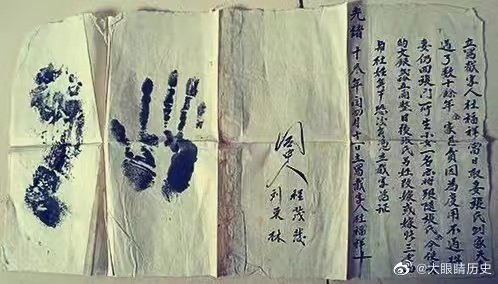
\includegraphics[height=0.36\textwidth,width=0.56\textwidth,viewport=0 0 375 240,clip]{Hand_and_foot-print.png}
\caption*{\hei 微博网页提供的清代光绪十八年~(公元1892年)~的休书}
\label{Collect_Liu_Wu}
\end{figure}
\includegraphics{.jpeg}

立写截字人杜福祥
当日娶妻张氏到家,夫妻过了数十余年。余家甚贫,因为度用不过,将妻仍回张门,所生小女一名,亦将跟随张氏。余今休妻的(得)文银贰拾伍两整,日后张氏另姓改嫁,或嫁张三、李四,与杜姓无干。恐说无凭,立截字为证。

\begin{flushright}
光绪十八年~闰四月十一日~立写截字人~~杜福祥 ~~(画 ``十字押'') ~~~\\

\large{同中人~程茂发、刘秉林} ~~~~~~~~~~~~~~~ \\

\huge{手模}、\huge{足印} ~~~~~~~~~~~
\end{flushright}

\newpage
\hypertarget{ux6253ux9c7cux6740ux5bb6-ux4e4b-ux8427ux6069}{%
\subsection{\texorpdfstring{打鱼杀家\protect\hyperlink{fn514}{\textsuperscript{514}}
之
萧恩}{打鱼杀家514 之 萧恩}}\label{ux6253ux9c7cux6740ux5bb6-ux4e4b-ux8427ux6069}}

\textbf{{[}第一场{]}}

\textbf{开船呐!}

\textbf{儿啊------}

\textbf{【西皮摇板】父女打鱼在河下,家贫哪怕人笑咱。拉住篷索父把网撒,}

\textbf{【西皮散板】年纪衰迈气力不佳。}

\textbf{唉,本当不做这河下生意,你我父女何以度日呀?}

\textbf{儿啊,不要啼哭,将船湾在柳荫之下,凉爽凉爽。}

\textbf{儿啊,将几尾鲜鱼烹煮好了,少时为父还要饮酒。}

\textbf{有人唤我。}

\textbf{是哪一位?}

\textbf{哦,原来是李贤弟。}

\textbf{敢莫要到舟中走走?}

\textbf{待我搭了扶手。}

\textbf{此位是------?}

\textbf{(惊介)这做什么?}

\textbf{老了,不中用了。}

\textbf{儿啊,出舱来见过二位叔父。}

\textbf{小女桂英。}

\textbf{一十六岁,痴长啊。}

\textbf{且慢,方才打得几尾鲜鱼,就在船头之上,你我弟兄畅快饮一回。}

\textbf{儿啊,看酒来。}

\textbf{啊,二位贤弟,愚兄有个酒令儿。}

愚兄做的是河下生意,忌的是``干''、``旱''二字。

不敢说罚,要敬酒三杯。

请------

呃,敬你三杯。

哦,待我看来。

诶!做什么的?

问的是哪一家呀?

你来看,就在前面,八字粉墙,合脊门楼,那就是丁\ldots{}\ldots{}

诶,哼,放肆!

量他也不敢呐。

请------

哦,又有人唤我。

二位贤弟再饮几杯。

哦,原来是丁郎儿,到此何事啊?

你来看,这几日天旱水浅,鱼不上网。改日有了银钱,送上府去。

哦,是是是。

放他去罢,

教他去罢。

(李俊、倪荣 啊,萧兄为何这等\ldots{}\ldots{}。)

他们的人多。

他们的势力大。

这就难讲话了。

本当不做河下生意,怎奈这囊中------唉,惭愧。

哪位贤弟送来?

当面谢过。

有了人家了。

花荣之子,名唤花逢春。

请------

二位贤弟慢走,愚兄不能远送了。

哦,来了。

儿问的是他?

儿啊------

\textbf{【西皮摇板】他本江湖二豪侠,倪荣、李俊就是他。蟒袍、玉带不愿挂,弟兄双双走天涯。}

\textbf{【西皮散板】猛抬头见红日坠落西斜。}

\textbf{儿啊,天色不早,我们回去了吧。}

\textbf{正是:(念)父女打鱼在江下,}

\textbf{(念)堪堪不觉红日落,}

{[}第二场{]}

\textbf{【西皮快三眼】昨夜晚吃酒醉和衣而卧,稼场鸡惊醒了梦里南柯。二贤弟在河下相劝与我,他教我把打鱼的事啊一旦丢却。我本当不打鱼啊关门闲坐,怎奈我家贫穷无计奈何。清早起开柴扉乌鸦叫过,飞过来叫过去【转西皮二六】却是为何。将身儿来至在草堂内坐,桂英儿取茶来为父解渴。}

\textbf{不教儿渔家打扮,怎么偏偏要渔家打扮?}

\textbf{呃------不听父言,就为不孝哇。}

\textbf{这便才是!}

\textbf{是哪个?}

\textbf{你们是哪里来的?}

\textbf{哦,原来是丁府上的教师爷。}

\textbf{哼!}

\textbf{做什么来了?}

\textbf{这几日天旱水浅,鱼不上网。改日有钱,送上府去,何必你来!}

\textbf{旁人来了无有,教师爷你来了么,}

\textbf{哼哼,越发的无有了!}

\textbf{朝廷王法,要它何用?}

\textbf{哼!}

\textbf{哼,尔要锁?}

\textbf{当真要锁?}

\textbf{果然要锁?}

\textbf{如此你就------锁!}

\textbf{不教锁。}

\textbf{哼!}

\textbf{话么,倒是两句好话呀,可惜呀可惜,}

\textbf{可惜你二大爷无有工夫啊。}

\textbf{尔要讲打?}

\textbf{诶呀!老汉幼年间,听说打架,如同小孩子穿新鞋、过新年的一般;如今呐------老了,打不动了啊!}

\textbf{尔当真要打?}

\textbf{果然要打?!}

\textbf{娃娃!待老汉将衣帽留在家中,打个样儿与你们见识见识。}

\textbf{【西皮导板】听一言不由我七窍冒火,}

\textbf{【西皮摇板】不由我年迈人咬碎牙车}\protect\hyperlink{fn515}{\textsuperscript{515}}\textbf{。江湖上叫萧恩不才是我,}

\textbf{【西皮摇板】大战场、小战场见过许多。爷本是出山虎独自一个,}

\textbf{【西皮摇板】尔好比看家犬一群一窝。你本是奴下奴敢来欺我。}

\textbf{慢说是三``羊头'',就是尔这三``狗头'',二大爷何惧!}

\textbf{你是丁府上的教师爷?}

\textbf{你好本领呐!老汉要领教领教。}

\textbf{一定要领教。}

\textbf{这是大十八般武艺?}

\textbf{这小十八样兵器?}

\textbf{这拳脚是?}

\textbf{软硬功夫?}

\textbf{呃,这叫什么?}

\textbf{不好哇。}

\textbf{这叫什么?}

\textbf{呃,不好。}

\textbf{呃,越发的不好啊。}

\textbf{方才撞了老汉三``羊头'',如今我要打你三拳头,放你过去。}

\textbf{哪里有功夫。}

\textbf{着打!}

\textbf{着打!}

\textbf{打得好,只恐打出祸来了!}

\textbf{那贼回去,定不甘休。待为父赶至县衙,抢他一个原告!}

\textbf{不要儿管,取为父的衣帽过来。}

\textbf{好好看守门户,为父去去就来。}\protect\hyperlink{fn516}{\textsuperscript{516}}

{[}第三场{]}

\textbf{(萧桂英
【西皮散板】老爹爹清晨出前去出首,)}\protect\hyperlink{fn517}{\textsuperscript{517}}

\textbf{(众 (内)一十!)}

\textbf{(萧桂英 【西皮散板】倒叫我桂英儿挂在心头。)}

\textbf{(众 (内)二十!)}

\textbf{(萧桂英 【西皮散板】将身儿来至在草堂门口,)}

\textbf{(众 (内)三十!)}

\textbf{(萧桂英 【西皮散板】只等得爹爹回细问根由。)}

\textbf{(众 (内)四十打完!)}

\textbf{(吕子秋 (内)赶下堂去!)}

\textbf{好贼!}

\textbf{【西皮散板】恼恨那吕子秋为官不正,仗势力欺压我受苦的良民呐。上堂来他那里一言不问,责打我四十板呐赶出了头门。}

\textbf{【西皮散板】我这里咬牙关忙往家奔,叫一声桂英儿你快来开门呐。}

\textbf{为父上得堂去,那贼一言不问,将为父重责。}

\textbf{这还不算受屈。他教为父连夜过江与那老贼赔礼,那才算受屈呢。}

\textbf{哎呀------我恨不得飞过江去,我就杀\ldots{}\ldots{}}

\textbf{我要杀贼的满门,方消我心头之恨!}

\textbf{小小年纪,懂得什么?!不用多管,取为父衣帽、戒刀过来。}

\textbf{不用儿管,快些取来。}

\textbf{为父去也。}

\textbf{何事?}

\textbf{小小年纪,去之无益。}

\textbf{有此胆量?}

\textbf{快将儿的衣服、兵刃收拾好了。}

\textbf{壮胆量也是好的。}

\textbf{走哇\ldots{}\ldots{}}

\textbf{做什么?}

\textbf{这门么,关也罢,不关也罢呀。}

\textbf{又做什么?}

\textbf{唉!门都不要了,还要什么家具呀?}

\textbf{唉,不明白的冤家呀,呃\ldots{}\ldots{}(哭介)}

\textbf{不要啼哭,随为父的走哇。}

\textbf{儿啊,此番前去,教儿骂,儿就骂,教儿杀,儿就杀,不要害怕。}

\textbf{走哇。}

\textbf{儿啊,夜晚行船,比不得白日,儿要掌稳了舵!}

\textbf{【西皮快板】这件事不由我心头冒火,今夜晚过江去将他杀却。恨不得插双翅江河越过,}

\textbf{【西皮散板】我的儿因何故放了篷索。}

\textbf{杀人还有什么假的不成?}

\textbf{呀呸!为父在家中不教儿前来,儿是偏偏地要来。这船行半江之中,儿又要回去------也罢!待为父拨转船头,送儿回去。}

\textbf{\textless{}哭头\textgreater{}啊,桂英,我的儿呀!}

\textbf{少时还在此处上船,儿记下了?}

\textbf{儿啊,庆顶珠}\protect\hyperlink{fn518}{\textsuperscript{518}}\textbf{可在身旁?}

\textbf{此番前去,倘有不测,儿自带庆顶珠逃往花家去吧。}

\textbf{我么------儿就不用管了哇。}

\textbf{不要啼哭,随我走哇。}

\textbf{来此已是。}

\textbf{且慢。}

\textbf{收拾好了。}

\textbf{有人么?走出一个来呀。}

\textbf{过府赔罪来了。}

\textbf{哼!}

\textbf{请了。}

\textbf{我来问你:这鱼税银子,可有圣上旨意?}

\textbf{户部公文?}

\textbf{凭着何来?}

\textbf{敢是那吕子秋?!}

\textbf{哼!}

\textbf{【西皮摇板】这税银我不纳是我的本分,你不该差人役打上我门。}

\textbf{儿啊,骂呀!}

\textbf{且慢,我父女有好心献上。}

\textbf{打鱼之时,得来一宗宝贝,名唤庆顶珠。}

\textbf{这\ldots{}\ldots{}耳目甚多。}

\textbf{看刀!}

\textbf{儿啊,随为父的杀呀!}

\newpage
\hypertarget{ux7843ux7802ux75e3-ux4e4b-ux97e9ux5ef7ux51e4ux8c2dux6d3e}{%
\subsection{硃砂痣 之
韩廷凤(谭派)}\label{ux7843ux7802ux75e3-ux4e4b-ux97e9ux5ef7ux51e4ux8c2dux6d3e}}

\textbf{{[}第一场{]}}

\textbf{唉!}

\textbf{【二黄摇板】为续弦前后厅灯光明亮,梦不想今夜晚再做新郎。}

\textbf{抬上堂来(或:}搭上堂来)\protect\hyperlink{fn519}{\textsuperscript{519}}\textbf{。}

\textbf{每人赏银二分(或:}每人赏钱四个)\textbf{。}

\textbf{带他们下面用饭。}

\textbf{待我观看一回。}

\textbf{【二黄慢板】我这里借灯光用目观望,我看她(或:只见她)与前妻一样风光。}

\textbf{【二黄慢板】为什么(或:因何故)皱眉间泪带面上(或:泪带脸上),莫不是嫌年迈难配鸾凰。}

\textbf{【二黄慢板】要穿衣锦绣衫任你选样,}

\textbf{【二黄慢板】要用饭现有那谷米陈仓。}

\textbf{【二黄慢板】这不是那不是难以猜想,尊娘行(或:问娘行)因何事珠泪汪汪,为的是哪桩,你何妨(或:又何妨)细说端详?}

\textbf{【二黄摇板】听她言这婚姻(或:好一似)冰结霜降,一时里惹动我烦恼愁肠。看起来断不可此事勾当,自情愿伴孤灯独守空房。}

\textbf{韩福过来。}

\textbf{命你同媒婆送这位大娘子回去,对他丈夫言讲(或:与他丈夫言讲):前番(那)一百两银子不要,再送他一百两银子,教他好好将养疾病,将大娘子送回,成全他夫妻恩义。就此去罢。}

\textbf{啊大娘子,还有这婚书呢。}

\textbf{唉,就在灯前焚化了罢。}

\textbf{【二黄摇板】伊言道她丈夫病卧床上,没奈何卖妻子暂度时光。将自己比旁人俱是(或:皆是)一样,我岂肯拆散他恩爱鸳鸯。(或:善与恶自有那天理昭彰。)}

\textbf{{[}第二场{]}}

\textbf{【二黄摇板}\protect\hyperlink{fn520}{\textsuperscript{520}}\textbf{】想当年为太守何等荣耀,遇兵荒妻和子无有下梢。多亏了陈太尉将我来保,才能得归田园自在逍遥。}

\textbf{【二黄摇板】忙迫中呃挽定了把礼还到,一时里好教我难解根苗。}

\textbf{呜,你不是昨晚送回去的大娘子么?}

\textbf{既然将你送回,你又来则甚呐?}

\textbf{哦,(原来是)吴相公来了。}

\textbf{哎呀,请坐请坐。}

\textbf{呃,还有话讲啊。}

\textbf{(有话叙谈,}哪有不坐之理,请坐请坐。\textbf{)}

\textbf{啊大娘子,你也坐下。}

\textbf{啊吴相公,昨日听得大娘子说到家中一番苦楚,甚是凄惨。相公有恙在身,改日再来叙谈,为何带病前来?(或:大相公,昨日听得大娘子说到家中一番苦楚。相公你有病在床,病体好了,再来不迟。)}

\textbf{哦,你见了银子,出了一身的通汗,这病就好了么?}

\textbf{哎呀呀,吴相公啊,看将起来,这银子啊,是好物件!}

\textbf{【二黄碰板垛板】我救你的急,救你的难,救你的贫困;全尔的节,全尔的义,全尔的婚呐姻。纵有妻不生子前生造定,我岂肯拆婚姻}\protect\hyperlink{fn521}{\textsuperscript{521}}\textbf{落下了骂名。}

\textbf{啊,啊,呵呵呵哈哈哈\ldots{}\ldots{}(笑介)}

\textbf{请坐请坐。}

\textbf{哎呀呀吴相公啊,我当日也是恩爱夫妻,只因兵荒马乱,中途失散,却无子嗣。若有一子传宗接代,我也就不续弦再娶的了哇。}

\textbf{这\ldots{}\ldots{}子孙前世所修,再续么,也就不必了。(或:}子孙之事,前生所修。再娶么,唉,也就不必了。\textbf{)}

\textbf{言得极是,只是本处孩儿多有不便呐。}

\textbf{本当如此,奈无机会。}

\textbf{这只好凭天机、遇时宜了。}

\textbf{吴相公慢些走啊!}

\textbf{【二黄摇板】他夫妻进门来双双拜倒(或:双双跪倒),口声声叫恩人泪似呃雨抛。非是我用银钱假意行好哇,韩廷凤全仁义一片心苗。}

\textbf{{[}第三场{]}}

\textbf{【四平调】叹光阴去不归无限烦闷,不觉已老两鬓如银。读古书难解我心头烦闷,饮香醪怎畅我衷肠凄清。}

\textbf{哦,你是吴相公,呃,请坐请坐。}

\textbf{你往成都收取账目,呃,必定是发了财了哇。(或:}闻你往成都,收取账目,一定发财的了。\textbf{)}

\textbf{请便。}

\textbf{哦,这是何人?}

\textbf{哦,罢了(罢了),一旁坐下。}

\textbf{呃,不妨不妨,只管地坐下。}

\textbf{呵呵呵哈哈哈\ldots{}\ldots{}(笑介)}

\textbf{啊吴相公,你看这小小的孩童,呃,也(很)知大体呀。}

\textbf{是啊,小孩子原要(他)爹娘教导哇。}

\textbf{啊吴相公,你买他前来,还是为子啊,还是为仆呢?}

\textbf{哦,这等说来(或:}如此说来)\textbf{,是送与我的?}

\textbf{哎呀呀吴相公啊,你真是(或:}你真乃)\textbf{信实人也。}

\textbf{【四平调】吴官人你真真言而有信,你与我谋后代不惜辛勤。感谢你这好意情深义尽,\textless{}行弦\textgreater{}}

\textbf{吴大哥,你请来上坐。(或:}这边坐,这边坐。\textbf{)}

\textbf{请坐,请坐。}

\textbf{【四平调】退一日自当另有条陈。}

\textbf{呵呵哈哈哈\ldots{}\ldots{}(笑介)}

\textbf{哎呀吴官人呐,我如今有了儿子就不愁了。}

\textbf{是啊,吴官人离家日久,我也不便相留(或:}不便强留\textbf{),改日我父子要登门叩谢。}

\textbf{儿啊,送过你吴大爷。}

\textbf{(啊,吴官人何事?)}

\textbf{请来吃酒,请来吃酒。}

\textbf{啊\ldots{}\ldots{}呃,吴官人,请转请转。}

\textbf{改日我父子,呃,要登门再谢。}

\textbf{呃一定要去,一定要去。}

\textbf{啊\ldots{}\ldots{}呃,无有了,请便请便。(或:}吴官人,请呐请呐。\textbf{)}

\textbf{哦------哈哈哈\ldots{}\ldots{}(笑介)}

\textbf{儿啊,随为父的进来。}

\textbf{一旁坐下,待我细看一回(或:待我}细观一回\textbf{)。}

\textbf{【二黄原板】我的儿须从容端然坐定,看形象并非是平等之人。细观他各部位五官端正,这两鬓齐开朗目秀眉清。儿在家可读过圣贤书本,一一地对为父细说分明。}

\textbf{【二黄原板】他说话有分寸智慧聪明,倒像个宦门后不差毫分。可记得是何年月日生辰,说出来将八字细与儿评。}

\textbf{【二黄原板】这小娃言语中隐藏暗景,再问他亲父母便知真情。儿父母年多少在不在,因何故图银钱卖与他人。}

\textbf{儿今年多大年纪了(或:}儿今年几岁了\textbf{) ?}

\textbf{儿父?}

\textbf{死了五载。}

\textbf{儿母?}

\textbf{七旬有余。}

\textbf{(惊介)儿有一十三岁(或:}儿才一十三岁\textbf{)。}

\textbf{(惊介)嗯\ldots{}\ldots{}}

\textbf{【二黄原板】这其间又盘出}\protect\hyperlink{fn522}{\textsuperscript{522}}\textbf{奇情种种,哪有个花甲年又产娇生。}

\textbf{儿啊------}

\textbf{【二黄原板】必然是那老娘将儿蒙混,这内中另有个生儿的娘亲。}

\textbf{哦,儿是捡来的么?}

\textbf{【二黄原板】细盘问这来由日月推论,仔细想当年事越加是真:宣和年四月里成都调任,行至在青州府路遇贼兵。亲生儿在娘怀无有踪影,实可怜贤德妻命赴幽冥。}

\textbf{【二黄散板】这形象好一似韩门真种,举动间与老夫骨肉有情。我这里取菱花照照相品呐,}

\textbf{【二黄散板】半像我半像妻不差毫分。}

\textbf{【二黄散板】亲生子再相逢三生有幸,这才是天地意弄假成真。}

\textbf{不对了,不对了!}

\textbf{(韩玉印 怎么不对呢?)}

\textbf{我那亲生的孩儿,落生下来,左足心上有硃砂红痣。你无有,不是我的亲生儿子啊。}

\textbf{怎么,儿也有?}

\textbf{为父的不信呐,待我看来。}

\textbf{(唉,儿啊------)}

\textbf{【二黄散板】你是我亲生的儿呀名唤玉印,遇兵荒遭失散十有二春。盼娇儿盼得我身染重病,盼娇儿盼得我昼夜不宁。盼娇儿啊不做官告归故呃井,喂呀我的儿呀,梦不想天保佑枯木哇逢春。}

\textbf{你母命丧东平,也曾命人搬尸去了\ldots{}\ldots{}哇,呃\ldots{}\ldots{}(哭介)}

\textbf{言得极是,派人接她前来就是。}

\textbf{正是:(念)北转南来西复东,今朝骨肉又重逢。父子再把菱花照,}

\textbf{(儿啊------)}

\textbf{(念)只怕相逢在梦中。}

\textbf{哦,不是做梦?}

\textbf{玉印,我儿,啊------啊------哈哈哈\ldots{}\ldots{}(笑介)}

\textbf{随我来。}

\newpage
\hypertarget{ux96c4ux5ddeux5173}{%
\subsection{雄州关}\label{ux96c4ux5ddeux5173}}

\textbf{{[}第一场{]}}

\textbf{呼延狄 (念)百万熊罴犯中原,}

\textbf{雷洪切 (念)搅乱宋室不安然!}

\textbf{达林呈 (念)渴饮马上刀头血,}

\textbf{季乐芬 (念)嘿!饥饿人头当饭餐!}

\textbf{众 俺------}

\textbf{呼延狄 金邦大将军呼延狄是也!}

\textbf{雷洪切 金邦副将军雷洪切是也!}

\textbf{达林呈 金邦左先锋达林呈是也!}

\textbf{季乐芬 金邦右先锋季乐芬是也!}

\textbf{萨里哈 前营骁骑大将军萨里哈是也!}

\textbf{耶律浑 后营骁骑大将军耶律浑是也!}

\textbf{提尔雄 左营压队大将军提尔雄是也!}

\textbf{虎骨达 右营护卫大将军虎骨达是也!}

\textbf{呼延狄 列位将军请了------}

\textbf{众 请了!}

\textbf{呼延狄
你我奉了狼主之命,随定四太子,领兵夺取宋室天下,兵到即克。也是宋王气数当尽了。}

\textbf{众 着啊!}

\textbf{呼延狄 这些蛮子怎能苦争恶战,这也是我家狼主洪福齐天也!}

\textbf{众
听觱篥}\protect\hyperlink{fn523}{\textsuperscript{523}}\textbf{一声响,太子升帐,你我两厢伺候。请------}

\textbf{金兀朮
\textless{}点绛唇\textgreater{}军营号响}\protect\hyperlink{fn524}{\textsuperscript{524}}\textbf{,威武雄壮;中军帐,排列刀枪,杀气呃------}

\textbf{众 参见殿下!}

\textbf{金兀朮 站立两厢!}

\textbf{金兀朮
(念)杀气腾腾满乾坤,哀声处处震天庭。宋王失政宠奸佞,锦绣江山一旦倾。}

\textbf{金兀朮
孤,北番大金邦女真国老王殿下四太子、昌平王、御营总兵完颜兀朮。今有宋主无道,宠信奸臣。内奸童贯封为广阳王}\protect\hyperlink{fn525}{\textsuperscript{525}}\textbf{之职。是他前者有密书到孤父王驾下,约定我国兴兵夺取他家社稷。有他以为内应,这宋室天下岂不是唾手而得。自兴兵以来,战无不胜,攻无不取。前日又破了潞安州,守将陆登自刎身亡,甚是悲惨。前面乃是雄州关,守将韩世忠。此人乃是忠勇之士,孤家不忍逼迫于他。意欲招他归顺,助孤一臂之力,何愁大事不成。}

\textbf{金兀朮 众番儿!}

\textbf{众 有!}

\textbf{金兀朮 此番兴兵行至雄州关,不可杀掠黎民,违令者斩!}

\textbf{众 啊!}

\textbf{金兀朮 由此发动人马!}

\textbf{{[}第二场{]}}

\textbf{探子 马来。}

\textbf{探子
(念)短甲随身衲袄齐,肩上横担令字旗。年年岁岁领皇赏。一马冲至军队里。}

\textbf{探子
俺,韩元帅麾下能行探子是也。奉了元帅将令,着俺四路哨探。今有圣上差孙浩督兵前来剿灭金邦,已至三山口。不免飞骑报韩元帅知道!就此马上加鞭。}

\textbf{{[}第三场{]}}

\textbf{韩世忠
【西皮三眼】为金兵急得我心神不定,盼救}兵望眼穿昼夜不宁。陆元帅尽了忠自刎丧命,只一子失陷在万马军营。好教人止不住啊【转\textbf{西皮二六}】腮边泪滚,可叹他夫妻们饮恨幽冥。行公文\protect\hyperlink{fn526}{\textsuperscript{526}}求圣上遣将助阵,因何故十数日渺无回音。在二堂思无计心呃中忧闷,我父子只恐怕难退雄兵。

中军 (念)探马如飞急,叩禀元帅知。

中军 启元帅:探马求见。

韩世忠 吩咐开门!

中军 开门!

众 啊!

韩世忠 \textbf{(念)}探马报音信,升帐问分明。

韩世忠 传探马。

中军 元帅有令:探马进见。

探马 报------告进。

探马 帅爷在上,探马叩头。

韩世忠 打听哪路军情,起来快些讲。

探马 啊,帅爷听禀:

探马
(念)一马哨探似流星,朝中差来孙总兵。十万人马到疆界,禀报元帅得知情。

韩世忠 朝中无有什么姓孙的呀!

探马 在元帅帐下当过副将的。

韩世忠 哦------敢是孙浩?!

探马 正是。

韩世忠 赏尔金牌一面,再去打探。

探马 得令!

韩世忠
且住!想那孙浩,在某帐下曾为副将。只因犯我将令,将他捆打,是他逃至京中,投在\textbf{广阳}府内,做了随侍。今番奉旨督兵前来,焉有不接之理。

韩世忠 中军!

中军 有!

韩世忠 传众将进帐。

中军 众将进帐呃!

\textbf{四将} (内)来也!

\textbf{四将}
(念)元帅传军令,将士共趋迎\protect\hyperlink{fn527}{\textsuperscript{527}}。

\textbf{四将} 参见元帅。

韩世忠 众位将军少礼!

\textbf{四将} 啊!

\textbf{四将} 传末将等进帐,有何军情议论?

韩世忠 圣上命孙浩督兵前来,征剿金人,已到三山口。命你等前去迎接。

\textbf{四将} 啊元帅,那孙浩若问:你家元帅为何不来。我等怎样回答?

韩世忠
你等就说:我家元帅因金兵犯境,城内空虚,不敢擅离汛地,故命我等前来迎接。

\textbf{四将} 那孙浩缘何授得此职?

韩世忠 唉!你等不知他的来历,听我令下:

\textbf{韩世忠
【西皮}原板】韩世忠坐宝帐传言发令,叫一声众将官细听详情:那孙浩平日间行为不正,犯军令责罚他不能徇情呃。逃到了京师地\textbf{广阳}府进,童太尉听谗言懵懂圣君。迎接他务须要言语谨慎,

\textbf{韩世忠 【西皮摇板}】防贼子寻仇起暗箭伤人。

\textbf{四将 得令!}

\textbf{四将 【西皮摇板】韩元帅忠义士谁人不敬,何惧那孙浩贼势利小人。}

\textbf{韩世忠
【西皮摇板】大宋朝八代君徽宗失政,贪酒色戮忠良信宠谗臣。恨蔡京与童贯伤害民命,惹得那四路里齐动刀兵。金兀朮领人马抢夺州郡,逼元戎劳将士苦及黎民。众将官退宝帐各归管汛,}

\textbf{韩世忠 【西皮摇板】且等候四将回再定计行。}

\textbf{{[}第四场{]}}

\textbf{孙浩
\textless{}点绛唇\textgreater{}奉旨领雄兵,蟒罗袍,不愧先人;定斩世忠消吾恨,还报他痛打军刑。}

\textbf{孙浩}
(念)\textbf{胸怀巧诈极聪明,不近贵人怎升腾?只道一生空劳力,运至时来命通亨。}

\textbf{孙浩
某,孙浩,塞北人也。昔在韩世忠麾下以为步军,只因不守军规,专意花酒情浓。抢得一有夫之妇作乐,不想韩世忠便要将俺斩首。是俺推在步兵列名身上,彼时将那步兵斩首号令。又道俺带领无方,将俺捆打,削去头领,赶出不用。俺又羞又恼,一怒奔至京中。恰遇童太尉朝罢而归,是俺闯了他的禁道,将我拿到府中拷问。俺将韩世忠打革之事从头诉说一遍,不想童太尉与韩世忠是旧有仇恨,听了此言,便把俺留在府呃中。因俺善于奉承,是他心中欢喜,想要重用于俺。如今金兀朮兴兵犯界,破了无数城池。眼看要到雄州,那韩世忠本章进京,求兵添将。童太尉奏上一本,命俺提兵前来,剿灭番贼。若是得胜,道韩世忠贪生怕死;若是损兵,便道韩世忠按兵不动。慢说是一个韩世忠,就是百个,也教他有死无生。看前面已是三山口,众将,催动人马!}

\textbf{孙浩 【西皮导板】见旌旗空中飘人声喧震,}

\textbf{孙浩
【西皮原板】抖起}了万丈尘沸沸腾腾。曾记得到京都那般光景,岂料我今日里督领雄兵。韩世忠好比那儿童之分,怎知晓暗中刀要你残生。咱料他如南柯梦魂未醒,

\textbf{孙浩 【西皮摇板}】绑云阳一命倾才晓前情。

\textbf{孙浩
前道}\protect\hyperlink{fn528}{\textsuperscript{528}}\textbf{为何不行?}

\textbf{四将 雄州关总戎麾下四营将校迎接总爷。}

\textbf{众 雄州关总戎麾下四营将校迎接总爷。}

\textbf{孙浩 传。}

\textbf{众 传。}

\textbf{四将 雄州关四营将校迎接总爷}

\textbf{孙浩 你家主帅有多大的官儿,怎么不来迎接本镇。}

\textbf{四将
启禀总爷:主帅为金兵临界,关内空虚,不敢擅离汛地,故而命末将等前来迎接总爷。}

\textbf{孙浩
哼------你住了!本镇钦奉圣命,广阳王钧旨,领兵剿贼,你们主帅也不看在眼内,本当将尔等捆打------}

\textbf{四将 总爷开恩。}

\textbf{孙浩 也罢!待本镇破了金兵回来,再与你主帅辩理。}

\textbf{孙浩 来呀,乱棍逐出!}

\textbf{孙浩 催------军!}

\textbf{孙浩
【西皮摇板】定教他主帅们无处逃奔,少不得斩尔等碎尸粉身。叫众将越过了飞龙奇岭,扫灭了番邦贼奏达捷音。}

\textbf{{[}第五场{]}}

\textbf{韩世忠
【西皮摇板】命四将接孙浩渺无音信,倒教我背地里暗自思忖呐。必然他要报那从先的仇恨,可惜我空费了一片精神。}

\textbf{四将 【西皮摇板】贼孙浩忒无礼令人可恨,全不念数年间共事同营。}

\textbf{四将 参见元帅!}

\textbf{韩世忠 你们回来了。}

\textbf{四将 回来了。}

\textbf{韩世忠 迎接孙浩他可曾讲些什么?}

\textbf{四将 末将等奉令迎接孙浩,那厮言道:你家主帅为何不来?}

\textbf{韩世忠 你等怎生回答?}

\textbf{四将
末将言道:金兵临界,城内空虚,不敢擅离汛地,故命我等前来迎接}

\textbf{韩世忠 那厮如何言道?}

\textbf{四将
那厮言道:本镇钦奉圣命,广阳王钧旨,领兵剿贼,你主帅有多大的官儿,不来迎接本镇。本当将尔捆绑------待等破了金兵回来,再与你主帅辩理。说罢此言,呃,将我等乱棍,呵,逐出来了。}

\textbf{韩世忠 小人得志,以致如此。}

\textbf{探子 报!启禀元帅:孙浩越过飞龙岭,迎战金兵去了。}

\textbf{韩世忠 再探!}

\textbf{韩世忠
且住!我想孙浩越过飞龙岭与金兵迎战,倘有差池本帅难逃罪责。}

\textbf{韩世忠 来,传彦直进帐。}

\textbf{中军 有请少将军。}

\textbf{韩彦直 来也!}

\textbf{韩彦直 (念)战国英雄数伍员,一忿扫平楚国兵。}

\textbf{韩彦直 参见父帅。}

\textbf{韩世忠 罢了!坐下。}

\textbf{韩彦直 谢座。唤孩儿进帐,有何吩咐?}

\textbf{韩世忠
圣上命孙浩督兵前来,征剿金人,那贼从飞龙岭迎敌去了。命你带领人马,暗地保护,需要小心在意,听为父令下:}

\textbf{韩世忠
【西皮摇板】广阳王点孙浩身当重任,命四将迎接他赶回州城。我的儿领人马暗地接应,钦命官须保护谨慎小心。}

\textbf{韩彦直 得令!}

\textbf{韩彦直
【西皮摇板】在帐中领将令怎敢迟顿,暗地里保孙浩谨慎殷勤。}\protect\hyperlink{fn529}{\textsuperscript{529}}

\textbf{韩世忠 众将官,随本帅披挂,催动人马,起兵前往!}

\textbf{{[}第六场{]}}

\textbf{金兀朮 马前来的将官,可是韩元帅?}

\textbf{孙浩 逆贼,俺乃童太尉府中的心腹之人,剿贼大将军孙浩是也!}

\textbf{金兀朮 奸贼一党,休要放走之呃!}

\textbf{{[}第七场{]}}

\textbf{韩彦直
(念)头戴束发紫金冠,金锁铠甲扣连环。胸怀重瞳英雄胆,宝剑出鞘血未干。}

\textbf{韩彦直 俺,韩彦直。奉了父帅之命,暗地保护孙浩。}

\textbf{韩彦直 众将官!}

\textbf{众 有!}

\textbf{韩彦直 杀上前去!}

\textbf{{[}第八场{]}}

\textbf{探子 启元帅:孙浩落马;少爷杀进番营去了!}

\textbf{韩世忠 再探!}

\textbf{韩世忠 且住!孙浩落马,我儿杀进番营,这还了得!}

\textbf{韩世忠 众将官,}

\textbf{众 有!}

\textbf{韩世忠 奋勇当先!}

\textbf{{[}第九场{]}}

\textbf{金兀朮
住了,你这小儿,二次杀进番营,倒有些胆量,饶尔不死,通名上来!}

\textbf{韩彦直 听者:俺乃雄州关总戎之子韩彦直是也。}

\textbf{金兀朮 你就是韩世忠之子么?!}

\textbf{韩彦直 然也。}

\textbf{金兀朮 哎,真乃是将门之子!}

\textbf{韩彦直 呔,番贼通名受死。}

\textbf{金兀朮 孤乃大金邦四太子昌平王兀朮是也。}

\textbf{韩彦直 着打!}

\textbf{韩世忠 彦直,孙浩何在?}

\textbf{韩彦直 被番兵踹为肉泥。}

\textbf{韩世忠 好哇!儿啊,下马来,为父有话言讲。}

\textbf{韩彦直 是。}

\textbf{韩世忠 好奴才!}

\textbf{韩世忠
【西皮散板】为父怎样将儿命,断送孙浩丧番营。金枪刺儿咽喉哽,}

\textbf{韩彦直 【西皮散板】要杀孩儿为何情?}

\textbf{韩世忠
大胆畜生,为父可曾}\protect\hyperlink{fn530}{\textsuperscript{530}}\textbf{吩咐与你?!那孙浩乃是圣上差来,又是广阳王的保举,教儿小心暗护,竟被番营杀死,倘若圣上闻知,必道为父有按兵不动之罪。哎呀!儿啊!岂不把为父的送在枉死城去?!}

\textbf{韩彦直
哎呀,爹爹呀!孩儿奉命暗护孙浩,杀进番营,并无此人。况且儿又不认识于他。}

\textbf{韩世忠 住了!那孙浩乃是领兵元戎,必有旗号,儿也不认得吗?}

\textbf{韩彦直
哎呀,爹爹呀!孩儿虽然奉令暗护孙浩,但是万马营中,犹如刀山剑岭,难道教儿束手待死不成?!}

\textbf{四将 元帅,公子之言甚是,还望元帅开恩。}

\textbf{韩世忠
也罢,命儿三次杀进番营,杀退番邦便罢,如若不然,定斩尔的首级。}

\textbf{韩彦直 得令呐!呵\ldots{}\ldots{}(哭介)}

\textbf{韩世忠 哼!}

\textbf{韩世忠 众将官,直踹番营!}

\textbf{{[}第十场{]}}

\textbf{金兀朮 呔,马前来的敢是韩元帅?}

\textbf{韩世忠 然。马前搭话敢是兀朮?}

\textbf{金兀朮 然。}

\textbf{韩世忠
兀朮!吾主有何亏负尔等,既破潞安州,又来兵犯吾郡,是何理也?}

\textbf{金兀朮
韩元帅,你且停战马,听某一言告禀:你主贪淫失政,宠信奸佞,忠良遭戮,以致刀兵四起。莫若归顺我邦,得了宋室天下,定是三台鼎鼐之位。元帅上察!}

\textbf{韩世忠
兀朮,你韩元帅兵虽少个个勇。你强夺州郡}\protect\hyperlink{fn531}{\textsuperscript{531}}\textbf{,伤害人民,恨不得食尔之肉,还敢多言么?}

\textbf{韩世忠
【西皮摇板】战鼓嗵嗵山岳动}\protect\hyperlink{fn532}{\textsuperscript{532}}\textbf{,番邦贼寇敢逞能。扫灭狼烟归大宋,方显男儿是英雄。}

\textbf{金兀朮 韩元帅。}

\textbf{金兀朮
【西皮摇板】久闻世忠武艺灵}\protect\hyperlink{fn533}{\textsuperscript{533}}\textbf{,今日见面果俊英。堂堂仪表非俗品,胜似战国楚伍员。}

\textbf{金兀朮 韩元帅。}

\textbf{金兀朮 【西皮摇板】你若马前来归顺,孤家与你皇兄称。}

\textbf{韩世忠 住了!}

\textbf{韩世忠
【西皮摇板】兀朮开言真堪恨,气得本帅怒上升。收兵回马保众命,不然杀尔草寇平。}

\textbf{{[}第十一场{]}}

\textbf{韩世忠 参见圣上!}

\textbf{童贯
韩世忠!按兵不动,陷害朝廷命官,有降顺金邦之意!来啊!打入囚车!}

\textbf{韩世忠 唉呀!}

\textbf{探子 报!金兵四面围困。}

\textbf{童贯 再探!}

\textbf{童贯 唉呀!}

\textbf{童贯 也罢!韩世忠,命你杀退金兵,将功折罪呀!}

\textbf{韩世忠 奋勇当先!}

\textbf{金兀朮 好小子呃!}

\textbf{韩世忠 追呃!}

\textbf{韩世忠 哈哈,哈哈,啊------呵呵哈哈哈\ldots{}\ldots{}(笑介)}

\textbf{韩世忠 收兵呐!}

\newpage
\hypertarget{ux9547ux6f6dux5dde-ux4e4b-ux5cb3ux98deux6768ux749f}{%
\subsection{镇潭州 之
岳飞、杨璟}\label{ux9547ux6f6dux5dde-ux4e4b-ux5cb3ux98deux6768ux749f}}

\textbf{{[}第一场{]}}

\textbf{岳飞
\textless{}点绛唇\textgreater{}报国精忠,虎啸龙吟;迎二圣,扫荡烟尘,保主锦绣春。}

\textbf{岳飞
(念)旌旗招展出禁城,武将心思汗马勋。剖心要尽凌云志,迎回二圣方称心。}

\textbf{岳飞
本帅,姓岳名飞字鹏举,宋室驾前为臣。只因奸佞当道,张邦昌陷二圣于沙漠,坐井观天。是我退归林下;今蒙太后二次诏宣,官拜天下都招讨、兵马大元帅;后宫娘娘恩赐五色锦旗,亲绣``精忠报国''。}

\textbf{岳飞
本帅亲承王命,统领六师,扫荡烟尘,恢复河山。今乃黄道吉日,正好兴兵。众位贤弟!}

\textbf{岳飞 人马可齐?}

\textbf{岳飞 香案伺候!}

\textbf{岳飞
祝告:(念)山川社稷、万里旗纛尊神:信官岳飞,今奉圣命,扫荡九龙山杨再兴、长沙王罗延庆、洞庭湖水贼杨幺等。但愿此行,旗开得胜!}\protect\hyperlink{fn534}{\textsuperscript{534}}

\textbf{岳飞 打道出府。}\protect\hyperlink{fn535}{\textsuperscript{535}}

\textbf{岳飞 牛皋听令。}

\textbf{岳飞 命你去到潭州晓谕节度使,命他高垒城郭,本帅大兵随后就到。}

\textbf{岳飞 转来。}

\textbf{岳飞 岳云听令。}

\textbf{岳飞 解押粮草}

\textbf{岳飞 张宪听令。}

\textbf{岳飞 催运粮草}

\textbf{岳飞} 张保\textbf{听令。}

\textbf{岳飞 命你以为总督粮官。}

\textbf{岳飞 吉青听令。}

\textbf{岳飞 随营护卫。}

\textbf{岳飞 施全听令。}

\textbf{岳飞
命你总督三军。}传令下去,众将一路之上,不可马踏青苗,扰害百姓,违令者斩!

\textbf{岳飞} 就此起兵潭州。

\textbf{{[}第二场{]}}

\textbf{岳飞 哦,恩师!}

\textbf{岳飞 不敢,恩师请!}

\textbf{岳飞 门生放肆。}

\textbf{岳飞 门生有何德能,敢劳恩师迎接十里之外?}

\textbf{岳飞 惶恐啊惶恐!}

\textbf{岳飞 我命牛皋前来,为何不见?}

\textbf{岳飞 哦,牛皋至此,未憩鞍马,径自立功去了?}

\textbf{岳飞 嗯------想他此去,必然是大败而归。}

\textbf{岳飞 贤弟,你与敌人交战,胜负如何?}

\textbf{岳飞 怎么样?}

\textbf{岳飞 可曾问过敌人的名姓?}

\textbf{岳飞
呃------你跟随愚兄出兵多年,还是这样粗鲁,倘若得胜而归,教愚兄怎上功劳簿。}

\textbf{岳飞 敢是那杨再兴?}

\textbf{岳飞 此人英勇无敌,你岂是他人对手,待本帅亲自会他。}

\textbf{岳飞
众位贤弟!有所不知,想那杨再兴,乃是将门之子,名门之后,武艺高强,本帅意欲,将他收留帐下,做一膀臂。今日出马,非比寻常,众将只许观阵,不许助战,违令者斩!}

\textbf{岳飞 恩师不必拦阻,待门生先见一阵。}

\textbf{岳飞 就烦恩师谨守城池。}

\textbf{岳飞 众将官,带马迎敌者。}

\textbf{岳飞 杨将军,别来无恙!}

\textbf{岳飞 杨将军,想那年在汴梁小校场,会过一面,难道将军你就忘怀了?}

\textbf{岳飞 然也。}

\textbf{岳飞
杨将军,想你乃是将门之子,忠良之后,因甚事失身落草,岂不玷辱杨氏祖先?听本帅相劝,归顺皇朝,共灭金寇,不失封侯之位,将军三思。}

\textbf{岳飞 住口!好言相劝,执意不听,少时擒在马前,悔之晚矣!}

\textbf{岳飞 决一胜负。}

\textbf{岳飞 这个\ldots{}\ldots{}杨将军,俺若不胜,情愿将潭州奉让。}

\textbf{岳飞
杨将军,你我今日交战,非比寻常,必须一对一个;两下各传将令,众将只许观阵,不许助战,违令者斩。}

\textbf{岳飞 军令不严非为丈夫也。}

\textbf{岳飞 \textless{}叫头\textgreater{}众将官!}

\textbf{岳飞 只许观阵,不许助战,违令者斩!}

\textbf{岳飞 【西皮小导板】叫三军与爷战鼓操,}

\textbf{岳飞
【西皮快板】马前闪出一英豪。杨家世代把国保,因何埋名在山巢。劝你马前归顺好,封妻荫子永在朝。}

(上手(岳飞)大边,一扯两扯,幺二三往外把盖下手(杨再兴)枪左转身(下手右转身)到里边打一个腰封、两个腰封,被往里面盖右转身(下手左转身)到外边,接一个腰封、两个腰封,把盖撤枪,撤右脚斜向上场门,上左脚刺在上场边里面的下手左右两马腿,左刺耳\protect\hyperlink{fn536}{\textsuperscript{536}},被下手盖,撤枪撤左腿在下场门边外面接下手两个刺马腿,盖下手左刺耳,搭、拉归里边面外、下手面里,搭、兜转身过到小边,面对过大边的下手掣肘,撤枪两人对脸左右左三个刺马腿,一二三绕、边绕边走从外面过到大边,一二三绕,边绕边走从外面过到小边,下手向内侧刺上手马腿、上手挑起向里刺肚,从里边左转身到外边向外侧刺下手马腿、下手挑起来刺肚,下手直着过到小边,上手接刺肚向右反转身从里边过到大边,二人合身往里一盖两盖,上手手平伸扎下手一枪左转身(下手左手拿枪滑上手扎出的枪、右转身右手掏翎,送到嘴叼翎,枪交右手),上手左手捋胡子、跨右腿、左转身又扎下手一枪(下手右手枪滑上手枪,右转身左手掏翎子),上手转过来扔胡子、枪收回来平托、左手山膀,大边里边站斜向外亮住(下手转过来右手枪剜萝卜、右手伸出、枪头斜向下,左手拿翎横胸前,弓箭步外边站斜向里亮住)\protect\hyperlink{fn537}{\textsuperscript{537}}

(拉上、斜亮,到台口正亮,一二三夺换位亮,一二三夺分开,一合两合,岳飞归小边,幺二三岳被勾走马腰封到大边、再被一压、被漫头左转身到中间面向里一别(杨同时归中间里面向外一别),岳飞撤枪向里面斜刺、刺空(杨出枪贴岳背扎脖),岳飞左转身用枪杆把杨枪搕出去、捋胡子下,杨望岳捋枪向外望、斜托枪亮住,耍下场追下)\protect\hyperlink{fn538}{\textsuperscript{538}}

\textbf{岳飞 绑了!}

\textbf{{[}第三场{]}}

\textbf{岳飞 杨将军,你我再决胜负。}

\textbf{岳飞 回营!}

\textbf{{[}第四场{]}}

\textbf{岳飞 将岳云绑了上来!}

\textbf{岳飞 小奴才,何人教你出马?何人教你出马?}

\textbf{岳飞
大胆奴才!想那杨再兴,乃是将门之后,为父指望收服于他,作为膀臂。故而不许旁人助战,你众位叔父都不敢违抗为父的将令,惟有你这小畜生,你敢犯我的军规吗?}

\textbf{岳飞 斩!}

\textbf{岳飞 众位贤弟,敢是与奴才讲情?}

\textbf{岳飞 可知本帅令出山岳动,这言发------神鬼惊!}

\textbf{岳飞 斩!}

\textbf{岳飞 \textless{}叫头\textgreater{}岳云,奴才!}

\textbf{岳飞 怎么你要回去见你那祖母、娘亲么?}

\textbf{岳飞 掌起面来!}

\textbf{岳飞 \textless{}三叫头\textgreater{}岳云,娇儿,唉,儿啊!}

\textbf{岳飞 为父今日要将儿斩首,怎么你要回去见你那祖母、娘亲么?}

\textbf{岳飞 嗯,只怕儿今生今世就不能相见了。}

\textbf{岳飞 斩!}

\textbf{岳飞 赦了。}

\textbf{岳飞 将岳云带了上来!}

\textbf{岳飞
奴才,本当将你斩首,念在你众位叔父苦苦讲情,死罪已免,活罪难容。}

\textbf{岳飞 牢子手,将奴才重责四十!}

\textbf{岳飞} 张保\textbf{听令!}

\textbf{岳飞
命你押解岳云,去到杨再兴营盘,对他言讲:岳云解粮在先,本帅传令在后,不知有此军令,在阵前冒犯将军,回营就要斩首;多亏满营将官讲情,死罪已免,活罪难容,重责四十,请将军验伤。上覆杨将军,明日还在阵前相会。掩门!}

\textbf{{[}第五场{]}}

\textbf{杨璟 (念)生前为大将,死后做忠魂。}

\textbf{杨璟
吾乃杨璟阴魂是也。今有孙男再兴,落草为寇。岳元帅难以收服,我不免去至宋营,梦中授他撒手金锏,助他成功。}

\textbf{杨璟 鬼卒,宋营去者。}

\textbf{杨璟
【二黄原板】我杨家祖居在梅花山后,老王爷锤换带才把宋投。都只为再兴儿落草为寇,岳元帅无良谋难把他收。教鬼卒前引路宋营来走,见了那岳元帅细}说从头。

\textbf{{[}第六场{]}}

\textbf{岳飞
【二黄原板】清晨起打一仗龙争虎斗,战不过杨再兴脸面惭羞。在虎帐传一令严加防守,迎二圣我才得展放眉头。}

\textbf{杨璟 【二黄摇板】听谯楼打罢了三更时候,到宋营见元帅细说根由。}

\textbf{岳飞 请问老先生尊姓大名,家住哪里,来到我营有何贵干?}

\textbf{杨璟 老夫祖居磁州梅花山后,杨璟是也。}

\textbf{岳飞 哦,原来是前辈老先生,失敬了。老先生有何见谕?}

\textbf{岳飞 元帅受我一礼。}

\textbf{岳飞 老先生施礼为何?}

\textbf{杨璟 只因孙儿再兴,不幸失身落草,还望元帅加以收服。}

\textbf{岳飞 本帅倒有此意,怎奈再兴武艺高强,难以收服。}

\textbf{杨璟 杨家梅花枪暗藏撒手锏,待老夫传授与你。}

\textbf{岳飞 领教了!}

\textbf{杨璟 【二黄摇板】我杨家梅花枪暗藏撒手,}

\textbf{岳飞 【二黄摇板】老先生秉忠心万古名留。}

\textbf{杨璟 【二黄摇板】但愿得收服他鞍前马后,}

\textbf{岳飞 【二黄摇板】他本是将门子啊必定封侯。}

\textbf{杨璟 【二黄摇板】哗喇喇打开了玲珑甲胄,}

\textbf{(众 \ldots{}\ldots{}醒来。)}

\textbf{岳飞 【二黄散板】多蒙你进帐来枪锏传授。猛然间又只见红日当头。}

\textbf{(报子 再兴讨战。)}

\textbf{岳飞 带马阵前去者。}

\textbf{岳飞 杨将军,昨日小儿阵前多有冒犯!}

\textbf{岳飞 岂敢。你我今日再决胜负。}

\textbf{岳飞 话出不悔,真丈夫也。放马过来。}

\textbf{(岳飞、杨再兴开打)}

\textbf{岳飞 杨将军,本帅失手了。}

\textbf{岳飞 弃暗投明,真乃俊杰也。欲与将军结为金兰,万勿见却?}

\textbf{岳飞 不必推辞,你我望空一拜。}

\textbf{岳飞 不必查点,兵合一处。}

\textbf{岳飞 众将官,同进潭州!}

\newpage
\hypertarget{ux516bux5927ux9524}{%
\subsection{八大锤}\label{ux516bux5927ux9524}}

\textbf{{[}第一场{]}}

\textbf{(【撤锣】【帽子头】王佐上)}

\textbf{王佐 (念)若为(或:欲为)天下奇男子,须立人间未有功。}

\textbf{探子 陆文龙讨战。}

\textbf{岳飞 再探!}

\textbf{探子 得令!}

\textbf{岳飞
\textless{}叫头\textgreater{}天呐,天!番邦出了陆文龙,此乃------天亡宋也。}

\textbf{王佐 啊元帅,想那陆文龙,敢莫是当年潞安州节度使陆登之子么?}

\textbf{岳飞 正是。}

\textbf{王佐 闻得他父命丧金人之手,如今为何反助仇人?}

\textbf{岳飞
贤弟哪里知道,当初金兵大破潞安州,此子未满三月,他怎能知晓。}

\textbf{王佐
也罢,待俺王佐,诈降番营。顺说陆文龙来降,不知元帅意下如何?}

岳飞 唉,贤弟,画虎不成反类其犬。哎,你料理军务去吧。

\textbf{王佐 是,告呃退。}

\textbf{岳飞 众将官,小心防守。}

{[}第二场{]}

\textbf{(王佐 唉!)}

\textbf{王佐 【二黄导板】听谯楼打初更玉兔东上,}

\textbf{王佐 【回龙】为国家、秉忠心、食君禄、报王恩,昼夜奔忙。}

\textbf{王佐
【二黄原板】想当年在洞呃庭逍遥放荡,到如今食君禄未报宋王。岳大哥他待我手足一样,我王佐无功劳怎受荣光?今夜晚思一计番营去闯,落一个美名儿万载传扬。}

\textbf{王佐
想}俺(或:想我)王佐,自投宋以来,寸功未立。今日岳元帅杀得大败。俺王佐
若能思得一计,诈降番营,顺说陆文龙来降,岂不是大功一场,名垂千古?

\textbf{王佐
【二黄原板】怎能够今夜晚番营得进,前后话向文龙细说真情(或:衷情)。}

\textbf{王佐 【二黄原板】前也思、后又想无有计定,倒不如上公案细看古今。}

\textbf{王佐 《前唐》?}

\textbf{王佐 不好哇!}

\textbf{王佐 《后汉》!}

\textbf{王佐
呜哙呀!想汉室卫律、苏武,同往北国催贡,一个降顺番邦,一个打入羊群,食
毡饮雪,还是忠心不改,与岳大哥一般无二矣!}

\textbf{王佐
【二黄原板】汉室中(或:汉朝中)卫律声名不正,却为何那苏武一片丹心。饥食毡、渴饮雪忠心耿耿,天保护、地保佑暗有神灵。}

\textbf{王佐 《后汉》?}

\textbf{王佐 不好呃!}

\textbf{王佐 《(东周)列国(志)》。}

\textbf{王佐 还是看看《列国》罢。}

\textbf{王佐 ``要离断臂刺庆忌'',``要离断臂刺庆忌''\ldots{}\ldots{}}

\textbf{王佐
且住,想那要离断臂,刺死公子庆忌,(此)乃大丈夫所为,俺王佐何不学他一学?}

\textbf{王佐
【二黄散板】那要离呀断臂行果有志量(或:颇有志量)呐,留下了美名儿万载传扬。我王佐学断臂番营呐去闯啊,顾不得生和死啊天作主张。}

\textbf{旗牌 (王将军)醒来!)}

\textbf{王佐
【二黄散板】霎时间痛得我神魂不定,好一似滚油煎乱箭攒心。睁开了昏花眼难以扎挣,为国家斩断臂要留美名。}

\textbf{旗牌 将军为何如此?}

\textbf{王佐
尔等不可声张。来来来,这有书信一封,送往大帐(或:送到大帐)岳元帅。就说我,呃,另有公干去了哇。}

\textbf{旗牌 遵命。}

\textbf{王佐 转来。}

\textbf{旗牌 在。}

\textbf{王佐 千万不可走漏风声。}

\textbf{旗牌 遵命。}

\textbf{王佐 且住,趁此天色朦胧,我不免诈降番营去者。}

\textbf{王佐 呼------呜\ldots{}\ldots{}}

{[}第三场{]}

\textbf{旗牌 有请元帅。}

\textbf{岳飞 (念)闷坐大营无良计,愁思昼夜费心机。}

\textbf{岳飞 何事。}

\textbf{旗牌 王将军书信呈上。}

\textbf{岳飞 待我看来。}

\textbf{岳飞 呜哙呀,原来王贤弟诈降番营去了。}

\textbf{岳飞 来,王贵进帐。}

\textbf{王贵 参见元帅。}

\textbf{岳飞 命你巡营瞭哨,待等王佐将军消息。需要小心!}

\textbf{王贵 得令!}

{[}第四场{]}

\textbf{金兀朮 (念)兴兵攻宋室,}

\textbf{陆文龙 (念)一战建奇功。}

\textbf{金兵 启狼主,拿住奸细一名。}

\textbf{金兀朮 押进帐来。}

\textbf{王佐 叩见狼主。}

\textbf{金兀朮 唗!大胆奸细,竟敢前来窥探。来------推出斩了!}

\textbf{王佐 (啊)慢来慢来,留头讲话呀。}

\textbf{陆文龙 啊,是啊,父王要留头讲话。}

\textbf{金兀朮 你且讲来。}

\textbf{王佐
是。难臣王佐,乃岳飞帐下一名随营参军。见他屡次杀得大败,是我劝他归降(或:
归顺);(不想)他是执意不肯。当时拔剑,断臣左臂,言道:誓要扫灭金邦,迎
请二圣还朝,然后再将难臣斩首。哎呀狼主啊!如今,我死又死不了,活是活受
罪呀!唉,狼主救命呐,呃\ldots{}\ldots{}(哭介)}

\textbf{金兀朮 孤家不信,一派谎言。}

\textbf{王佐 现有断臂(在此)为证。}

\textbf{金兀朮 我却不信。}

\textbf{王佐 狼主请看------}

\textbf{金兀朮 呜哙呀,岳飞呀岳飞,降与不降,但凭于你。为何下此毒手?!}

\textbf{金兀朮 罢了,你起来,孤家收留于你也就是了。}

\textbf{王佐 谢狼主!}

\textbf{金兀朮 如今归顺我国,就是我国人了,必须与你改个名字。你叫什么?}

\textbf{陆文龙 是呀,要改个名字的才是。他叫什么?}

\textbf{王佐 唉,苦------哇!呃\ldots{}\ldots{}(哭介)}

\textbf{金兀朮 有了有了,你为孤家吃了苦了。就叫作``苦人儿''罢!}

\textbf{陆文龙 ``苦人儿''------呵,甚好。}

\textbf{王佐 是。}

\textbf{金兀朮 我命太医与你调治伤痕。满营之中,任你闲游。出帐调治去罢。}

\textbf{王佐 是,谢狼主。}

\textbf{王佐 呼------呜\ldots{}\ldots{}}

\textbf{金兀朮 啊,儿啊,}为父已命人去搬取铁浮图,攻打宋营。正是:

\textbf{金兀朮 (念)}恼恨岳飞太不仁,

陆文龙 \textbf{(念)}军中哪有断臂刑!

{[}第五场{]}

\textbf{(乳娘
【二黄摇板】何日里才能得冤冤相报,思想起当年事心似火烧。撇故土到他乡谁为倚靠,屡次里想回国无路可逃。}\protect\hyperlink{fn539}{\textsuperscript{539}}\textbf{)}

\textbf{王佐 走哇!}

\textbf{王佐
【二黄摇板】这几天到番营未有巧机}\protect\hyperlink{fn540}{\textsuperscript{540}}\textbf{,怎能够向他人来把话提(或:细说端的;细说端倪)。}

\textbf{王佐 来此已是陆文龙的营盘,待我来偷觑偷觑。}

\textbf{乳娘 啊------哪里来的奸细,小番,与我拿下了。}

\textbf{王佐
啊老太太,莫要高声呐。(我不是奸细呀,)我就是狼主新收下的一个残废人,
取名``苦人儿'',就是我哇。}

\textbf{乳娘
啊,不错不错。殿下言道,有一南朝将官,名唤王佐,投顺我邦,改名``苦人
儿'',呃,就是足下么?}

\textbf{王佐 正是!}

\textbf{乳娘 哦,我们是幸会呀。}

\textbf{王佐 幸会呀。}

\textbf{王佐 啊老太太,听你讲话,不像此地(或:此处)人氏啊。}

\textbf{乳娘 本不是此地人氏。}

\textbf{王佐 哪里人氏?}

\textbf{乳娘 老身乃是湖广潭州人氏。}

\textbf{王佐 哦,老太太,你是湖广潭州人么?}

\textbf{乳娘 正是。}

\textbf{王佐 呵呵,这倒巧得紧(或:这倒巧得很)呐,我也是湖广潭州人呐。}

\textbf{乳娘 哦,如此说来,我们是同乡?!}

\textbf{王佐 是同乡啊。}

\textbf{(乳娘 重见一礼。)}

\textbf{王佐 好,重见一礼。}

\textbf{乳娘 (念)久旱逢甘雨,}

\textbf{王佐 (念)他乡遇故知。}

\textbf{王佐 啊,老太太你缘何至此?}

\textbf{乳娘
噤声!我与将军乃是同乡,说也无妨:老身薛氏,当年在潞安州陆登陆大老爷府
中,以为乳娘;那年金兵打破城池,老爷、夫人尽忠、尽节而死,撇下未满三
月的陆公子,,被狼主捉回金邦,算来一十六载。唉,陆家的冤仇何日得报哇,
啊,啊\ldots{}\ldots{}(哭介)}

\textbf{(王佐 哦哦哦,是是是\ldots{}\ldots{})}

\textbf{王佐 唉!实实地可怜呐!}

\textbf{乳娘 唉!实实地可怜呐!}

\textbf{王佐 啊老太太,(但不知)那陆公还有后么?}

\textbf{乳娘
怎说无有呃,昨日在两军阵前,连挑宋将数员上将}\protect\hyperlink{fn541}{\textsuperscript{541}}\textbf{,那不就是陆公子么。}

\textbf{王佐 哦?那就是陆公子么?}

\textbf{乳娘 嗯,正是。}

\textbf{王佐 呵呵,我王佐今日来的好机会也!}

\textbf{王佐
【二黄摇板】听罢言来喜心上,尊声安人听端详:我断臂原本为小殿下呀,舍死忘生到番邦。}

\textbf{乳娘 如此说来,呃,你为我家公子吃了苦了哇!}

\textbf{王佐 呜------不妨啊。}

\textbf{王佐
【二黄摇板】这断臂的情由休声嚷啊,泄漏机关祸难当。待等殿下回营帐,全仗安人作主张。}

\textbf{(乳娘
公子已回,快快躲避。}\protect\hyperlink{fn542}{\textsuperscript{542}}\textbf{)}

\textbf{王佐 哦,来了!}

\textbf{王佐 来了。}

\textbf{(陆文龙上)}

\textbf{王佐 ``苦人儿''叩见殿下。}

\textbf{陆文龙 罢了。``苦人儿'',这几日你往哪里去了?}

\textbf{王佐
这几日(或:这些天)被那些平章、将官们,这个请我吃酒,那个叫我(或:请我)
说评书,故而未能前来,与殿下请安(或:与千岁请安)呐。}

\textbf{陆文龙 哦,你还会说评书么?}

\textbf{王佐 呃,我是一肚子的(评)书啊。}

\textbf{陆文龙 你且稍待。乳娘有请!}

\textbf{乳娘 殿下何事?}

\textbf{陆文龙 啊乳娘,有个``苦人儿'',他会说评书。请至出来,一同听书。}

\textbf{乳娘 好好好。}

\textbf{陆文龙 啊``苦人儿'',这就是我家乳娘,上前见过。}

\textbf{王佐 哦,这就是乳娘老太太?}

\textbf{王佐 啊老太太,你好哇。}

\textbf{乳娘 ``苦人儿''你好哇!}

\textbf{陆文龙 呃,你快快说来。}

\textbf{乳娘 啊,殿下,此时要有一个座位。}

\textbf{陆文龙 你坐下说吧。}

\textbf{王佐 呃,慢来慢来,殿下在此,哪有``苦人儿''的座位呀?}

\textbf{陆文龙 咱们师兄弟,您甭客气。}

\textbf{乳娘 我们是自己人,不要客气。坐下罢。}

\textbf{王佐 谢座。}

\textbf{王佐 啊殿下,你是爱听文的呀,还是爱听武的呢?}

\textbf{陆文龙 小王习武,自然是爱听武的。}

\textbf{王佐 哦,武的。}

\textbf{乳娘 自然武的好哇(或:我是爱听武的)。}

\textbf{王佐 是忠的,还是奸的呢?}

\textbf{陆文龙 小王喜的是忠臣,恨的是奸佞。}

\textbf{王佐 哦------爱听忠的。呃,待我来说一段``骅骝思乡''罢。}

\textbf{陆文龙 哦,``骅骝思乡''?嗯,这个故事,呃,倒是要听上一听。}

\textbf{乳娘 是啊,``苦人儿''你且讲来。}

\textbf{(王佐拍醒木)}

\textbf{陆文龙 啊,这做什么?}

\textbf{王佐 这是我们说评书的}规矩呀。

陆文龙 哦,说书的有规矩?那唱戏的就更有规矩了。

\textbf{王佐 是啊,(或:呃,)无有规矩,就不成方圆了。}

\textbf{乳娘 是啊,殿下,无有规矩,就不成方圆了。}

\textbf{陆文龙 哦,这是他们的规矩?}

\textbf{乳娘 是啊。}

\textbf{陆文龙 哎,就依你的``规矩''。}

\textbf{王佐
(念)道德三皇五帝,功名夏后商周;英雄五霸闹春秋,顷刻兴亡过手。}

\textbf{王佐
(念)青史几行名姓,北邙无数荒丘;前人田地后人收,说甚龙争虎斗。}

\textbf{(王佐拍醒木)}

\textbf{陆文龙 哎,他又来了。}

\textbf{王佐
残词道罢(或:残词念罢),书归正传。花开两朵,各表一枝。话表:大宋朝真
宗天子在位,朝中有一家大大的忠良,名唤杨延昭。}

\textbf{(王佐拍醒木)}

\textbf{陆文龙 嗯------杨延昭是个忠良?}

\textbf{乳娘 是啊。(或:忠良事啊。)}

\textbf{王佐
只因北国屡次交战,被那杨元帅杀得大败。那北国萧后就勾通了南朝一个大大
的奸佞(或:一家大大的奸佞),名叫王钦若。}

\textbf{陆文龙 王钦若是个奸佞么?}

\textbf{王佐
嗯,大大的奸佞呐。他与杨家旧有仇恨。一日,真宗早朝,那王钦若出班奏道,说道,北国出了一骑好马,日行千里,夜走八百,名为``日月骕骦马''。}

\textbf{陆文龙 嗯,是一骑好马!}

\textbf{乳娘 嗯,是一骑好马啊。}

\textbf{王佐
那圣上闻奏,就动了爱马之意(或:爱马之心)。问道:命何人前去盗马呀?那王钦若又奏道:非杨延昭不可哇。那圣上(或:宋王)就命杨延昭(前)去盗马。那杨元帅奉旨回来,是闷闷而不乐哇。他帐下有一员虎将,此人姓孟名良字佩仓------}

\textbf{(王佐拍醒木)}

\textbf{陆文龙 啊?}

\textbf{王佐 (呃,这)三关的孟良是哪个(儿)不晓哇?!}

\textbf{乳娘 是啊,三关孟良哪个不晓。}

\textbf{陆文龙 哦,哦------嗯。}

\textbf{王佐
进帐问起情由,当时就讨下了一枝将令。呃,呃,不到一日二啊,二日三,他就混进番营去了。}

\textbf{陆文龙 他是怎样混进去的?}

\textbf{王佐
呃、呃,(呃\ldots{}\ldots{})他会说(或:他能通)三川六国的番语呀。}

\textbf{陆文龙 哦------原来如此。嗯,后来呢?}

\textbf{王佐 嗯,(呃,呃,)不到一月呀,竟将此马盗回来了。}

\textbf{陆文龙 哦------盗回来了?!嗯,此人有能耐。}

\textbf{王佐 不错,有能耐。可惜呀!}

\textbf{陆文龙 可惜什么?}

\textbf{王佐
可惜那马,七日七夜,不食草料,眼望北番,大叫(了)三声,呵嘿,就饿死了。}

\textbf{陆文龙 哦------?这是何意呀?}

\textbf{王佐 呃,不过是思乡罢!}

\textbf{陆文龙 哦,这畜类还会思乡么?}

\textbf{乳娘 啊殿下,畜类会思乡,何况人乎?}

\textbf{王佐 啊老太太,如今的人呐,还不如个畜类呢!}

\textbf{王佐
【二黄摇板】那马倒有思乡意,如今的人儿不如它。父母冤仇全不管(或:父母冤仇抛撇下),反把仇人当自家。}

\textbf{陆文龙 好------}

\textbf{(王佐拍醒木)}

\textbf{王佐 完了。}

\textbf{陆文龙 啊?完了么?}

\textbf{王佐 完了。}

\textbf{陆文龙 哎呀,不热闹哇\ldots{}\ldots{}}

\textbf{王佐
(呵,《八大锤》带``断臂'',还不热闹?)不热闹\ldots{}\ldots{}唉,待我来说一段本朝四狼主,当年大破潞安州的故事罢。}

\textbf{陆文龙 哦?可是我父王?}

\textbf{王佐 正是。}

\textbf{陆文龙 嗯。我倒要听上一听。呵哈,可热闹?}

\textbf{王佐 (哼,)热闹得很呐!}

\textbf{陆文龙 哦,你快些讲来。}

\textbf{王佐
呃------慢来,慢来。我这里有画图一幅,我们挂将起来(或:悬挂起来),照图言讲啊。}

\textbf{陆文龙 挂了起来。}

\textbf{陆文龙
啊------``苦人儿'',这画图之上,有许多的兵将,是金兵还是宋将?}

\textbf{王佐 金兵也有,}宋将也有哇。

\textbf{陆文龙
啊,``苦人儿'',有一员大将,手执宝剑,自刎而死,他是何人?}

\textbf{王佐
(呃,)这就是潞安州节度使,陆登陆老先生。只因我国狼主打破城池,他万般
无奈,拔剑自刎尽忠了。}

\textbf{陆文龙
哦------尽忠了。啊``苦人儿'',那旁有一妇人,悬梁自尽,她是何人?}

\textbf{王佐 这就是陆老夫人。见她丈夫尽忠,她就悬梁自缢,尽节了哇。}

\textbf{陆文龙
哦------尽节了。哦,``苦人儿'',有一员大将,跪在尘埃,好像我父王模样,他是何人?}

\textbf{王佐 (呃,)正是我国四狼主。}

\textbf{陆文龙 哦,是我父王。他为何与他下拜呀?}

\textbf{王佐 我国四狼主念他是个忠良,故(而)与他下拜呀。}

\textbf{陆文龙 哦------我父王拜得,呃,小王也可拜得么?}

\textbf{王佐 (哦,)殿下(要下拜)么?}

\textbf{陆文龙 正是。}

\textbf{王佐 呃呃,正拜,正拜!}

\textbf{陆文龙 啊------陆老先生在上,受小王大礼参拜!}

\textbf{王佐 (啊,)陆老先生,我家殿下拜你,你要明白呀。}

\textbf{陆文龙 啊``苦人儿'',有一妇人,怀抱婴儿,躲在一旁,她是何人?}

\textbf{王佐
这就是陆\ldots{}\ldots{}呃,呃,这就是陆府的乳娘。见她主人一个尽忠,一个尽节,死得可怜,她在一旁落泪呀。}

\textbf{乳娘 呃------呜呜呜\ldots{}\ldots{}(哭介)}

\textbf{陆文龙 啊乳娘,你为何啼哭啊?}

\textbf{乳娘
唉!我见他一家死得可怜,故而------啼哭啊,呜呜呜\ldots{}\ldots{}(哭介)}

\textbf{陆文龙 啊``苦人儿'',我把乳娘好有一比呀。}

\textbf{王佐 比作何来?}

\textbf{陆文龙 看兵书落泪------}

\textbf{王佐 此话怎讲?}

\textbf{陆文龙 替古人担忧哇。}

\textbf{王佐 (啊------)是啊,老太太你可替古人担的什么忧哇?}

\textbf{乳娘 唉!是啊,我替古人担的什么忧。}

\textbf{陆文龙 啊``苦人儿'',他为何立尸不倒?}

\textbf{王佐 若问(他)立尸不倒么?}

\textbf{陆文龙 是啊。}

\textbf{王佐 唉!恐怕他后人,不与他父母报仇,故而立尸不倒。}

\textbf{陆文龙 哦------他还有后人么?}

\textbf{王佐 有道是``忠良不绝后''呃。}

\textbf{乳娘 是啊,忠良不绝后哇。}

\textbf{陆文龙 嗯------此子何在?}

\textbf{王佐 被我国四狼主带回来了。}

\textbf{陆文龙 哦?带回来了------他,他,他今年有多大年纪?}

\textbf{王佐
(呃,他)今年么\ldots{}\ldots{}呃,哦,哦\ldots{}\ldots{}(他今年)一十六岁了哇。}

\textbf{陆文龙 哦,一十六岁?与小王同庚呐。}

\textbf{王佐 哦,殿下也是一十六岁么?}

\textbf{陆文龙 正是。}

\textbf{王佐 呃(或:呵呵),这倒巧得很呐。}

\textbf{陆文龙 嗯------此子本领如何?}

\textbf{王佐 若论他的本领么,嗯------两军阵前,他,他,他能力敌万人!}

\textbf{陆文龙 哦------他、他、他------能力敌万人?}

\textbf{王佐 嗯------}

\textbf{陆文龙
呵,呵,哼------(冷笑介)他既然力敌万人,为何不与他父母报仇?}

\textbf{王佐 唉!不提``报仇''还则罢了,提起``报仇'',令人好恨呐!}

\textbf{陆文龙 恨者何来?}

\textbf{王佐 他非但不替他父母报仇,如今反认仇人为父!}

\textbf{陆文龙 哦------}

\textbf{陆文龙 嗯------他叫什么名字?}

\textbf{王佐 (他叫陆\ldots{}\ldots{})他叫------陆文龙。(低声)}

\textbf{陆文龙 他叫什么名字?}

\textbf{王佐 (他)叫陆文龙。(含糊)}

\textbf{陆文龙 到底叫什么?}

\textbf{王佐 诶------他、他\ldots{}\ldots{}他叫陆文龙啊!}

\textbf{陆文龙 唗!胆大``苦人儿'',戏耍小王,休走,看剑!}

\textbf{乳娘 唉------殿下,这就是你全家遭害的故事。}

\textbf{陆文龙 怎么讲?!}

\textbf{乳娘 遭害的故事呀!}

\textbf{陆文龙 \textless{}双叫头\textgreater{}爹爹,母亲!哎呀------}

\textbf{王佐 (公子)醒来!}

\textbf{陆文龙 【二黄散板】听一言来珠泪掉,}

\textbf{王佐 (公子)醒来!}

\textbf{陆文龙
\textless{}三叫头\textgreater{}爹爹,母亲!唉------爹娘啊\ldots{}\ldots{}(哭介)}

\textbf{陆文龙 【二黄散板】不由小王怒全消。三尺龙泉出了鞘,}

\textbf{王佐 哪里去?}

\textbf{陆文龙 【二黄散板】斩尽金兵回宋朝。}

\textbf{王佐 \textless{}叫头\textgreater{}公子!}

\textbf{王佐 【二黄散板】公子休要(或:公子不必)珠泪掉,快想良谋回南朝。}

\textbf{陆文龙
\textless{}叫头\textgreater{}哎呀叔父啊!那贼见岳元帅闭门不出,明日欲用取铁浮图攻打宋营,如何是好?}

\textbf{王佐
(哎呀!)------有了,待我修下书信一封,公子用箭,射入宋营,教那岳元帅也好作一准备。}

\textbf{陆文龙
待我溶墨。}\protect\hyperlink{fn543}{\textsuperscript{543}}

\textbf{王佐 待我修书。}

\textbf{王佐 公子!}

\textbf{陆文龙 恩公、乳娘,受我一拜!}

\textbf{陆文龙
\textless{}三叫头\textgreater{}爹爹,母亲!唉------我那\ldots{}\ldots{}(哭介)}

\textbf{王佐 噤声!}

\textbf{(陆文龙下)}

\textbf{乳娘 这一下他就明白了。}

\textbf{王佐 他明白了,我也残废了。}


\item
  \leavevmode\hypertarget{fn413}{}%
  根据刘曾复先生为吴小如先生说戏总讲录音底本整理。

  陈超老师注:刘曾复先生学的《困曹府》路子是程长庚弟子、三庆班沈三元的路子,沈是谭鑫培的把兄弟,因此《困曹府》的传承不是谭派。而另外一路是李顺亭的,再往下传就是贯大元。\protect\hyperlink{fnref413}{↩}
\item
  \leavevmode\hypertarget{fn414}{}%
  陈超老师注:此处台上摆骑马桌。\protect\hyperlink{fnref414}{↩}
\item
  \leavevmode\hypertarget{fn415}{}%
  段公平君建议作``中秋月''。\protect\hyperlink{fnref415}{↩}
\item
  \leavevmode\hypertarget{fn416}{}%
  陈超老师注:华佗抱宝剑上。\protect\hyperlink{fnref416}{↩}
\item
  \leavevmode\hypertarget{fn417}{}%
  段公平君建议作``天赐隆恩''。\protect\hyperlink{fnref417}{↩}
\item
  \leavevmode\hypertarget{fn418}{}%
  段公平君注:汉调二黄《水西门》剧本(``割瘤讨封''是其中{[}第十场{]})作``插花圣母'',豫剧似乎也是这个名字。插花圣母,不供香火,插花为供。今浙江云和龙门村瓯江边有插花殿,据传有``敕封护国插花圣母娘娘''匾。\protect\hyperlink{fnref418}{↩}
\item
  \leavevmode\hypertarget{fn419}{}%
  陈超老师注:金童、玉女上时,金童打幡,玉女捧托盘凤冠。\protect\hyperlink{fnref419}{↩}
\item
  \leavevmode\hypertarget{fn420}{}%
  据史载,赵匡胤出生于河南洛阳夹马营。但很多地方戏曲都传说赵匡胤是``西罗县''(约在今山西洪洞县境内)。刘曾复先生有一版说戏录音中音近似``西蒙县'',可能是``西罗县''的讹误。\protect\hyperlink{fnref420}{↩}
\item
  \leavevmode\hypertarget{fn421}{}%
  ``黄堂''是古代太守衙门中的正堂,可借指太守职位。
  关于赵匡胤的家世,《残唐五代史演义》中称赵匡胤的祖父为赵霸,霸生弘殷,弘殷生匡胤;据《宋史·太祖本纪》载``太祖启运立极英武睿文神德圣功至明大孝皇帝,讳匡胤,姓赵氏,涿郡人也。高祖朓,是为僖祖,仕唐历永清、文安、幽都令。朓生珽,是为顺祖,历藩镇从事,累官兼御史中丞。珽生敬,是为翼祖,历营、蓟、涿三州刺史。敬生弘殷,是为宣祖。周显德中,宣祖贵,赠敬左骁骑卫上将军\ldots{}\ldots{}太祖,宣祖仲子也,母杜氏。后唐天成二年,生于洛阳夹马营,赤光绕室,异香经宿不散。体有金色,三日不变。既长,容貌雄伟,器度豁如,识者知其非常人。''\protect\hyperlink{fnref421}{↩}
\item
  \leavevmode\hypertarget{fn422}{}%
  段公平君注:\textbf{据{[}清{]}吴}璿\textbf{《飞龙全传》,赵闹御院(勾栏),打女乐,后离家出逃。``杀御乐''一句即谓此。汉调二黄有``}悔不该将女乐满门杀坏\textbf{''。}\protect\hyperlink{fnref422}{↩}
\item
  \leavevmode\hypertarget{fn423}{}%
  刘曾复先生有一版录音作``得一梦'',似误。\protect\hyperlink{fnref423}{↩}
\item
  \leavevmode\hypertarget{fn424}{}%
  段公平君建议作``又恐''。\protect\hyperlink{fnref424}{↩}
\item
  \leavevmode\hypertarget{fn425}{}%
  段公平君建议作``你是听''。\protect\hyperlink{fnref425}{↩}
\item
  \leavevmode\hypertarget{fn426}{}%
  《京剧汇编》第十六集
  苏连汉藏本作``得胜门''。\protect\hyperlink{fnref426}{↩}
\item
  \leavevmode\hypertarget{fn427}{}%
  这是\textbf{杨小楼晚年最常用的一个下场},不仅《下河东》、《阳平关》、《战宛城》等戏用它,《挑华车》、《霸王别姬》大铲枪下场也用它,《铁笼山》姜维与司马师,《贾家楼》唐璧与来护,一前一后,提枪花,并马双下场也用它。《下河东》呼延寿廷耍两个枪下场。头一个下场是呼延闻报后急于出马救欧阳芳,所以上马后只耍一个小下场表示急忙上阵。第二个下场是呼延杀败白龙太子,追击一程,用大下场。\protect\hyperlink{fnref427}{↩}
\item
  \leavevmode\hypertarget{fn428}{}%
  刘曾复先生钞本作``报与万岁知''。\protect\hyperlink{fnref428}{↩}
\item
  \leavevmode\hypertarget{fn429}{}%
  刘曾复先生钞本作``不住得''。\protect\hyperlink{fnref429}{↩}
\item
  \leavevmode\hypertarget{fn430}{}%
  刘曾复先生钞本中有此二句。\protect\hyperlink{fnref430}{↩}
\item
  \leavevmode\hypertarget{fn431}{}%
  ``\textbf{御林军且回避黄罗道}''
  一句,陈超老师从刘曾复先生学的是``\textbf{御林军且退宝帐道}''。刘曾复先生钞本亦作``御林军且退宝帐道''。\protect\hyperlink{fnref431}{↩}
\item
  \leavevmode\hypertarget{fn432}{}%
  刘曾复先生钞本作``\textbf{为何''。}\protect\hyperlink{fnref432}{↩}
\item
  \leavevmode\hypertarget{fn433}{}%
  刘曾复先生钞本作``\textbf{太猖狂}''。\protect\hyperlink{fnref433}{↩}
\item
  \leavevmode\hypertarget{fn434}{}%
  刘曾复先生钞本作``怒满腔''。\protect\hyperlink{fnref434}{↩}
\item
  \leavevmode\hypertarget{fn435}{}%
  刘曾复先生钞本作``卧雕鞍``。\protect\hyperlink{fnref435}{↩}
\item
  \leavevmode\hypertarget{fn436}{}%
  ``登极'',《京剧汇编》第一\textbf{百}零九集作``登基'',下同。\protect\hyperlink{fnref436}{↩}
\item
  \leavevmode\hypertarget{fn437}{}%
  段公平君建议作``待孤传旨''。\protect\hyperlink{fnref437}{↩}
\item
  \leavevmode\hypertarget{fn438}{}%
  《京剧汇编》第一\textbf{百}零九集作``潘强''。\protect\hyperlink{fnref438}{↩}
\item
  \leavevmode\hypertarget{fn439}{}%
  \textbf{《京剧汇编》第一百零九集}作``难学尧舜与商汤''。\protect\hyperlink{fnref439}{↩}
\item
  \leavevmode\hypertarget{fn440}{}%
  云阳,在今约陕西淳化县西北,是秦代监狱、刑场所在地。所以后常以``云阳''或``云阳市曹''\textbf{代指刑场。}\protect\hyperlink{fnref440}{↩}
\item
  \leavevmode\hypertarget{fn441}{}%
  \textbf{《京剧丛刊》第三十四集
  贯大元口述本作``自盘古立帝邦天子为重'';《京剧汇编》第一百零九集作``自盘古开天地皇帝为重''。此处``立帝基''也有以盘古开天劈地故事,作``立地基''的。}\protect\hyperlink{fnref441}{↩}
\item
  \leavevmode\hypertarget{fn442}{}%
  \textbf{《京剧丛刊》第三十四集
  贯大元口述本作``议论皆同'';《京剧汇编》第一百零九集作``议论不同''。}\protect\hyperlink{fnref442}{↩}
\item
  \leavevmode\hypertarget{fn443}{}%
  \textbf{《京剧汇编》第一百零九集作``泰山压众''。}\protect\hyperlink{fnref443}{↩}
\item
  \leavevmode\hypertarget{fn444}{}%
  \textbf{《京剧汇编》第一百零九集作``一秦王、二梁王、三忠王、四正王、五德王、六延王,''。}\protect\hyperlink{fnref444}{↩}
\item
  \leavevmode\hypertarget{fn445}{}%
  \textbf{《京剧丛刊》第三十四集 贯大元口述本作``孤躬''。}

  \begin{quote}
  另,从吴同宾先生学戏的人曾撰文回忆,吴同宾先生亦指出,《贺后骂殿》中的``孤穷''(或``孤穹'')系讹误,当作``孤躬''(因为``躬''与``窮''字相似,旧时艺人误识,乃至因袭)。
  \end{quote}

  \protect\hyperlink{fnref445}{↩}
\item
  \leavevmode\hypertarget{fn446}{}%
  ``\textbf{巴特鲁}'',系满语``勇士''之意。\protect\hyperlink{fnref446}{↩}
\item
  \leavevmode\hypertarget{fn447}{}%
  夏行涛君建议作``把宴赏''。\protect\hyperlink{fnref447}{↩}
\item
  \leavevmode\hypertarget{fn448}{}%
  刘曾复先生示范说戏时告知,此处\textbf{台上``扯四门''。}\protect\hyperlink{fnref448}{↩}
\item
  \leavevmode\hypertarget{fn449}{}%
  ``不孝之人''也可作``不肖之人''。\protect\hyperlink{fnref449}{↩}
\item
  \leavevmode\hypertarget{fn450}{}%
  刘曾复先生示范说戏时介绍,裘桂仙此句唱``怕的是天明亮难回天庭''。\protect\hyperlink{fnref450}{↩}
\item
  \leavevmode\hypertarget{fn451}{}%
  刘曾复先生曾告知,``芭蕉''是从俗的唱法。\protect\hyperlink{fnref451}{↩}
\item
  \leavevmode\hypertarget{fn452}{}%
  刘曾复先生曾告知,``弓折弦断''唱``弓奓弦断''更准确,``奓''是``张开''的意思。\protect\hyperlink{fnref452}{↩}
\item
  \leavevmode\hypertarget{fn453}{}%
  段公平君注:刘曾复先生曾告,``咬''字古音念作``交(jiāo)''音\protect\hyperlink{fnref453}{↩}
\item
  \leavevmode\hypertarget{fn454}{}%
  此处``青龙刀''也有唱``定宋刀''的。\protect\hyperlink{fnref454}{↩}
\item
  \leavevmode\hypertarget{fn455}{}%
  陈超老师注:\textbf{唱\textless{}清江引\textgreater{}牌子的时候,苏武不动,云童一翻两翻。过去《鸿鸾禧》一剧,天喜星也唱这个牌子,唱完后小生才念``好大雪''。}\protect\hyperlink{fnref455}{↩}
\item
  \leavevmode\hypertarget{fn456}{}%
  \textbf{刘曾复先生说戏时说明:过去杨令公碰碑后上韩延寿,现一般略去。}\protect\hyperlink{fnref456}{↩}
\item
  \leavevmode\hypertarget{fn457}{}%
  夏行涛君建议作``治管''或``执管''。\protect\hyperlink{fnref457}{↩}
\item
  \leavevmode\hypertarget{fn458}{}%
  《京剧新序》作``不孝''。\protect\hyperlink{fnref458}{↩}
\item
  \leavevmode\hypertarget{fn459}{}%
  陈超老师注:如杨延昭``三换衣''就是此处换红蟒(之前穿绿蟒),``自刎头来''再下。\protect\hyperlink{fnref459}{↩}
\item
  \leavevmode\hypertarget{fn460}{}%
  刘曾复先生为樊百乐君说戏时说明:如``三换衣'',此处杨延昭穿白蟒暗上。\protect\hyperlink{fnref460}{↩}
\item
  \leavevmode\hypertarget{fn461}{}%
  据吴焕老师告知,``玉带蟒袍''也可作``玉带紫袍''。\protect\hyperlink{fnref461}{↩}
\item
  \leavevmode\hypertarget{fn462}{}%
  《京剧新序》误作``无义人曹''。\protect\hyperlink{fnref462}{↩}
\item
  \leavevmode\hypertarget{fn463}{}%
  刘(鸿昇)派、高(庆奎)派此处有杨延昭``看天书''的唱法,兹照录如下:

  \begin{quote}
  杨延昭
  【西皮快板】穆桂英在帐中夸口甚大,我这里取天书仔细观察。看一看九曜星临凡托化,或生男或生女报效皇家。玉皇差天魔女把凡来下,托化了穆桂英不错不差。
  \end{quote}

  (焦赞 你看这上头有穆桂英。)

  杨延昭 【西皮摇板】穆桂英,我那聪明伶俐的儿啊,

  \begin{quote}
  杨延昭
  【西皮快板】你不该将为父枪挑马下,宋营中大小将活活笑煞。罢罢罢将人情暂且准下,(坐下)念兹在进宝的功饶恕这冤家。
  \end{quote}

  \protect\hyperlink{fnref463}{↩}
\item
  \leavevmode\hypertarget{fn464}{}%
  陈超老师注:谭鑫培的《四郎探母》一剧是与王君直交流最多的,并听取王君直的建议做了不少修改,做了很多独具匠心的身段设计。\protect\hyperlink{fnref464}{↩}
\item
  \leavevmode\hypertarget{fn465}{}%
  李舒先生遗作《涉艺所得》录《刘曾复修润剧本四篇》中《\textless{}四郎探母\textgreater{}及其他》一文中此处作``雁断衡阳'';吴焕老师整理本作``雁过衡阳''。\protect\hyperlink{fnref465}{↩}
\item
  \leavevmode\hypertarget{fn466}{}%
  迁延,拖延,多指耽误时间之意。此外还有后退、退却之意;又可指徘徊,停留不前貌。\protect\hyperlink{fnref466}{↩}
\item
  \leavevmode\hypertarget{fn467}{}%
  段公平君建议作``黄沙盖顶''。\protect\hyperlink{fnref467}{↩}
\item
  \leavevmode\hypertarget{fn468}{}%
  据夏行涛君告知,苏雪安记录的谭派词句作``灯光隐''。\protect\hyperlink{fnref468}{↩}
\item
  \leavevmode\hypertarget{fn469}{}%
  这段杨延昭的唱词是陈超老师提供,与《四游记》中``东游记''所述天门阵故事符合。据《稀见京昆名伶抄校本丛刊
  (第一辑)》\textsuperscript{{[}18{]}}中所收录``燕台菊萃第一辑`全本探母回令'(据杨宝森朱批本影印)''杨宝森批注:``余先生吊毛下场重新勒头,以温黄酒饮场,六郎唱垫场词:\ldots{}\ldots{}洪林(贾洪林)老先生傍老谭唱词''。与此高度一致(括号中为杨注词句差异处)。``解不明''作``皆不明''似亦可。

  经请教尹薇君,告知宋湛清先生所传杨延昭唱词为:

  \begin{quote}
  一封战表到东京,宋王爷御驾亲自征。萧天佐摆下了无名阵,满营内将官解不明。我命宗保打头阵,在中途路上遇仙人。得来了兵书三卷整,才知道番邦阵有名。天门阵一百单八阵,阵阵俱有我姓杨的人:硃砂阵,孟伯苍,黑沙阵内焦克明。童子阵,杨宗保,女儿阵上穆桂英。青龙阵,宋天子,白虎阵内有本帅名。将身且坐宝帐等,五哥下山破天门。
  \end{quote}

  \protect\hyperlink{fnref469}{↩}
\item
  \leavevmode\hypertarget{fn470}{}%
  磁州在晋东南。查阅历史地图,今忻州神池西即为宋之火山军治所,火塘寨应在此附近。由于过去艺人口述辗转相传,``池州''讹为磁州(此外还有赤州、石州、慈州等),此处从俗。据《金史地理志》,池州本应名庾州,方志云:``庾州,中宋旧火山军,大定二十二年升为火山州,后更今名。兴定二年九月改隶岚州,四年以残破徙治于黄河滩许父寨。户七千五百九十二,县一、镇一:河曲贞元元年置,有火山、黄河。\ldots{}''火塘山考其地应在今河曲县南部,有黄土大山终年冒烟火,俗呼``火山''。\protect\hyperlink{fnref470}{↩}
\item
  \leavevmode\hypertarget{fn471}{}%
  剧本参照《刘曾复京剧文存》\textsuperscript{{[}19{]}.}中收录的《\textless{}洪羊洞\textgreater{}说戏誊稿》并结合刘曾复先生说戏录音整理。\protect\hyperlink{fnref471}{↩}
\item
  \leavevmode\hypertarget{fn472}{}%
  刘曾复先生为戏曲学院说戏录音中近于``\textbf{风飘飘}'',此处从《说戏誊稿》。\protect\hyperlink{fnref472}{↩}
\item
  \leavevmode\hypertarget{fn473}{}%
  段公平君建议作``风起魄转''。\protect\hyperlink{fnref473}{↩}
\item
  \leavevmode\hypertarget{fn474}{}%
  据《京剧谈往录四编》\textsuperscript{{[}20{]}.}载刘曾复先生著《我所见过的一些京剧配角老生演员》介绍,``\textbf{\textless{}小锣四反正\textgreater{}由\textless{}抽头\textgreater{}\textless{}反带锣\textgreater{}\textless{}硬四击\textgreater{}\textless{}夺头\textgreater{}四个小锣鼓点连接合成的。''}此处的表演细节为:\textbf{``家院在\textless{}抽头\textgreater{}中掌灯上场,走到中场右转身举灯向上场门一照,这就是交代,表示让\textless{}抽头\textgreater{}收住,转\textless{}反带锣\textgreater{};杨延昭这才好在\textless{}反带锣\textgreater{}中上场,在\textless{}硬四击\textgreater{}中一亮,双投袖叫\textless{}夺头\textgreater{}起}【二黄原板】\textbf{听更起唱}。''\protect\hyperlink{fnref474}{↩}
\item
  \leavevmode\hypertarget{fn475}{}%
  夏行涛君建议作``临位时'',即``归位''之时。此处从《说戏誊稿》。\protect\hyperlink{fnref475}{↩}
\item
  \leavevmode\hypertarget{fn476}{}%
  《说戏誊稿》记作\textbf{【大锣导板】【散板】,因刘曾复先生在文稿中注明这是``三个导板之一'',此处记作【导板】。}\protect\hyperlink{fnref476}{↩}
\item
  \leavevmode\hypertarget{fn477}{}%
  《说戏誊稿》作``已藏在'',据樊百乐君告知,刘曾复先生作``伊藏在''。作``匿藏在''似亦可。\protect\hyperlink{fnref477}{↩}
\item
  \leavevmode\hypertarget{fn478}{}%
  《说戏誊稿》记作\textbf{【导板】【散板】,刘曾复先生在文稿中注明这是``三个导板之一'',此处记作【导板】。}\protect\hyperlink{fnref478}{↩}
\item
  \leavevmode\hypertarget{fn479}{}%
  ``荏苒''是逡巡、一刹那的意思。\protect\hyperlink{fnref479}{↩}
\item
  \leavevmode\hypertarget{fn480}{}%
  ``为臣''作``微臣''似亦可。\protect\hyperlink{fnref480}{↩}
\item
  \leavevmode\hypertarget{fn481}{}%
  段公平君建议作``数年''。\protect\hyperlink{fnref481}{↩}
\item
  \leavevmode\hypertarget{fn482}{}%
  此处据《余叔岩与余派艺术》\textsuperscript{{[}21{]}.}收录的余叔岩的手抄谭派《天雷报》本加。\protect\hyperlink{fnref482}{↩}
\item
  \leavevmode\hypertarget{fn483}{}%
  ``青风亭''从《余叔岩与余派艺术》收录的余叔岩的手抄谭派《天雷报》本。\protect\hyperlink{fnref483}{↩}
\item
  \leavevmode\hypertarget{fn484}{}%
  陈超老师介绍:老生念完``我要打你呀'',拿棍打三下,正好转到大边,双进门,三碰头,三甩髯,再扶老旦。\textbf{谭派没有摔倒后与老旦屁股对碰},\textbf{又倒下的表演}。\protect\hyperlink{fnref484}{↩}
\item
  \leavevmode\hypertarget{fn485}{}%
  刘曾复先生介绍此处用的\textless{}\textbf{水底鱼}\textgreater{}也是《麒麟阁》贺芳追秦琼过场用的,原词是``急急前行,紧走莫稍停,将他拿住管教一命倾,管教一命倾''。《双背凳》里的\textless{}\textbf{水底鱼}\textgreater{}词句是``自幼癫狂,管着媳妇叫亲娘,如若不叫,嘴巴脸上量,嘴巴脸上量'';``自幼赖呆,管着媳妇叫奶奶,如若不叫,嘴巴脸上掴,嘴巴脸上掴''。\protect\hyperlink{fnref485}{↩}
\item
  \leavevmode\hypertarget{fn486}{}%
  姜骏按:``逃奔在外''亦可作``逃门在外'',``逃门''即因为某种缘故逃出家门,下同。\protect\hyperlink{fnref486}{↩}
\item
  \leavevmode\hypertarget{fn487}{}%
  夏行涛君建议作``少时夫妻老时伴''。\protect\hyperlink{fnref487}{↩}
\item
  \leavevmode\hypertarget{fn488}{}%
  刘曾复先生录音作``抛父母别妻子'';吴焕老师整理的剧本(经刘曾复先生审订)记作``别父母抛妻子'';此处从吴小如先生的建议修改。\protect\hyperlink{fnref488}{↩}
\item
  \leavevmode\hypertarget{fn489}{}%
  李元皓君建议作``风雷劲''。\protect\hyperlink{fnref489}{↩}
\item
  \leavevmode\hypertarget{fn490}{}%
  此处及以下括号中的词句据吴焕老师整理的剧本添加。\protect\hyperlink{fnref490}{↩}
\item
  \leavevmode\hypertarget{fn491}{}%
  吴焕老师整理的剧本记作``奉待''。\protect\hyperlink{fnref491}{↩}
\item
  \leavevmode\hypertarget{fn492}{}%
  刘曾复先生在协助王世续先生录制《打棍出箱》说戏录像时,配了其余角色,``出箱''一场的公差乙由李舒先生担任。。\protect\hyperlink{fnref492}{↩}
\item
  \leavevmode\hypertarget{fn493}{}%
  此处及以下括号中范仲禹的念白根据吴焕老师整理的剧本(经刘曾复先生审订)添加。\protect\hyperlink{fnref493}{↩}
\item
  \leavevmode\hypertarget{fn494}{}%
  段公平君建议作``张起面来''。\protect\hyperlink{fnref494}{↩}
\item
  \leavevmode\hypertarget{fn495}{}%
  姿首,指美丽的容貌,也可泛指容貌。\protect\hyperlink{fnref495}{↩}
\item
  \leavevmode\hypertarget{fn496}{}%
  刘曾复先生在说《李陵碑》时顺便说了这几句。\protect\hyperlink{fnref496}{↩}
\item
  \leavevmode\hypertarget{fn497}{}%
  李楠君所学作``结发糟糠多薄幸''。\protect\hyperlink{fnref497}{↩}
\item
  \leavevmode\hypertarget{fn498}{}%
  李舒先生遗作《涉艺所得》录《刘曾复修润剧本四篇》中《\textless{}御碑亭\textgreater{}及其他》一文中此句作``平白的风起长叹歔欷''。\protect\hyperlink{fnref498}{↩}
\item
  \leavevmode\hypertarget{fn499}{}%
  以下(至``\textbf{儿啊,你还是站了上去,为伯的背儿一程。''前})表演内容据陈超老师告知后添加。\protect\hyperlink{fnref499}{↩}
\item
  \leavevmode\hypertarget{fn500}{}%
  以上念白据陈超老师告知后添加。\protect\hyperlink{fnref500}{↩}
\item
  \leavevmode\hypertarget{fn501}{}%
  ``宝珠''也可作``宝柱'',此处从《戏考》第七册。\protect\hyperlink{fnref501}{↩}
\item
  \leavevmode\hypertarget{fn502}{}%
  段公平君告知:``次子''为王凤卿唱法,词句为:

  \textbf{【二黄三眼】昔日里孤竹君身染重病,传口诏命次子继位为君。有伯夷和叔齐兄友弟敬,推位不肯掌龙庭。
  弟兄们出午门无有踪影,留下了美名儿万古传闻。}\protect\hyperlink{fnref502}{↩}
\item
  \leavevmode\hypertarget{fn503}{}%
  ``\textbf{留下了美名儿万古传闻}''一句,陈超老师从刘曾复先生学的是``\textbf{到后来同饿死在首阳山林}''。\protect\hyperlink{fnref503}{↩}
\item
  \leavevmode\hypertarget{fn504}{}%
  \textbf{``到如今伤了那官保性命,怕只怕小奴才性命难生。''两句,}陈超老师从刘曾复先生学的是``\textbf{漫说是打死了官宝性命},\textbf{就是那庶民人父难担承}。''\protect\hyperlink{fnref504}{↩}
\item
  \leavevmode\hypertarget{fn505}{}%
  此句从陈超老师建议加。\protect\hyperlink{fnref505}{↩}
\item
  \leavevmode\hypertarget{fn506}{}%
  此句从陈超老师建议加。\protect\hyperlink{fnref506}{↩}
\item
  \leavevmode\hypertarget{fn507}{}%
  \textbf{``看起来还是儿抵命,自己亲生自己疼。''两句,}陈超老师从刘曾复先生学的是``\textbf{看起来还是儿偿命},\textbf{自己亲生自己疼。}''\protect\hyperlink{fnref507}{↩}
\item
  \leavevmode\hypertarget{fn508}{}%
  \textbf{``到如今才说出以往原因''一句,}陈超老师从刘曾复先生学的是``\textbf{到如今才说出以往真情}''。\protect\hyperlink{fnref508}{↩}
\item
  \leavevmode\hypertarget{fn509}{}%
  \textbf{``罗州生来罗州养''一句,}陈超老师从刘曾复先生学的是``\textbf{罗州生来罗州长}''。\protect\hyperlink{fnref509}{↩}
\item
  \leavevmode\hypertarget{fn510}{}%
  ``一步儿''原记作``移步儿'',从吴小如先生建议改。\protect\hyperlink{fnref510}{↩}
\item
  \leavevmode\hypertarget{fn511}{}%
  ``淡思淡想'',即``单思单想''的谐音。\protect\hyperlink{fnref511}{↩}
\item
  \leavevmode\hypertarget{fn512}{}%
  樊剑君告,刘曾复先生授其作``斜月透窗''。\protect\hyperlink{fnref512}{↩}
\item
  \leavevmode\hypertarget{fn513}{}%
  ``手模足印''刘曾复先生认为应作``手模指印''。据《老结婚证书》\textsuperscript{{[}22{]}}载,现存辽宁省档案馆明嘉靖年间的婚书上面的脚印清晰完整(婚书为素黄宣纸书写,因年代久远,婚书和上诉的状纸均已残缺)。2022年,微博网友提供的光绪十八年立的休书也有完整的手模足印(附后),故从之。\protect\hyperlink{fnref513}{↩}
\item
  \leavevmode\hypertarget{fn514}{}%
  此戏是《庆顶珠》中的一部分,据有关资料载,原《庆顶珠》全剧有``得宝''、``庆珠''、``比武''、``珠聘''、``打鱼''、``恶讨''、``屈责''、``献珠''、``杀家''、``投亲''、``劫牢''、``珠圆''等场次。一般习惯从``打鱼''演到``杀家'',故称《打鱼杀家》;旧时戏单``鱼''、``渔''混用,亦作``打渔杀家''。据吴小如先生告,1949年后因田汉建议,戏名统一为《打渔杀家》。\protect\hyperlink{fnref514}{↩}
\item
  \leavevmode\hypertarget{fn515}{}%
  据樊百乐君告知,刘曾复先生强调,``牙车''是``牙床''的意思。吴小如先生曾撰文指出,天津的王庾生先生此句唱作``这才是闭门坐平地生波''。\protect\hyperlink{fnref515}{↩}
\item
  \leavevmode\hypertarget{fn516}{}%
  陈超老师注:刘曾复先生曾说明:此处萧恩\textless{}\textbf{扫头}\textgreater{}下场,不踢大带:出门,褶子倒手,右手向上一指,弹髯下。这个\textless{}\textbf{扫头}\textgreater{}扫的是一个``对儿'',``闭门家中坐,祸从天上来'',因此这一指表示``祸从天上来''。\protect\hyperlink{fnref516}{↩}
\item
  \leavevmode\hypertarget{fn517}{}%
  刘曾复先生为樊百乐君说《审刺客》一戏时,顺便说了``萧恩挨打''部分的内容。\protect\hyperlink{fnref517}{↩}
\item
  \leavevmode\hypertarget{fn518}{}%
  吴小如先生告,萧恩对萧桂英提及``庆顶珠''时,念白作``聘礼珠子'',``庆顶珠''作戏名。\protect\hyperlink{fnref518}{↩}
\item
  \leavevmode\hypertarget{fn519}{}%
  以下括号中的念白据吴焕老师整理的剧本(经刘曾复先生审订)添加。\protect\hyperlink{fnref519}{↩}
\item
  \leavevmode\hypertarget{fn520}{}%
  据吴焕老师整理的剧本注:汪派在``想当年''前面还有两句,词句是``劝世人一个个须要学好,皆因是自有那天理昭彰。''\protect\hyperlink{fnref520}{↩}
\item
  \leavevmode\hypertarget{fn521}{}%
  此处刘曾复先生说戏录音近似``错婚姻'',吴小如先生从夏山楼主学的是``拆婚姻'',此处从吴小如先生。李楠君认为,此处系刘曾复先生将``拆''字按上口字处理。\protect\hyperlink{fnref521}{↩}
\item
  \leavevmode\hypertarget{fn522}{}%
  吴焕老师整理的剧本记作``又攀出''。\protect\hyperlink{fnref522}{↩}
\item
  \leavevmode\hypertarget{fn523}{}%
  段公平君注:觱篥,又作``筚篥'',竹管乐器,源于西域,类似``胡笳''。即俗称``牛角觱篥''者,番邦号角。\protect\hyperlink{fnref523}{↩}
\item
  \leavevmode\hypertarget{fn524}{}%
  段公平君建议作``各路豪强''。\protect\hyperlink{fnref524}{↩}
\item
  \leavevmode\hypertarget{fn525}{}%
  此处从《传统剧目汇编》,童贯封``广阳王''。\protect\hyperlink{fnref525}{↩}
\item
  \leavevmode\hypertarget{fn526}{}%
  夏行涛君建议作``赍公文''。\protect\hyperlink{fnref526}{↩}
\item
  \leavevmode\hypertarget{fn527}{}%
  夏行涛君建议作``躬躯迎''。\protect\hyperlink{fnref527}{↩}
\item
  \leavevmode\hypertarget{fn528}{}%
  段公平君建议作``前导''。\protect\hyperlink{fnref528}{↩}
\item
  \leavevmode\hypertarget{fn529}{}%
  刘曾复先生介绍,此处唱下是程继先的演法,金仲仁的演法是念下。\protect\hyperlink{fnref529}{↩}
\item
  \leavevmode\hypertarget{fn530}{}%
  段公平君建议作``何等''。\protect\hyperlink{fnref530}{↩}
\item
  \leavevmode\hypertarget{fn531}{}%
  夏行涛君建议作``抢夺州郡''。\protect\hyperlink{fnref531}{↩}
\item
  \leavevmode\hypertarget{fn532}{}%
  此处俗作``山摇动''。\protect\hyperlink{fnref532}{↩}
\item
  \leavevmode\hypertarget{fn533}{}%
  夏行涛君建议作``有威名''。\protect\hyperlink{fnref533}{↩}
\item
  \leavevmode\hypertarget{fn534}{}%
  \textbf{据陈超老师介绍:}奠酒上丑司仪,圆纱白四喜青褶子(不穿官衣),上三炷香、三叩首。很特别。\protect\hyperlink{fnref534}{↩}
\item
  \leavevmode\hypertarget{fn535}{}%
  ``\textbf{打道出府}''一句,陈超老师从刘曾复先生学的是``\textbf{撤去香案}''。省事。\protect\hyperlink{fnref535}{↩}
\item
  \leavevmode\hypertarget{fn536}{}%
  陈超老师注:此处\textbf{老生左刺耳是两枪},\textbf{小生是刺一枪}。刘先生当初稿里写了两枪,《戏曲艺术》发表时漏排。要是一枪小生倒不过抢来,老生刺两枪,小生枪鐏接一个,剜花,枪头接一个。\protect\hyperlink{fnref536}{↩}
\item
  \leavevmode\hypertarget{fn537}{}%
  这是刘砚芳介绍的杨小楼的《镇潭州》中岳飞与杨再兴开打的``枪架子''头场的打法。

  杨的岳飞学谭鑫培,所用的把子能显出大将风度,马上交锋,彼此较量,稳重沉着,棋逢对手,合乎剧情。

  \begin{quote}
  陈超老师补注:杨小楼跟梅兰芳唱过《镇潭州》,也打这套把子,是杨小楼教的。程继先、杨小楼没唱过这出戏,程继先从没搭过杨小楼班,也不单独与杨合作唱戏,只是在窝窝头会或堂会偶尔合作大义务戏。
  \end{quote}

  \protect\hyperlink{fnref537}{↩}
\item
  \leavevmode\hypertarget{fn538}{}%
  这是岳飞失利下的打法。

  \begin{quote}
  \textbf{特别值得一提的是:《镇潭州》戏中会战的唱和开打里,
  传统灵活地用}\textless{}\textbf{战场}\textgreater{}\textbf{锣鼓,适合人物和戏情。}
  \end{quote}

  \protect\hyperlink{fnref538}{↩}
\item
  \leavevmode\hypertarget{fn539}{}%
  这是刘曾复先生示范的罗福山唱法。\protect\hyperlink{fnref539}{↩}
\item
  \leavevmode\hypertarget{fn540}{}%
  夏行涛君建议作``未有巧计''。\protect\hyperlink{fnref540}{↩}
\item
  \leavevmode\hypertarget{fn541}{}%
  此处念是``连挑宋营数员上将'',似亦可。\protect\hyperlink{fnref541}{↩}
\item
  \leavevmode\hypertarget{fn542}{}%
  刘曾复先生为陈超老师说戏时没有此句,此处根据《京剧丛刊》第十三集
  《八大锤》增补,使文意通顺。\protect\hyperlink{fnref542}{↩}
\item
  \leavevmode\hypertarget{fn543}{}%
  此处王佐也可同念\textbf{``}与我溶墨\textbf{''}。\protect\hyperlink{fnref543}{↩}
